\documentclass[11pt, titlepage, twoside]{article}

bookmark88�anag��LK+��Archi�Usersdavidepeccioli	DocumentsPersonal Knowledge Managementnote archiveuni
primo anno	unito.tex  8Lt���(�
�����n�%���b��� ��$4DTA�'���	file:///Macintosh HD� htA��$E81A49BF-F8E1-4658-8356-C54D8CF4E1D4���/3dnibtex????�����d�@�T�U�V� | � � 0     \0 ���� �������"��

\hypersetup{
    pdfauthor={Davide Peccioli},
    pdftitle={Analisi Matematica 1A},
}

% cose particolari per disegnare
\usetikzlibrary{decorations.pathreplacing,calligraphy,backgrounds,spy}

\usepackage{pdfpages}

\begin{document}

\begin{titlepage}
\null
\vfill
\begin{center}
{\Huge \textbf{Analisi Matematica 1 A}}\\
\vspace{1em}
{\large Davide Peccioli}\\
\vspace{0.6em}
{\large Anno accademico 2021-2022}
\vfill
Università degli studi di Torino
\end{center}
\end{titlepage}
{\pagestyle{empty}
\null\cleardoublepage}

\tableofcontents\cleardoublepage

\section{Insiemi}\marginnote{20 set 2021}

Gli insiemi numerici a cui siamo abituati da sempre sono
\begin{gather*}
    \N=\{0, 1, 2, \cdots\}\\
    \Z=\{\cdots, -2, -1, 0, 1, 2, \cdots\}\\
    \Q=\{r=\frac{m}{n}:m \in \Z, n \in \N\setminus\{0\}, m,n \text{ primi tra loro}\}
\end{gather*}

Per l'insieme $ \Q $ esiste una rappresentazione decimale:
\[
    r=n,\alpha_1 \alpha_2 \alpha_3 \cdots\alpha_{j} \cdots
\]
con $ n \in \Z $, $ a_{i} \in\{0, 1, 2,\cdots,9\} $. "$ \alpha_1 \alpha_2 \alpha_3 \cdots\alpha_{j} \cdots $" prende il nome di allineamento periodico (o finisce o si ripete all'infinito).

\subsection{Corrispondenza biunivoca}

Due insiemi \textit{finiti} possono essere messi in corrispondenza biunivoca se e solo se hanno lo stesso numero di oggetti.

\subsubsection{Corrispondenza $ \N-\Z $}

\begin{center}
\begin{tikzpicture}
    \matrix (m) [matrix of math nodes,row sep=3em,column sep=0em,minimum width=0.3em]
    {
        \N=\{ & 0; & 1; & 2; & 3; & 4; & \dots &\dots\} \\
        \Z=\{ & \dots & -2; & -1; & 0; & 1; & 2; &\dots\}\\};
    \node [below] (n0) at (m-1-2) {};
    \node [below] (n1) at (m-1-3) {};
    \node [below] (n2) at (m-1-4) {};
    \node [below] (n3) at (m-1-5) {};
    \node [below] (n4) at (m-1-6) {};
    \node [above] (z-2) at (m-2-3) {};
    \node [above] (z-1) at (m-2-4) {};
    \node [above] (z0) at (m-2-5) {};
    \node [above] (z1) at (m-2-6) {};
    \node [above] (z2) at (m-2-7) {};
    \draw [<->] (n0) -- (z0);
    \draw [<->] (n1) -- (z1);
    \draw [<->] (n2) -- (z-1);
    \draw [<->] (n3) -- (z2);
    \draw [<->] (n4) -- (z-2);
    % \path[-stealth]
    %   (m-1-1) edge node [left] {} (m-2-4);
\end{tikzpicture}
\end{center}

\subsubsection{Corrispondenza $ \N - \N\times \N $}

In rosso è segnato l'insieme $ \N $, mentre in nero le coppie di $ \N\times \N$, che sono state ordinate dalle freccie rosse:
\begin{center}
    \begin{tikzpicture}
        \matrix (m) [matrix of math nodes,row sep=1em,column sep=1em,minimum width=0.3em]
        {
            00^{\textcolor{red}{1}} & 01^{\textcolor{red}{2}} & 02^{\textcolor{red}{6}} & 03^{\textcolor{red}{7}} & \dots\\
            10^{\textcolor{red}{3}} & 11^{\textcolor{red}{5}} & 12^{\textcolor{red}{8}} & 13 & \dots\\
            20^{\textcolor{red}{4}} & \dots & \dots & \dots & \dots \\
            \vdots & \vdots & \vdots & \vdots & \ddots\\};
        \node [right] (00) at (m-1-1) {};
        \node [left] (01a) at (m-1-2) {};
        \node [below left] (01b) at (m-1-2) {};
        \node [above right] (10a) at (m-2-1) {};
        \node [below] (10b) at (m-2-1) {};
        \node [above] (20a) at (m-3-1) {};
        \node [above right] (20b) at (m-3-1) {};
        \node [below left] (11a) at (m-2-2) {};
        \node [above right] (11b) at (m-2-2) {};
        \node [below left] (02a) at (m-1-3) {};
        \node [right] (02b) at (m-1-3) {};
        \node [left] (03a) at (m-1-4) {};
        \node [below left] (03b) at (m-1-4) {};
        \node [above right] (12a) at (m-2-3) {};
        \node [below left] (12b) at (m-2-3) {};
        \node [above right] (dd) at (m-3-2) {};
        
        \draw [->, red] (00) -- (01a);
        \draw [->, red] (01b) -- (10a);
        \draw [->, red] (10b) -- (20a);
        \draw [->, red] (20b) -- (11a);
        \draw [->, red] (11b) -- (02a);
        \draw [->, red] (02b) -- (03a);
        \draw [->, red] (03b) -- (12a);
        \draw [red, dotted, thick] (12b) -- (dd);
    \end{tikzpicture}
    \end{center}

In generale, se $ K \leftrightarrow \N $ (dove $ \leftrightarrow $ si legge "in corrispondenza biunivoca") $\implies$ 
\begin{align*}
    K & \leftrightarrow K\times K = K^{2} \\
    K & \leftrightarrow K\times K \times K = K^{3} \\
    K & \leftrightarrow K\times K\times\cdots\times K = K^{n} \\
\end{align*}

\definizione{}{Un insieme $ A $ è detto \textit{numerabile} se può essere messo in corrispondenza biunivoca con $ \N $}

Gli insiemi $ \N $, $ \Z $, $ \Q $ e $ \N^{n} $, $ \Z^{n} $, $ \Q^{n} $ sono numerabili
\subsection{Insieme $ \R $}\marginnote{21 set 2021}

\proposizione{sdfsdfsdfdd}{
    Sia $ d $ la diagonale del quadrato di lato $ 1 $, ovvero $ d^{2}=2 $. $ d \notin \Q$
}
\dimostrazioneprop{sdfsdfsdfdd}{
    Assumiamo per assurdo che $ d \in \Q $ 
    
    $\implies$ $ \exists\, m,n \in \Z, n \neq 0 $ primi tra loro tali che $ d=\frac{m}{n} $ 
    
    $\implies$ $ \frac{m^{2}}{n^{2}}=2 $ 
    
    $\implies$ $ m^{2}=2n^{2} $ 
    
    $\implies$ $ m^{2} $ è pari $\implies$ $ m $ è pari\footnote{\hyperref[prp:m2parimpari]{dimostrazione successiva}}

    $\implies$ $ \exists\, k \in \Z $ tale che $ m=2k $ 
    
    $\implies$ $ m^{2}=4k^{2} $ 
    
    $\implies$ $ 2n^{2}=4k^{2} $ 
    
    $\implies$ $ n^{2}=2k_2 $ 
    
    $\implies$ $ n^{2} $ è pari $ \implies $ $ n $ è pari;

    si ha contradizione dell'ipotesi che $ m,n $ fossero primi tra di loro (in quanto entrambi pari hanno almeno un divisore in comune, ovvero 2).\qed
}

\proposizione{m2parimpari}{
    $ m \in \Z $, $ m^{2} $ pari $\implies$ $ m $ pari
}               
\dimostrazioneprop{m2parimpari}{
    Per assurdo, assumiamo $ m $ dispari 
    
    $\implies$ $ \exists\, k \in \Z | m=2k+1 $ 
    
    $\implies$ $ m^{2}=(2k+1)^{2}=4k^{2}+4k+1 $ 
    
    $\implies$ $ m^{2}=\underset{pari}{\underbrace{4k(k+1)}} + 1 $ 
    
    $\implies$ $ m^{2} $ è dispari.

    Si ha contraddizione, pertanto $ m $ è pari.\qed
}               

Dal momento che si è utilizzata nelle ultime dimostrazioni, è bene aprire una parentesi sulle \textit{dimostrazioni per assurdo}

\subsubsection*{Schema dimostrativo per assurdo}

\proposizione[(schema I)]{assurdo1}{
    Siano $ p, q $ preposizioni
\[
    (p \,\implies\,q)\underset{?}{\iff}\bigl((p\land \lnot q) \,\implies\, \lnot p \bigr)
\]
}
\dimostrazioneprop{assurdo1}{
\[
    \begin{array}{ccccccc}
        \toprule
             p  &  q  &  \lnot p  &  \lnot q  &  p \implies q  &  p\land \lnot q  & (p\land \lnot q)\implies\lnot p\\
        \midrule
            1 & 1 & 0 & 0 & 1 & 0 & 1 \\
            1 & 0 & 0 & 1 & 0 & 1 & 0 \\
            0 & 1 & 1 & 0 & 1 & 0 & 1 \\
            0 & 0 & 1 & 1 & 1 & 0 & 1 \\
        \bottomrule
    \end{array}
\]

Si noti come la quinta e l'ultima colonna siano uguali. \qed
}

\proposizione[(schema II)]{assurdo2}{
    Siano $ p, q $ preposizioni
    \[
        (p \,\implies\,q)\underset{?}{\iff}\bigl((p\land \lnot q) \,\implies\, q \bigr)
    \]
}
\dimostrazioneprop{assurdo2}{
    \[
    \begin{array}{cccccc}
        \toprule
             p  &  q  & \lnot q  & p\land \lnot q & p \implies q  & (p\land \lnot q)\implies q\\
        \midrule
            1 & 1 & 0 & 0 & 1 & 1\\
            0 & 0 & 1 & 0 & 1 & 1\\
            1 & 0 & 1 & 1 & 0 & 0\\
            0 & 1 & 0 & 0 & 1 & 1\\
        \bottomrule
    \end{array}
\]

Si noti come la quinta e l'ultima colonna siano uguali. \qed
}

\proposizione[(schema III)]{assurdo3}{
    Siano $ p, q $ preposizioni
    \[
        (p \,\implies\,q)\underset{?}{\iff}(\lnot q \,\implies\, \lnot p)
    \]
}
\dimostrazioneprop{assurdo3}{
    \[
    \begin{array}{cccccc}
        \toprule
             p  &  q  & \lnot q  & \lnot p & p \implies q  & \lnot q \implies \lnot p\\
        \midrule
            1 & 1 & 0 & 0 & 1 & 1\\
            1 & 0 & 1 & 0 & 0 & 0\\
            0 & 1 & 0 & 1 & 1 & 1\\
            0 & 0 & 1 & 1 & 1 & 1\\
        \bottomrule
    \end{array}
\]

Si noti come la quinta e l'ultima colonna siano uguali. \qed
}

\rule{7em}{.4pt}

Dalle dimostrazioni precedenti \hyperref[prp:sdfsdfsdfdd]{(\textit{p}.\roman{prpsdfsdfsdfdd})} si è reso evidente che necessitiamo di un insieme numerico che permetta di risolvere il problema di trovare la diagonale di un quadrato di lato 1: infatti, questo semplice caso ci dimostra che la retta euclidea non è in corrispondenza biunivoca con $ \Q $, ma che anzi la retta di $ \Q $ ha "un buco"

Vogliamo trovare $ X $ tale che $ \Q \subseteq X $, $ X \leftrightarrow $ retta

Per trovare questo insieme è necessario introdurre le \textit{relazioni} all'interno di un insieme

\subsubsection{Relazioni}

Sia $ A $ un insieme generico: diciamo $ \mathcal{R}  $ relazione su A tale che \[
    \mathcal{R} \subseteq A\times A
\]

Dati $ a, b \in A $ si scrive $ a\mathcal{R}b \,\iff\, (a, b) \in \mathcal{R} $. Diciamo che $ a $ è in corrispondenza con $ b $ se $ a\mathcal{R}b $

\proprieta{}{
    \begin{itemize}
        \item $ \mathcal{R} $ si dice \textit{simmetrica} se $ a,b \in A $, $ a\mathcal{R}b $ $\implies$ $ b\mathcal{R}a $
        \item $ \mathcal{R} $ si dice \textit{riflessiva} se $ \forall\, a \in A $, $ a\mathcal{R}a $
        \item $ \mathcal{R} $ si dice \textit{transitiva} se dati $ a,b,c \in A$, $ a\mathcal{R}b \,\land\, b\mathcal{R}c $ $\implies$ $ a\mathcal{R}c $
        \item $ \mathcal{R} $ si dice \textit{antisimmetrica} se dati $ a,b \in A$, $ a\mathcal{R}b \,\land\, b\mathcal{R}a $ $\implies$ $ a=b $
    \end{itemize}
}

\definizione{}{Una relazione $ \mathcal{R} $ su $ A $ è detta \textit{di ordine} se soddisfa le proprietà \textit{riflessiva}, \textit{antisimmetrica} e \textit{transitiva}}

\definizione{}{Una relazione $ \mathcal{R} $ su $ A $ è detta di \textit{ordine totale} (o anche $ A $ è totalmente ordinato rispetto ad $ \mathcal{R} $) se è una relazione d'ordine e vale \[
    \forall\, a, b \in A\quad a\mathcal{R}b\lor b\mathcal{R}a
\]}
\esempi{}{
    \begin{itemize}
        \item $ A $ insieme delle parole del dizionario italiano, $ \mathcal{R} $ ordine lessicografico
        
        $a, b \in A\quad a\mathcal{R}b$ se $a$ viene prima o coincide con $b$ nell'ordine alfabetico.

        $ \mathcal{R} $ è riflessiva, transitiva e antisimmetrica, $ \mathcal{R} $ è di ordine totale.
        \item Sia $ U $ insieme universo, $ \mathscr{P}(U) $ l'insieme delle parti di $ U $\footnote{Si è fatto così e non si è scelto $ V $ (insieme di tutti gli insiemi) per evitare i paradossi; in particolare, vedasi \textit{paradosso di Russel}}, $ \mathcal{R} $ relazione di inclusione ($ \subset $)
        
        $ A, B \in \mathscr{P}(U)$, $ A \subset B $ $\iff$ $ \forall \, x \in A \,\implies\, x \in B $

        $ \mathcal{R} $ è di ordine su $ \mathscr{P}(U) $ ma non è di ordine totale
        \item Nell'insieme $ \Q $ si consideri la relazione \begin{itemize}
            \item minore stretto
            
            $ a<b $ se $ a $ precede strettamente $ b $ nell'ordine da sinistra a destra della retta euclidea

            \item minore uguale
            
            $ a\le b $ se $ a $ precede o coincide $ b $ nell'ordine da sinistra a destra della retta euclidea
        \end{itemize} 
        Si noti che \begin{itemize}
            \item [$ < $] non è di ordine (non soddisfa né la proprietà riflessiva né la proprietà antisimmetrica)
            \item [$\le$] è di ordine totale
        \end{itemize}

        La relazione $<$ non è di ordine in quanto\begin{enumerate}
            \item non soddisfa la proprietà riflessiva: ogni numero non è minore a se stesso 
            \item non soddisfa la proprietà di antisimmetria, in quanto non esiste nessuna coppia di numeri per cui valgano le
            relazioni $a<b$ e $b<a$
        \end{enumerate}
        
        La relazione $ \le $ è di ordine totale, in quanto soddisfa tutte e tre le proprietà:
        \begin{enumerate}
            \item è riflessiva, in quanto ogni numero è minore o uguale a se stesso
            \item è antisimmetrica, in quanto l’unico modo per cui valga la relazione $ a\le b $ e $ b \le a $ è che $a=b$
            \item è transitiva, in quanto se $a\le b$ è $b\le c$ allora $a\le c$
            \item inoltre, per ogni coppia (non ordinata) di numeri reali, è sempre possibile stabilire almeno un ordine che permetta di soddisfare la relazione.
        \end{enumerate}
    \end{itemize}
}

\definizione{}{
    La relazione $ \mathcal{R} $ su A è detta \textit{relazione di equivalenza} se soddisfa le proprietà \textit{riflessiva}, \textit{simmetrica} e \textit{transitiva}. Si indica generalmente con $ x \sim y $ invece di $ x\mathcal{R}y $
}

Una classe di equivalenza di $ u \in A $ (dove $ u $ è detto ``rappresentante'') è
\[
    [u]=\{v \in A:\, v \sim u\}
\]

L'insieme quoziente di $ A $ rispetto a $ \sim $: \[
    A/\sim := \{[u]: u \in A\}
\]
\definizione{}{Un\marginnote{22 set 2021} insieme $ U $ si dice totalmente ordinato con la relazione d'ordine ``$\preceq$''}

Consideriamo $ A \subseteq U$
\begin{enumerate}
    \item $ A $ è \textit{limitato superiormente} se 
    \[
        \exists\, k \in U\,\tc\, \forall a \in A, a \preceq k
    \] 
    
    $\implies$ $ k $ è detto \textit{maggiorante} di $ A $
    \item $ A $ è \textit{limitato inferiormente} se 
    \[
        \exists\, h \in U\,\tc\, \forall a \in A, h \preceq a
    \] 
    
    $\implies$ $ k $ è detto \textit{minorante} di $ A $
\end{enumerate}
Possono esistere infiniti maggioranti e infiniti minoranti

\definizione{}{$M$ è il massimo di $ A $ se $ M $ è un maggiorante ($ a \preceq M \forall\,a \in A$) e $ M \in A $}

\definizione{}{$m$ è il minimo di $ A $ se $ m $ è un minorante ($ m \preceq a \forall\,a \in A$) e $ m \in A $}

Si dice che $ M=\max A $ e $ m = \min A $

\esempi{}{
    Per tutti gli esempi successivi si consideri $ U= \Q $ e $ \preceq = \le $\begin{enumerate}
        \item $ A = \{5, 7, 9, -4, 588\} $. $ \min A = -4 $, $ \max A = 588 $
        
        Con $ A \subseteq Q $ e $ A $ contenente un numero finito di valori 
        
        $\implies$ $ A $ ammette $ \max $ e $ \min $
        \item $ B=\{2^{n}\,|\,n \in \N\} $, $ B $ è limitato inferiormente 
        
        $\implies$ $ \min B = 1 $, $ B $ non è limitato superiormente
        \item $ C=\{1+1/n\,|\, n \in \N\setminus \{0\}\} $, $ C $ è limitato: $ \forall\, x \in C $, $ 1<x\le 2 $
        
        $ C $ ammette un massimo ($\max C=2$), $ C $ non ammette un minimo
        \item $ D=\{1-1/n \,|\, n \in \N\setminus\{0\}\} $
        
        $ \forall\,x \in D $, $ 0\le x < 1 $
        
        $ \min D = 0 $, $ D $ non ammette $ \max $
    \end{enumerate}
}

\definizione{}{
    Sia $ U $ totalmente ordinato con relazione d'ordine $ \preceq  $, e sia $ a \in U $.
    \begin{itemize}
        \item Diciamo \textit{estremo superiore} di $ A $ ($\sup A$) il più piccolo dei maggioranti.
        \item Diciamo \textit{estremo inferiore} di $ A $ ($\inf A$) il più grande dei minoranti
    \end{itemize}
    \[
        \sup A = \min\{M \in U\,|\, \forall\,x \in A, x \preceq M\},\quad\inf A = \max\{m \in U\,|\, \forall\,x \in A, m \preceq a\}
    \]
    Se esistono $ \max A $ e/o $ \min A $ 
    
    $\implies$ $ \sup A = \max A $, $ \inf A = \min A $ 
}

\esempio{}{
    Sia $ C =\{1+1/n\,|\, n \in \N\setminus\{0\}\} $

    $ \max C = 2 = \sup C$

    $ \min C = \nexists $ 
    
    $\implies$ se $ m $ è minorante di $ C $ 
    
    $\implies$ $ m\le 1 $ $\implies$ $ \inf C =1 $.

    Sia $ D=\{1-1/n\,|\,n \in \N\setminus\{0\}\} $

    $ \min D = 0 = \inf D $

    $ \max D = \nexists $ 
    
    $\implies$ se $ M $ è maggiorante di $ D $ 
    
    $\implies$ $M\ge 1$  $\implies$ $ \sup D = 1 $
}   

\esempio{}{
    \[
        E=\{r \in \Q; r\ge 0, r^{2}<2\} \subseteq \Q
    \]
    \begin{itemize}
        \item $ E $ è limitato: $ \forall\, r \in E, 0\le r<2 $
        \item $ \inf E = \min E = 0 $
        \item $ \sup E$? Se $ x^{2}<2 $ 
        
        $\implies$ $ 0\le x < \sqrt{2}\notin \Q $. Un candidato $ \sup E =\sqrt{2}\notin \Q $ 
        
        $\implies$ $ \sup E = \nexists $
    \end{itemize}
}

\rule{7em}{.4pt}

L'obiettivo, quindi, è quello di costruire un insieme numerico $ X $ (con $ \Q \subseteq X $) con operazioni $ + $ e $ \cdot  $ tale che ogni sottoinsieme limitato ammetta estremo superiore e inferiore.

\subsubsection{Definizione assiomatica dei numeri reali}

\begin{itemize}
    \item [$\mathcal{R}_1$.] È definita un'applicazione $ \R\times\R\to \R$, indicata con il segno ``$ + $'' detta \textit{addizione} o \textit{somma}, che soddisfa le seguenti proprietà:
        \begin{itemize}
            \item $ \forall\,a,b,c \in \R $, $ (a+b)+c=a+(b+c) $ (associativa);
            \item $ \forall\, a,b \in \R $, $ a+b=b+a $ (commutativa);
            \item esiste un elemento in $ \R $ indicato con $ 0 $ (zero) tale che $ \forall\,a \in \R $, $ a+0=a $ (esistenza elemento neutro per $ + $);
            \item $ \forall\,a \in \R $, $ \exists * $ tale che $ a+*=0 $, si indica $ *=-a $, detto \textit{inverso}, \textit{opposto} di $a$ (esistenza dell'inverso per $ + $).
        \end{itemize}
    \item [$\mathcal{R}_2$.] È definita un'applicazione $ \R\times\R\to \R$, indicata con il segno ``$ \cdot  $'' detta \textit{prodotto} o \textit{moltiplicazione}, che soddisfa le seguenti proprietà:
    \begin{itemize}
        \item $ \forall\,a,b,c \in \R $, $ (a \cdot b) \cdot c=a \cdot (b \cdot c) $ (associativa);
        \item $ \forall\, a,b \in \R $, $ a \cdot b=b \cdot a $ (commutativa);
        \item esiste un elemento in $ \R $ indicato con $ 1 $ (uno) tale che $ \forall\,a \in \R $, $ a \cdot 1=a $ (esistenza elemento neutro per $ + $);
        \item $ \forall\,a \in \R $, $ a\neq 0 $ $ \exists * $ tale che $ a \cdot *=1 $, si indica $ *=a^{-1} $, detto \textit{inverso}, \textit{reciproco} di $a$ (esistenza dell'inverso per $ \cdot  $);
        \item $ \forall\, a, b, c \in \R $, $ (a+b) \cdot c=(a \cdot c)+(b \cdot c) $ (distrubutiva).
    \end{itemize}
    \item [$\mathcal{R}_3$.] È definita in $ \R $ una relazione di ordine totale, indicata con ``$\le$'', che soddisfa le seguenti proprietà:
        \begin{itemize}
            \item $ \forall\, a,b,c \in \R $: $ a\le b $ $ \implies $ $ a+c\le b+c $;
            \item $ \forall\,a,b,c \in\R  $, $ 0\le c $: $ a \cdot c\le b \cdot c $.
        \end{itemize}
    \item [$\mathcal{R}_4$.] Sia $ A \subset R $, $ A \neq \emptyset $
    
    Se $ A $ è limitato superiormente, allora $ A $ ammette un estremo superiore.
    
    Se $ A $ è limitato inferiormente, allora $ A $ ammette un estremo inferiore

\end{itemize}

$ \mathcal{R}_1 $ garantisce che $ (\R, +) $ è un gruppo

Queste proprietà possono essere definite anche per $ \Q $, in cui valgono però solo le proprietà corrispondenti a $ \mathcal{R}_1 $, $ \mathcal{R}_2 $, $ \mathcal{R}_3 $.

Se valgono le proprietà $ \mathcal{R}_1 $, $ \mathcal{R}_2 $, $ \mathcal{R}_3 $ per un qualche insieme $ \K $, questo insieme prende il nome di \textit{campo totalmente ordinato}.

$ \R $ e $ \Q $ sono campi totalmente ordinati, e $ \R $ è un \textit{campo ordinato completo}

\subsection{Campi ordinati completi}

Si è costruito un insieme $ \R $ con $ (+, \cdot, \ge) $, che soddisfa $ \mathcal{R}_1 $, $ \mathcal{R}_2 $, $ \mathcal{R}_3 $ e $ \mathcal{R}_4 $.
\begin{itemize}
    \item Quanti insiemi con queste proprietà esistono?
    \item Che relazione c'è tra di loro?
    \item Come li rappresentiamo?
\end{itemize}

\rule{7em}{.4pt}

\definizione{}{
    Dati $ B $ e $ B' $ campi ordinati (soddisfano $ \mathcal{R}_1 $, $ \mathcal{R}_2 $, $ \mathcal{R}_3 $), si definisce \textit{isomorfismo} tra $ B $ e $ B' $ una relazione
    \begin{align*}
    \varphi: B & \to B'  \\
    a & \mapsto a'=\varphi(a)
    \end{align*}
    che gode delle seguenti proprietà:
    \begin{itemize}
        \item $ \varphi$ è biunivoca 
        \item $ \forall a,b \in B $ \begin{itemize}
            \item [\textit{i}.] $ \varphi(a+b)=\varphi(a)+\varphi(b) $
            \item [\textit{ii}.] $ \varphi(a \cdot b)=\varphi(a) \cdot \varphi(b) $
            \item [\textit{iii}.] $ a \le b $ $\implies$ $ \varphi(a)\le \varphi(b) $
        \end{itemize}
    \end{itemize}
}

\teorema{ddddd}{
    Siano $ B $ e $ B' $ campi ordinati $ (+, \cdot , \le, \mathcal{R}_1,\mathcal{R}_2,\mathcal{R}_3) $, con $ B $ completo e $ B' $ completo 
    
    $\implies$ $ \exists $ un isomorfismo $ \varphi: B \to B' $

    Si dice che $ B $ è isomorfo a $ B' $ (e viceversa) poiché la relazione di isomorfismo è di equivalenza: $ B \sim B' $

    Non lo dimostreremo
}

Scelto un campo $ B $ a piacere possiamo costruire la classe di equivalenza \[
    [B]=\{\text{campi ordinati completi}\}
\]
\[
    \R=[B]
\]

\subsubsection{Rappresentazione}
Modello decimale: $ x \in \R $  si rappresenta come \[
    x=p,\alpha_1\alpha_2\cdots\alpha_{n}\cdots 
\]
dove $ p \in \Z $ e $ [\alpha_1\alpha_2\cdots\alpha_{n}\cdots ] $ è un allineamento infinito di cifre tra $ \{1, \cdots, 9\} $

Modello binario: $ y \in \R $ si rappresenta come \[
    y=p,\beta_1 \beta_2\cdots\beta_{n}\cdots
\]
dove $ p \in \Z $ e $ [\beta_1 \beta_2\cdots\beta_{n}\cdots ] $ è un allineamento infinito di cifre tra $ \{1, 2\} $

Non conta il modello che si usa; è necessario dimostrare che questi modelli soddisfino gli assiomi: fare riferimento al libro di testo
\subsubsection{Caratteristiche di $ \R $}

\osservazione{
    \begin{itemize}
    \item $ \R $\marginnote{27 set 2021} non può essere messo in corrispondenza biunivoca con $ \N $.
    \item $ \R $ non è numerabile (mentre $ \N\leftrightarrow \Z\leftrightarrow \Q $ tutti numerabili).
    \item diciamo che gli insiemi in corrispondenza biunivoca tra di loro sono \textit{equipotenti}.
    \item Gli insiemi equipotenti a $ \N $ hanno \textit{potenza del numerabile}.
    \item Gli insiemi equipotenti ad $ \R $ hanno \textit{potenza del continuo}.
    \end{itemize}
}

Obiettivo: verifichiamo che in $ \R $ \[
    x^{2}=2
\] ammette soluzione (ovvero che esista la diagonale del quadrato di lato 1)

\teorema{jjillklucrezaibiosso}{
    Sia $ a \in \R $, $ a>0 $, allora \[
        \exists\, s \in \R, s>0\,\tc\, s^{2}=a.
    \]
}
\dimostrazione{jjillklucrezaibiosso}{
    \begin{itemize}
        \item Sia $ a>1 $ (ovvero $ a^{2}>a $), consideriamo \[
            A=\{x \in \R; x\ge 0\,\land\, x^{2}<a\}
        \]
        Verifichiamo che $ A $ è limitato superiormente da $ a $. Se così non fosse avremmo per assurdo \[
            \exists\, x \in A\,|\, x\ge a>1
        \] dunque \[
            x^{2}\ge a^{2}\ge a
        \] 
        
        $\implies$ $ \exists\, x \in A $ tale che $ x^{2}\ge a $, contraddizione. Allora per l'assioma $ \mathcal{R}_4 $ (completezza) \[
            \exists\, s =\sup A
        \]

        Verifichiamo che $ s^{2}=a $. Ragioniamo per assurdo: \[
            s^{2}\neq a: \begin{cases}
                s^{2}< a &(i)\\
                \lor\\
                s^{2}>a &(ii)
            \end{cases}
        \]
        \begin{itemize}
            \item [(\textit{i})] $ s^{2}<a$ applichiamo lo schema per assurdo \[
                s=\sup A \,\land \, s^{2}<a \,\implies\, s\neq \sup A
            \]
            Se troviamo $ \varepsilon>0 $ tale che $ (s+ \varepsilon)^{2}<a $ si ha $ (s+ \varepsilon) \in A $ ossia $ s \neq \sup A $, contraddizione. Cerchiamo tale $ \varepsilon $

            Osserviamo \[
                (s+ \varepsilon)^{2}=s^{2}+2s \varepsilon+ \varepsilon^{2}\le s^{2}+2s \varepsilon+ \varepsilon
            \] se $ 0< \varepsilon\le 1 $. Inoltre \[
                s^{2}+2s \varepsilon+ \varepsilon < a \,\iff\, s^{2}+ \varepsilon(2s+1)<a\,\iff\, 0< \varepsilon\le \frac{a-s^{2}}{2s+1}
            \]

            Consideriamo ora \[
                \varepsilon=\min \big\{1, \frac{a-s^{2}}{2s+1}\big\}
            \] si ha \[
                (s+ \varepsilon)^{2}=s^{2}+2s \varepsilon+ \varepsilon <a
            \] dunque $ (s+ \varepsilon)^{2}<a $ 
            
            $\implies$ $ \exists\, \varepsilon>0 $ tale che \[
                (s+ \varepsilon) \in A
            \] 
            
            $\implies$ $ s \neq \sup A $ contraddizione
        \item [(\textit{ii})] $ s^{2}>a $ se esistesse $ \varepsilon>0 $ tale che $ (s- \varepsilon)^{2}>a $ allora \[
            \forall\, x \in A\quad x^{2}<a<(s- \varepsilon)^{2}
        \] 
        
        $\implies$ $ \forall\, x \in A $, $ x<s- \varepsilon $, $ s \neq \sup A $. 

        Troviamo tale $ \varepsilon>0 $ \[
            (s- \varepsilon)^{2}=s^{2}-2s \varepsilon + \varepsilon^{2}> s^{2}-2 s \varepsilon
        \] ma \[
            s^{2}-2 s \varepsilon>a \,\iff\, s^{2}-a > 2s \varepsilon \,\iff\, 0< \varepsilon< \frac{s^{2}-a}{s_2}
        \]

        Concludiamo dicendo che \[
            \exists\, \varepsilon>0 \,\tc\, (s- \varepsilon)^{2}>a
        \] dunque $ s\neq \sup A $, contraddizione.
        \end{itemize}
        Punto della situazione: se $ a>1 $, allora $ s=\sup A $, si ha $ s^{2}=a $, dunque $ x^{2}=a $ ammette soluzione $ s=\sup A $.
        \item Sia $ a=1 $: la soluzione ovvia di $ x^{2}=1 $ è $ x=1 $
        \item Sia $ a<1 $.
        
        Sia $ b=1/a>1 $, allora esiste $ s=\sup\{x \in \R; x^{2}<b\} $ tale che $ s^{2}=b $, allora \[
            1/s^{2}=1/b=a
        \] 
        
        $\implies$ $ \exists\, R \in \R $ tale che $ R^{2}=a $.\qed
    \end{itemize}
}

\osservazione{
    Per cercare $ \varepsilon>0 $ tale che $ (s+ \varepsilon)^{2}<a $, $ a>1 $, $ s>0 $, $ s^{2}<a $, qualcuno avrebbe potuto pensare di svolgere i seguenti calcoli: \begin{multline*}
        (s+ \varepsilon)^{2}<a \,\iff\\
        \iff\, -\sqrt{a}< s+ \varepsilon < \sqrt{a}\,
        \iff\, -\sqrt{a}-s< \varepsilon<\sqrt{a}-s\,\iff\\\iff\, 0< \varepsilon< \sqrt{a}-s
    \end{multline*}

    Attenzione che la procedura è scorretta, in quanto $ \sqrt{a} $ non è stata ancora definita.
}

\definizione{}{
    In base al teorema precedentemente dimostrato possiamo affermare che: dato $ a>0 $, l'equazione \[
        x^{2}=a
    \] ammette un'unica soluzione positiva, precisamente \[
        s=\sup\{x \in \R, x^{2}<a, x>0\}
    \] indichiamo tale soluzione con $ \sqrt{a} $\begin{equation}
        \sqrt{a}=\sup\{x \in \R, x^{2}<a, x>0\}
    \end{equation}

    In generale, dato $ a>0 $, $ n \in \N\setminus \{0, 1\} $, $ \sqrt[n]{a} $ è l'unica soluzione positiva di $ x^{n}=a $
}

\teorema[(caratt. estremo superiore)]{carestrsupppspp}{
    Dato $ A \subseteq \R $
    
    \[S=\sup A\quad\iff\quad
    \begin{cases}
         \forall\, x \in A , \, x\le S \\
         \forall\, \varepsilon >0\quad\exists\, x \in A\,\tc\quad S- \varepsilon < x \le S
    \end{cases}
    \]
}
\dimostrazione{carestrsupppspp}{
    \begin{itemize}
        \item [``$\implies$''] Per assurdo sia la seconda implicazione falsa, ossia \[
            \exists\, \varepsilon>0\,|\, \forall\, x \in A\quad x\le S- \varepsilon
        \] allora $ S- \varepsilon < S $ è maggiorante di $ A $ 
        
        $\implies$ $ S\neq \sup A $ contraddizione.
        \item [``$\impliedby$''] Per assurdo sia $ S\neq \sup A $, allora esiste $ S' $ maggiorante di $ A $ con $ S'< S $.
        
        Poniamo $ \varepsilon=S-S' $ ($S'=S- \varepsilon$), allora abbiamo che \[
            \forall\, x \in A\quad x \le S' = S- \varepsilon
        \] e la seconda implicazione è negata: si ha contraddizione. \qed
    \end{itemize}
}

\teorema[(Densità di $ \Q $ in $ \R $)]{densqr}{
    \begin{equation}
        \forall\, a, b \in \R\quad \exists\, r \in \Q\,\tc\quad a<r<b
    \end{equation}
}

\subsection{Spazio Euclideo $ \R^{n} $}

Dato $ n \in \N\setminus\{0\} $, \[
    \R^{n}= \parentesi{n-\text{volte}}{\R\times \R \times\cdots\times \R}=\{x=(x_1, x_2, \cdots, x_{n} )\}
\]

\notazione{}{
    Scrivendo $ (a,b)$ conta l'ordine, in particolare \[
        (a,b)\neq (b,a).
    \]

    Scrivendo invece $ \{a,b\} $ non conta l'ordine, infatti \[
        \{a,b\}=\{b, a\}
    \]
}

\notazione{}{
    Il libro di testo spesso usa il grassetto per indicare gli elementi di $ \R^{n} $ \[
        \mathbf{x}=(x_1, \cdots, x_{n} )
    \]
    Altre notazioni \[
        \vec{x}=\overline{x}=(x_1, \cdots, x_{n} )
    \]

    Noi useremo \[
        x=(x_1, \cdots, x_{ne} )
    \]
}

\subsubsection{Operazioni su $ \R^{n} $}

\paragraph{Somma ($+$)}
\[
    \forall\, x, y \in \R^{n}\quad x+y=(x_1+y_1, \cdots, x_{n}+y_{n}  )
\]

In $ \R^{2} $ questa è la regola del parallelogramma
\proprieta[della somma]{La somma rispetta queste proprietà:

    $ \nu_{1} \hspace{0.2em} $$\left\{ %\{
	  \begin{minipage}{0.8\textwidth}
	    \begin{itemize}
            \item commutativa;
            \item associativa;
            \item esistenza dell'elemento neutro \[
                \underline{0}=(0,0,\cdots,0);
            \]
            \item esistenza dell'opposto: \[
                \forall\, x =(x_1, \cdots, x_{n} )
            \] $ x $ ammette opposto \[
                -x=(-x_1, -x_2, \cdots, -x_{n} )
            \] tale che $ x+(-x)=\underline{0} $.
        \end{itemize}
	  \end{minipage}\right.$
}

\paragraph{Prodotto per uno scalare $ \lambda \in \R $}
\[
    \forall\,x =(x_1, \cdots, x_{n} ) \in \R^{n}\quad \lambda \in \R
\] si definisce $ \lambda x $ come \[
    \lambda x=(\lambda x_1, \lambda x_2, \cdots, \lambda x_{n} )
\]

\proprieta[del prodotto]{
    $ \forall\, x, y \in \R^{n}$, $ \forall\, \lambda, \mu \in \R $ si ha che

    $ \nu_{2} \hspace{0.2em} $$\left\{ %\{
	  \begin{minipage}{0.8\textwidth}
	    \begin{itemize}
            \item $ \lambda(\mu \,x) = (\lambda\mu )x$;
            \item $ 1 \,x=x $;
            \item $ (\lambda+\mu)x=\lambda x + \mu x $;
            \item $ \lambda (x+y)= \lambda x +\lambda y $.
        \end{itemize}
	  \end{minipage}\right.$
}

$ \nu_{1}  $ e $ \nu_{2}  $ non saranno dimostrate.

Diciamo che $ \R^{n} $, dotato di somma e prodotto per scalare è uno \textit{spazio vettoriale} sullo scalare $ \R $.

\definizione{}{
    Dati \begin{align*}
        x &= (x_1, x_2, \cdots, x_{n} ) \in \R^{n}\\
        y &= (y_1, y_1, \cdots, y_{n} ) \in \R^{n}
    \end{align*} diciamo \textit{prodotto scalare} di $ x, y \in \R^{n} $ \begin{equation}
        \langle x, y\rangle :=\sum_{j=1}^{n} x_{j} y_{j}   
    \end{equation}
}
\attenzione{
    \begin{align*}
    \langle \bullet , \bullet  \rangle: \R^{n}\times \R^{n}& \to \R \\
    (x,y) & \mapsto \langle x, y\rangle
    \end{align*}
    Il prodotto scalare non è una operazione interna a $ \R^{n} $.
}
\proprieta[del prodotto scalare]{
    $ \forall\, x, y, z \in \R^{n} $, $ \forall\, \lambda \in \R $ si ha 

    $ \zeta \hspace{0.2em} $$\left\{ %\{
	  \begin{minipage}{0.8\textwidth}
	    \begin{enumerate}
        \item $ \langle x , x  \rangle\ge 0 $; $ \langle x , x  \rangle= 0\,\iff\, x=0 $;
        \item $ \langle x, y \rangle= \langle y, x \rangle $;
        \item $ \langle x+y, z \rangle = \langle x, z \rangle + \langle y, z \rangle$;
        \item $ \langle \lambda x, y \rangle = \lambda \langle x, y \rangle$
    \end{enumerate}
	  \end{minipage}\right.$

    Si dice che $ \langle \bullet , \bullet  \rangle $ è un'applicazione bilineare positiva da $ \R^{n}\times \R^{n}\to \R $
}

\esempio{}{
    \begin{align*}
        \vec{F} &=(f_1, f_2, f_3) \quad &\text{forza applicata ad un oggetto}\\
        \vec{x} &=(x_1, x_2, x_3) \quad &\text{spostamento}\\
        L &= \langle \vec{F}, \vec{x}\rangle \quad &\text{lavoro.}
    \end{align*}
}

\definizione{}{
    Dato $ x \in \R^{n} $ diciamo \textit{modulo} (norma) di $ x $ \begin{equation}
        |x|=\sqrt{\langle x, x\rangle}=\sqrt{\sum_{j=1}^{n}x_{j}^{2}  }.
    \end{equation}
}

\osservazione{
    \[
        |\bullet|: \R^{n}\to \R_{+}=\{a \in \R; a\ge 0\} 
    \] Risulta quindi che $ |-x|=|x| $.
}
\osservazione{}{
    In $ \R^{2} $, $ |x| $ rappresenta la lunghezza del vettore $ x $

    \begin{center}
        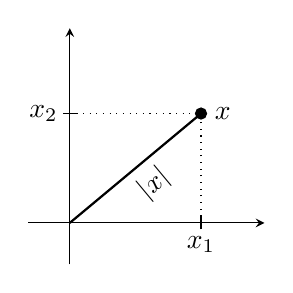
\begin{tikzpicture}% coordinates
            \begin{axis}[
                axis equal,
                axis lines=middle,
                no marks,
                xmin=-1,
                xmax=8,
                ymin=-1,
                ymax=8,
                enlargelimits, 
                scale only axis, 
                height=3cm, 
                width=3cm,
                xtick={0},
                ytick={0}
            ]
            \node [fill=white,anchor=center] at (6, -1) {$x_1$};
            \addplot [no marks, black ]coordinates {
				(6,-0.3)
                (6, 0.3)
			};
            \node [fill=white,anchor=center] at (-1.2, 5) {$x_2$};
            \addplot [no marks, black ]coordinates {
				(-0.3, 5)
                (0.3, 5)
			};
            \addplot [only marks, black ]coordinates {
				(6, 5)
			};
            \node [fill=white,anchor=center] at (7, 5) {$x$};
            \addplot [no marks, black, dotted ]coordinates {
				(6, 0)
                (6, 5)
			};
            \addplot [no marks, black, dotted ]coordinates {
				(0, 5)
                (6, 5)
			};
            \node [fill=white,anchor=center, rotate around={39.80:(0,0)}] at (3, 2.2) {$|x|$};
            \addplot [no marks, black, thick]coordinates {
				(0, 0)
                (6, 5)
			};
            
            \end{axis}
        \end{tikzpicture}
    \end{center}
    
Invece, per $ a \in \R $, \[
    |a|=\sqrt{a^{2}}=\begin{cases}
        a &a\ge 0\\
        -a & a<0
    \end{cases}
\] ovvero diventa equivalente al \textit{valore assoluto} di $ a $.
\begin{center}
    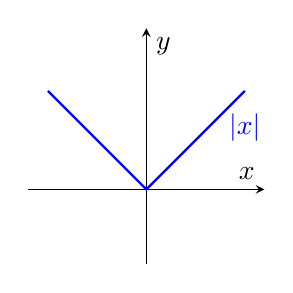
\begin{tikzpicture}% coordinates
        \begin{axis}[
            xlabel=$x$, 
            ylabel=$y$,
            axis equal,
            axis lines=middle,
            no marks,
            xmin=-8,
            xmax=8,
            ymin=-1,
            ymax=8,
            enlargelimits, 
            scale only axis, 
            height=3cm, 
            width=3cm,
            xtick={0},
            ytick={0}
        ]
        \node [fill=white,anchor=center] at (8, 5) {\textcolor{blue}{$|x|$}};
        \addplot [no marks, blue, thick] coordinates {
            (-8, 8)
            (0, 0)
            (8, 8)
        };
        \end{axis}
    \end{tikzpicture}
\end{center}
}

\proprieta[del modulo]{
    $ \forall\, x,y \in \R^{n} $, $ \forall\, \lambda, \mu \in \R $ si ha

    $ \eta \hspace{0.2em} $$\left\{ %\{
	  \begin{minipage}{0.8\textwidth}
	    \begin{enumerate}
            \item $|x|\ge 0; \quad |x|=0 \,\iff\, x=0    $    
            \item $|\lambda x| = |\lambda|\,|x|$
            \item $|x+y| \le |x|+ |y|$ (disuguaglianza triangolare)
        \end{enumerate}
	  \end{minipage}\right.$

    
}

\osservazione{
    \begin{align}
        |x|=|(x-y)+y|\le |x-y|+|y|\, &\iff\, |x|-|y|\le |x-y|\label{aaaaa}\\
        |y|=|(y-x)+x|\le |x-y|+|x| \,&\iff\, |x|-|y|\ge -|x-y|\label{bbbbb}
    \end{align}
    Mettendo insieme \eqref{aaaaa} e \eqref{bbbbb} otteniamo \[
        \forall\, x,y \in \R^{n}\quad -|x-y|\le |x|-|y|\le |x-y|
    \] da cui \begin{equation}
        \big| |x|-|y|\big| \le |x-y|
    \end{equation}
}

\nota{Ricordare che, dato $ a\ge 0 $, $ x \in \R $, \[
    |x|\le a \quad \iff\quad -a\le x\le a
\]}

\definizione{}{
    Dati $ x, y \in \R^{n} $ diciamo \textit{distanza} di $ x $ da $ y $\begin{equation}
        d(x,y):= |x-y|=\sqrt{\sum_{j=1}^{n}(x_{j}-y_{j})^{2} }
    \end{equation}
}

\proprieta[della distanza]{
    $ \forall\, x,y, z \in \R^{n} $ si ha 

    $ \mathcal{D} \hspace{0.2em} $$\left\{ %\{
	  \begin{minipage}{0.8\textwidth}
	    \begin{enumerate}
            \item $d(x,y)\ge 0;\quad d(x,y)=0\,\iff\, x=y$;
            \item $ d(x,y)=d(y,x)  $;
            \item $ d(x,y)\le d(x,z)+d(y,z)$ (disuguaglianza triangolare).
        \end{enumerate}
	  \end{minipage}\right.$
}

\definizione{}{
    $ \R^{n} $ e ogni altro insieme dotato di somma ($+$), prodotto per uno scalare e norma (distanza), sono detti \textit{spazi vettoriali normati} o \textit{spazi vettoriali metrici}.
}

\section{Punti di accumulazione}

\definizione{}{
    Sia $ x_0 \in \R^{n} $, $ r>0 $, diciamo \textit{intorno (sferico)} di $ x $ di raggio $ r $
    \begin{equation}
        B_{r}(x)=\{z \in \R^{n};\, d(z,x)<r\}=\{z \in \R^{n};\, |z-x|<r\}
    \end{equation}
}

\esempio{}{
    In $ \R^{2} $, dato $ x=(x_1, x_2) $ \begin{multline*}
        B_{r}(x)=\{z=(z_1, z_2) \in \R^{2}; |z-x|<r\}=\\
        =\{z=(z_1, z_2) \in \R^{2}; (z_1-x_1)^{2}+(z_2-x_2)^{2}<r^{2}\}
    \end{multline*} 
    
    $\implies$ $ B_{r}(x) $ è un cerchio di centro $ x  $ e raggio $ r $, escluso il bordo.
}

Si indica anche con $ B(r, x) $, $ B(x,r) $, oppure $ B(x) $ se non è importante il valore del raggio.

In generale diciamo che $ I(x) $ è \textit{intorno} di $ x $ se \[
    \exists\, r>0\,\tc\, B_{r}(x) \subseteq I(x) 
\]

\definizione{}{
    Dato $ E \subseteq \R^{n} $, diciamo che $ E $ è \textit{limitato} se \[
        \exists\,R>0 \,\tc\, E \subseteq B_{R}(\underline{0}) 
    \]
}

\definizione{}{
    Sia $ E \subseteq \R^{n} $, $ x_0 \in \R^{n} $. Diciamo che $ x_0 $ è un \textit{punto di accumulazione} per $ E $ se \begin{equation}
        \forall\,r >0\, \exists\, x \in R, x \neq x_0\,\tc\, x \in B_{r}(x_0) 
    \end{equation}

    Se $ x $ di accumulazione per $ E $ $\nLeftrightarrow $ $ x \in E $
}

\esempio{}{
    Dato $ E=F\cup\{p\} $
    \begin{center}
    \begin{tikzpicture}[scale=2.5]
        \draw plot [smooth, tension=0.6] coordinates {(4.4,0.4) (5,0.2) (5.8,0.6) (6.5773,0.5421) (6.4905,1.1074)};  
        \draw [dashed] plot [smooth, tension=0.6] coordinates {(6.4905,1.1074) (5.9752,1.2828) (5.4,1.4) (4.6,1) (4.4,0.4)};
        \node at (7, 1.5) {$p$};
        \node at (5.5, 0.9) {$F$};
        \fill (6.9, 1.5) circle (0.023cm);
        \fill [green] (5,0.2) circle (0.023cm);
        \node at (5, 0.1) {\textcolor{green}{$x_0$}};
        \fill [green] (5.4,1.4) circle (0.023cm);
        \node at (5.4, 1.5) {\textcolor{green}{$x_1$}};
    \end{tikzpicture}
\end{center}
\begin{itemize}
    \item $ x_0 $ è di accumulazione;
    \item $ x_1 $ è di accumulazione;
    \item $ p $ non è di accumulazione.
\end{itemize}
}

\definizione{}{
    Se $ x_0 \in E $, $ x_0 $ non è di accumulazione, allora $ x_0 $ è un \textit{punto isolato} di $ E $.
}

\esempio{}{
    \[
        E=\big\{x=1+1/n, n \in \N\setminus \{0\}\big\}
    \]   
    $ \forall\, n $, $ x_{n}  $ non è punto di accumulazione. Se $ y \in E $ 
    
    $\implies$ $ y $ non è di accumulazione.
    
    $ a=1 $ è l'unico punto di accumulazione per $ E $, e $ 1 \notin E $. \[
        |1-x_{n}|=|1-(1+1/n)|=1/m
    \] quindi \[
        \forall\, \varepsilon>0\, \exists\, n \,\tc\, x_{n} \in B_{ \varepsilon}(1) 
    \] scegliendo $ n $ tale che $ 1/n< \varepsilon $ 
    
    $\implies$ $ n>1/ \varepsilon $
}

\esempio{}{
    $ n \in \N $ non è punto di accumulazione, $ \N $ non ammette alcun punto di accumulazione (vale anche per $ \Z $). Inoltre, un qualsiasi sottoinsieme di $ \R $, \textit{finito}, non ammette punti di accumulazione.
}

\definizione{}{Se $ E \subseteq \R^{n} $ non ammette alcun punto di accumulazione, si dice che $ E $ è \textit{discreto}

$ \N $, $ \Z $ e gli insiemi finiti sono discreti. $ \Q $ non è discreto;

numerabile $ \nRightarrow $ discreto, ma discreto $ \implies $ finito e numerabile.
}

\notazione{}{
    Dato $ E \in \R^{n} $, $ E' $ è l'insieme dei punti accumulazione di $ E $, e prende il nome di \textit{insieme derivato}.

    $ E'\neq \emptyset $ $ \iff $ $ E $ è discreto.
}

\proprieta{}{
    $ x_0 $ è di accumulazione per $ E $ 
    
    $ \iff $ $ \forall\, r > 0 $, $ B_{r}(x_0)  $ contiene infiniti punti.
    \begin{proof}
        $ \exists\, r>0 $ tale che $ \exists\, x_1\neq x_0 $, $ x_1 \in B_{r}(x_0)  $

        $ \exists\, r_1 >0 $ tale che $ x_1 \notin B_{r_{1} }(x_0)  $, $ \exists\, x_2 \in B_{r_{1} }(x_0)  $

        $ \exists\, r_2 >0 $ tale che $ x_1, x_2 \notin B_{r_{2} }(x_0)  $, $ \exists\, x_3 \in B_{r_{2} }(x_0)  $

        \dots

        Procedendo in questo modo ottengo una sequenza di punti \[
            x_1, x_2, \cdots, x_{n}, \cdots \quad \forall\, n , \, x_{n} \in B_{r}(x_0)\qedhere   
        \]
    \end{proof}
}
\proprieta{}{
    Dati due insieme $ A, B \subseteq \R $, assumiamo che $ \forall\, a \in A, b \in B $, $ a\le b $ 
    
    $\implies$ $ \sup A \le \inf B $
}

\teorema[(di Bolzano-Weierstrass)]{bolzweierstrrdsdkkslkjf}{
    Sia $ E \subseteq \R^{n} $, $ E $ limitato e $ E $ infinito. 
    
    $\implies$ $ E $ ammette almeno un punto di accumulazione $ x_0 $
}
\osservazione{
    $ E $ limitato $ \implies $ $ \exists\,r>0 $ tale che $ E \subseteq B_{r}(0)  $

    $ E $ infinito $ \iff $ $ E $ contiene infiniti punti
}
\dimostrazione{bolzweierstrrdsdkkslkjf}{
    Per semplicità dimostriamo il teorema in $ \R^{2} $\begin{itemize}
        \item [1$^{o}$ passo] Individuiamo $ x_0 $ candidato punto di accumulazione (\textit{i});
        \item [2$^{o}$ passo] dimostriamo che $ x_0 $ è davvero punto di accumulazione (\textit{ii}).
    \end{itemize} 
    \rule{7em}{.4pt}
    \begin{itemize}
        \item [(\textit{i})] Sappiamo che $ E $ è limitato 
        
        $\implies$ $ \exists\, T_{0}=[p_0, q_0]\times [r_0, s_0]  $ tale che $ E \subseteq T_{0}  $
        \begin{center}
            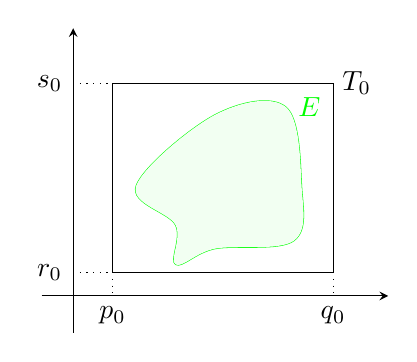
\begin{tikzpicture}
                \draw [green] plot [smooth cycle, tension=0.6] coordinates {(1, 2) (1.5, 1.5) (1.5, 1) (2, 1.2) (3, 1.3) (3.1, 2) (2.9, 3) (2, 2.9)};
                \fill [green!5] plot [smooth cycle, tension=0.6] coordinates {(1, 2) (1.5, 1.5) (1.5, 1) (2, 1.2) (3, 1.3) (3.1, 2) (2.9, 3) (2, 2.9)};
                \node at (3.2, 3) {\textcolor{green}{$E$}};  
                \draw (0.7, 0.9) -- (3.5, 0.9) -- (3.5, 3.3) -- (0.7, 3.3) -- cycle;
                \node at (3.8, 3.3) {$T_0$}; 
                \draw [-stealth] (0.2, 0.13) -- (0.2, 4); 
                \draw [-stealth] (-0.2, 0.6) -- (4.2, 0.6); 
                \draw [dotted] (0.7, 0.9) -- (0.7, 0.6);
                \draw [dotted] (3.5, 0.9) -- (3.5, 0.6);
                \draw [dotted] (0.2, 0.9) -- (0.7, 0.9);
                \draw [dotted] (0.2, 3.3) -- (0.7, 3.3);
                \node at (0.7, 0.35) {$p_0$};
                \node at (3.5, 0.35) {$q_0$};
                \node at (-0.1, 0.9) {$r_0$};
                \node at (-0.1, 3.3) {$s_0$}; 
            \end{tikzpicture}
        \end{center}

        Dividiamo $ T_{0} $ in quattro rettangoli: \[
            T_0^{1}, T_0^{2}, T_0^{3}, T_0^{4}
        \] 
        
        $\implies$ almeno uno contiene infiniti punti di $ E $. Assumiamo che sia $ T_0^{2} $

        \begin{center}
            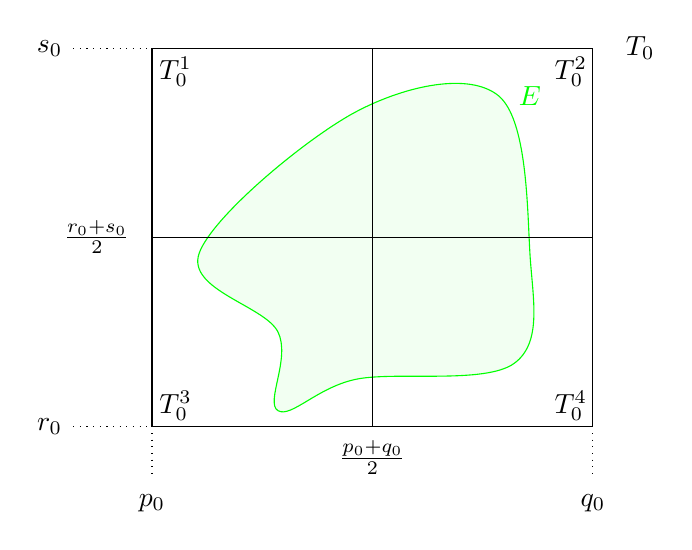
\begin{tikzpicture}[scale=2]
                \fill [green!5] plot [smooth cycle, tension=0.6] coordinates {(1, 2) (1.5, 1.5) (1.5, 1) (2, 1.2) (3, 1.3) (3.1, 2) (2.9, 3) (2, 2.9)};
                \draw [green] plot [smooth cycle, tension=0.6] coordinates {(1, 2) (1.5, 1.5) (1.5, 1) (2, 1.2) (3, 1.3) (3.1, 2) (2.9, 3) (2, 2.9)};
                \node at (3.1, 3) {\textcolor{green}{$E$}};  
                \draw (0.7, 0.9) -- (3.5, 0.9) -- (3.5, 3.3) -- (0.7, 3.3) -- cycle;
                \draw (2.1, 0.9) -- (2.1, 3.3);
                \node at (2.1, 0.7) {$\frac{p_0+q_0}{2}$};
                \node at (0.35, 2.1) {$\frac{r_0+s_0}{2}$};
                \draw (0.7, 2.1) -- (3.5, 2.1);
                \node at (3.8, 3.3) {$T_0$}; 
                \draw [dotted] (0.7, 0.9) -- (0.7, 0.6);
                \draw [dotted] (3.5, 0.9) -- (3.5, 0.6);
                \draw [dotted] (0.2, 0.9) -- (0.7, 0.9);
                \draw [dotted] (0.2, 3.3) -- (0.7, 3.3);
                \node at (0.7, 0.41) {$p_0$};
                \node at (3.5, 0.41) {$q_0$};
                \node at (0.05, 0.9) {$r_0$};
                \node at (0.05, 3.3) {$s_0$};
                \node at (0.85, 3.15) {$T_0^{1}$};
                \node at (3.36, 3.15) {$T_0^{2}$};
                \node at (0.85, 1.03) {$T_0^{3}$};
                \node at (3.36, 1.03) {$T_0^{4}$}; 
            \end{tikzpicture}
        \end{center}

        Poniamo $ T_1=T_0^{2} $, $ T_1=[p_1, q_1]\times [r_1, s_1] $\begin{align*}
            p_1& =\frac{p_0+q_0}{2}\quad &q_1=q_0\\
            r_1&=\frac{r_0+s_0}{2}\quad &s_1=s_0
        \end{align*}

        Dividiamo $ T_1 $ in quattro rettangoli. Almeno uno contiene infiniti punti di $ E $. Ne scegliamo uno: $ T_1^{3} $.

        \begin{center}
            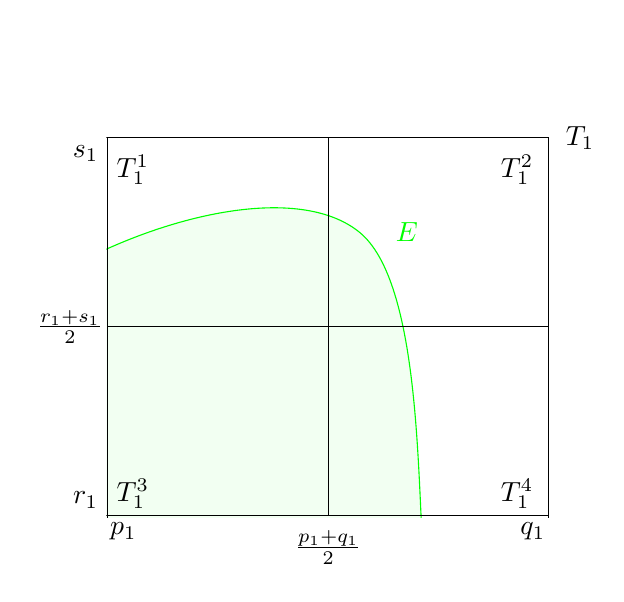
\begin{tikzpicture}[scale=4]
                \node at (2.8, 2.0) {$\frac{p_1+q_1}{2}$};
                \node at (1.98, 2.7) {$\frac{r_1+s_1}{2}$};
                \node at (2.15, 2.05) {$p_1$};
                \node at (3.45, 2.05) {$q_1$};
                \node at (2.03, 2.15) {$r_1$};
                \node at (2.03, 3.25) {$s_1$};
                \clip (2.096,2.096) rectangle (3.65,3.65);
                \fill [green!5] plot [smooth cycle, tension=0.6] coordinates {(1, 2) (1.5, 1.5) (1.5, 1) (2, 1.2) (3, 1.3) (3.1, 2) (2.9, 3) (2, 2.9)};
                \draw [green] plot [smooth cycle, tension=0.6] coordinates {(1, 2) (1.5, 1.5) (1.5, 1) (2, 1.2) (3, 1.3) (3.1, 2) (2.9, 3) (2, 2.9)};
                \node at (3.05, 3) {\textcolor{green}{$E$}};  
                \draw (0.7, 0.9) -- (3.5, 0.9) -- (3.5, 3.3) -- (0.7, 3.3) -- cycle;
                \draw (2.1, 0.9) -- (2.1, 3.3);
                \node at (2.1, 0.7) {$\frac{p_0+q_0}{2}$};
                \node at (0.35, 2.1) {$\frac{r_0+s_0}{2}$};
                \draw (0.7, 2.1) -- (3.5, 2.1);
                \node at (3.6, 3.3) {$T_1$}; 
                \draw [dotted] (0.7, 0.9) -- (0.7, 0.6);
                \draw [dotted] (3.5, 0.9) -- (3.5, 0.6);
                \draw [dotted] (0.2, 0.9) -- (0.7, 0.9);
                \draw [dotted] (0.2, 3.3) -- (0.7, 3.3);
                \node at (0.7, 0.41) {$p_0$};
                \node at (3.5, 0.41) {$q_0$};
                \node at (0.05, 0.9) {$r_0$};
                \node at (0.05, 3.3) {$s_0$};
                \node at (2.18, 3.2) {$T_1^{1}$};
                \node at (3.4, 3.2) {$T_1^{2}$};
                \node at (2.18, 2.17) {$T_1^{3}$};
                \node at (3.4, 2.17) {$T_1^{4}$};
                \draw (2.8, 2.1) -- (2.8, 3.3);
                \draw (2.1, 2.7) -- (3.5, 2.7);
            \end{tikzpicture}
        \end{center}

        Poniamo $ T_2=T_1^{3} $, $ T_2=[p_2, q_2]\times [r_2, s_2] $\begin{align*}
            p_2&=p_1\quad & q_2=\frac{p_1+q_1}{2}\\
            r_2&=r_1\quad & s_2=\frac{r_1+s_1}{2}
        \end{align*}

        Procediamo in questo modo, passo dopo passo: otteniamo una sequenza di rettangoli tutti contenenti infiniti punti di $ E $: \begin{align*}
            T_0&=[p_0, q_0]\times [r_0, s_0]\\
            T_1 \subseteq T_0 & = [p_1, q_1]\times [r_1, s_1] \\ &\implies\, s_1-r_1=\frac{s_0-r_0}{2}, \:q_1-p_1=\frac{q_0-p_0}{2}\\
            &\cdots\\
            T_{n} \subseteq T_{n-1} \subseteq \cdots \subseteq T_0 &= [p_{n} , q_{n}]\times [r_{n}, s_{n}]\\
            &\implies\, s_{n}-r_{n}=\frac{s_0-r_0}{2^{n}},\: q_{n}-p_{n}=\frac{q_0-p_0}{2^{n}}    
        \end{align*}

        Consideriamo l'insieme degli estremi destri e sinistri delle basi: \[
            P=\{p_0, p_1, \cdots, p_{n}, \cdots \},\qquad Q=\{q_0, q_1, \cdots, q_{n}, \cdots \}
        \]

        Per costruzione, $ P $ e $ Q $ sono limitati, dunque ammettono estremo superiore e inferiore. Inoltre $ \forall\, p \in P $, $ \forall\, q \in Q $, $ p<q $. Allora per la proprietà vista precdentemente, $ \sup P \le \inf Q $. Inoltre, \[
            \forall\,n,\: p_{n}\le \sup P,\: q_{n}\ge \inf Q
        \]
        quindi \[
            0\le \inf Q - \sup P \le q_{n}-p_{n}\le \frac{q_0-p_0}{2^{n}}  
        \]

        Allora $ \forall\, \varepsilon>0 $, $ 0\le \inf Q- \sup P\le \varepsilon $: è sufficiente che \[
            \frac{q_0-p_0}{2^{n}}< \varepsilon
        \] 
        
        $\implies$ $ \inf Q =\sup P $ % TODO perché posso affermare questo? non serve il teorema del confronto? posso applicarlo senza problemi? 
        \[
            x_1=\sup P = \inf Q
        \]

        Ripetiamo lo stesso ragionamento sulle altezze $ [r_{j}, s_{j}  ] $: \begin{align*}
            R&=\{r_0, r_1, \cdots, r_{n}, \cdots \}\\
            S&=\{s_0, s_1, \cdots, s_{n}, \cdots \}
        \end{align*}
        Allora $ \inf S =\sup R =x_2 $.

        Quindi $ x_0=(x_1, x_2) $ è il candidato punto di accumulazione.
        \item [(\textit{ii})] Dimostriamo che $ x_0 $ è di accumulazione:
        
        $ \forall\,n $ $ x_0 \in T_{n} $, % TODO posso dirlo senza dimostrarlo?
        ma $ T_{n} $ contiene infiniti punti di $ E $. Inoltre, $ T_{n} \subseteq T_0 $.

        $ \forall\, \varepsilon>0 $, $ \exists\, T_{c} \subseteq B_{ \varepsilon} (x_0)  $ 
        
        $\implies$ $ \forall\, \varepsilon $, $ B_{ \varepsilon}  $ contiene infiniti punti di $ E $. 
        
        $\implies$ $ x_0 $ è di accumulazione per $ E $.\qed
    \end{itemize}
}
\section{Topologia} 
\definizione{}{
    Sia\marginnote{4 ott 2021} $ A \subseteq \R^{n} $, $ A $ si dice \textit{aperto} in $ \R^{n} $ se $ \forall\, x \in A $ $ \exists\, r>0 $ tale che $ B_r(x) \subseteq A $
}

\esempio{\label{es:gigio}\newcounter{estizio}\addtocounter{estizio}{\theesempi}
    $ R>0 $, sia \[D_{R}=\{x \in \R^{n}\,\tc\: |x| < R\} \] il disco di raggio $ R $. Dimostriamo che $ D_{R} $ è aperto.

    Dato $ x \in D_{R}  $, consideriamo $ r>0 $ tale che $ 0<r<R-|x| $ 
    
    $\implies$ $ r+|x|<R $.

    Verifichiamo che $ B_{r} \subseteq D_{R}$ ossia che $ \forall\, y \in B_{r}(x) $, $ |y|<R $ \[
        |y|=|y+x-x|\le \parentesi{<r}{|y-x|}+|x| \le r - |x| <R
       \] 
       
       $\implies$ $ B_{r}(x) \subseteq D_{R}$ 
       
       $\implies$ $ D_{R}  $ è aperto.

       $ D_{R}  $ si chiamerà \textit{disco aperto} di $ R $, ed è aperto e non limitato.
       \begin{center}
        In $ \R^{2} $

           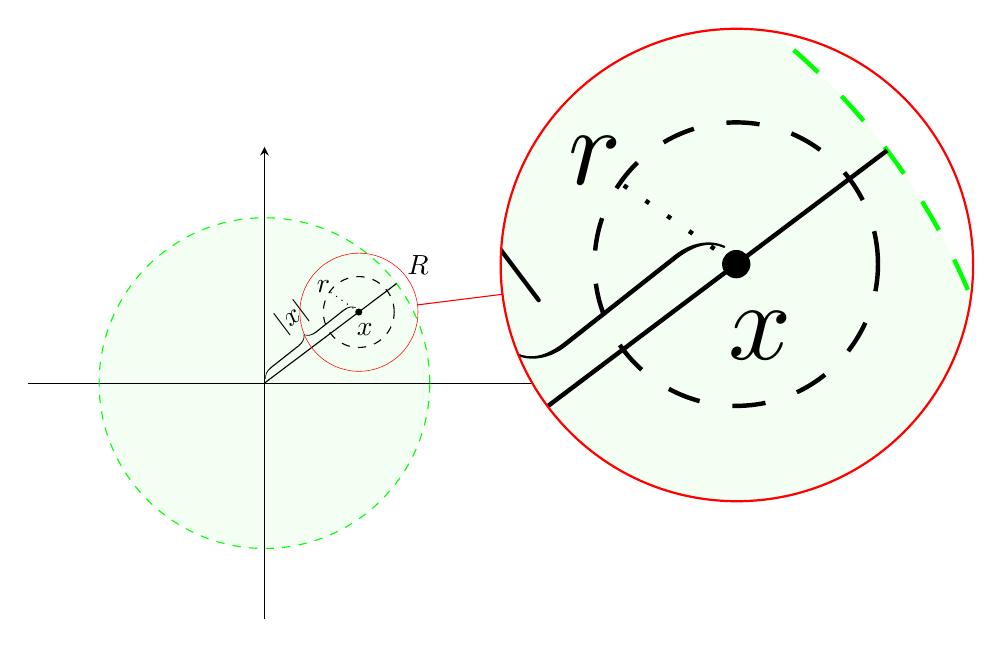
\begin{tikzpicture}[scale=1.5, spy using outlines={circle, magnification=4, size=6cm, connect spies}]
            \fill [green!5] (0,0) circle (1.4);
               \draw [-stealth] (-2, 0) -- (3, 0);
               \draw [-stealth] (0, -2) -- (0, 2);
               \draw [dashed, green] (0,0) circle (1.4);
               \draw (1.11808971407,0.84254103241) -- (0,0);
               \fill (0.79863551004,0.60181502315) circle (0.03);
               \draw [dashed] (0.79863551004,0.60181502315) circle (0.3);
               \draw [dotted] (0.79863551004,0.60181502315) -- (0.55288989675, 0.77388795405);
               \node at (0.85, 0.45) {$x$};
               \draw [decorate, decoration = {calligraphic brace, raise = 2pt, amplitude = 4pt}] (0.04,0) -- (0.80263551004,0.60181502315);
                \node [rotate=37] at (0.235, 0.555) {$|x|$};
                \node at (1.3, 1) {$R$};
                \node at (0.5, 0.82) {$r$};
                \begin{scope}
                    \spy[red,size=6cm] on (1.2,0.9) in node [fill=white] at (4,1);
                \end{scope}
           \end{tikzpicture}
       \end{center}
}
\begin{minipage}{\textwidth}
\esempio{}{
    Sia $ E=\{z=(x,y) \in \R^{n}\,\tc\, y<x\} $
    \begin{center}
        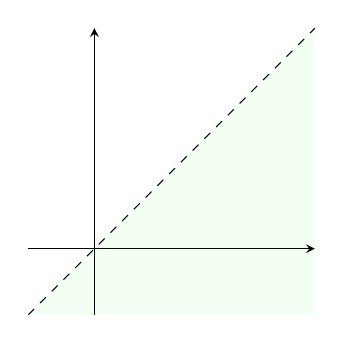
\begin{tikzpicture}[scale=1.4]
            \draw [color=black!0, fill=green!5] (-0.6, -0.6) -- (2, -0.6) -- (2,2) -- cycle;
            \draw [-stealth] (-0.6, 0) -- (2, 0);
            \draw [-stealth] (0,-0.6) -- (0,2);
            \draw [dashed] (-0.6, -0.6) -- (2,2);
        \end{tikzpicture}
    \end{center}

    $ z_0 \in E $, $ z_0=(x_0, y_0) $, $ y_0<x_0 $. Consideriamo la distanza di $ z_0 $ dalla retta $ s:y=x $, $ d(z_0, s) $ \[
        d(z_0, s) =\frac{|x_0-y_0|}{\sqrt{2}}
    \]
    
    Fissato $ 0<r<\frac{|x_0-y_0|}{\sqrt{2}}\displaystyle $ 
    
    $\implies$ $ B_{r}(z_0) \subseteq E  $. $ E $ è aperto e non limitato.
}
\end{minipage}
\esempio{}{
    Sia $ R>0 $, \[
        G_{R}=\{x \in \R^{n}; |x|\ge R\} 
    \] (vedasi Figura \ref{fig:1})
    \begin{figure}
    \begin{center}
        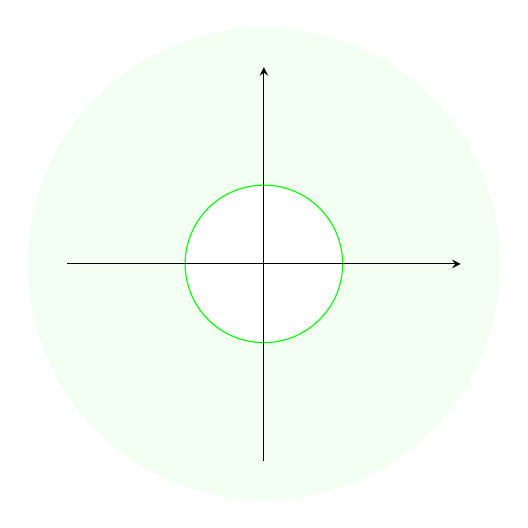
\begin{tikzpicture}
            \fill [green!5] (0,0) circle (3);
            \fill [white] (0,0) circle (1);
            \draw [green] (0,0) circle (1);
            \draw [-stealth] (-2.5, 0) -- (2.5, 0);
            \draw [-stealth] (0, -2.5) -- (0, 2.5);
        \end{tikzpicture}
    \end{center}
    \caption{$ G_{R}  $ in $ \R^{2} $}
    \label{fig:1}
    \end{figure}
    \begin{gather*}
        x_0=(R, 0, \cdots, 0)\\
        x_0 \in G_{R} \\
        \forall\, \varepsilon>0\quad \begin{aligned}
            x_1&=(R+ \varepsilon, 0, \cdots, 0) \subseteq G_{R}\\
            x_2&=(R- \varepsilon, 0, \cdots, 0) \nsubseteq  G_{R}
        \end{aligned}
    \end{gather*} 
    
    $\implies$ $ G_{R}  $ non è aperto.
}
\definizione{}{
    $ A \subseteq \R^{n} $ è \textit{chiuso} (in $ \R^{n} $) se l'insieme $ A^{C} $ è aperto: \[A^{C}= \R^{n}\setminus A = \{x \in \R^{n}; x \notin A\}.
    \]
}
\esempio{}{
    Dato $G_{R}=\{x \in \R^{n}; |x|\ge R\} $, \[D_{R}=G_{R}^{C}=\{x \in \R^{n}, |x|<R \} \] è aperto (vedasi esempio \hyperref[es:gigio]{\thesection.\theestizio}) 
    
    $\implies$ $ G_{R}  $ è chiuso.
}
\esempio{}{
    Sia \begin{align*}
        \overline{D_{R}}&=\{x \in \R^{n}, \, |x|\le R\}\\
        \overline{D_{R}^{C}}=\R^{n}\setminus \overline{D_{R}}& =\{x \in \R^{n},\,|x|>R\}
    \end{align*}

    Sia $ 0<r<|x|-R $. Consideriamo $ z \in B_{r}(x)  $
    \begin{equation*}
        |z|=|z-x+x|=|x-(x-z)|
        \ge \big||x|-\parentesi{<r}{|x-z|}\big|\ge |x|-r>R
    \end{equation*} 

    $\implies$ $ \forall\, z \in B_{r}(x)$, $ |z|>R $ 
    
    $\implies$ $ B_{r}(x) \subseteq \overline{D_{R}^{C} }  $ 
    
    $\implies$ $ \overline{D_{R}^{C} } $ è aperta 
    
    $\implies$ $ \overline{D_{R} } $ è chiuso.
}
\esempio{}{
    Dati $ 0<r<R $, è definita corona circolare l'insieme:
    \[
        C_{R,r}=\big\{z=(x,y) \in \R^{2}; r^{2}<x^{2}+y^{2}\le R^{2}\big\} 
    \]
    \begin{center}
        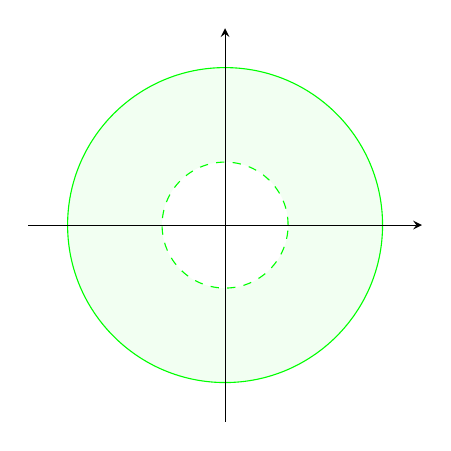
\begin{tikzpicture}
            \fill [green!5] (0,0) circle (2);
            \fill [white] (0,0) circle (0.8);
            \draw [green] (0,0) circle (2);
            \draw [dashed, green] (0,0) circle (0.8);
            \draw [-stealth] (-2.5, 0) -- (2.5, 0);
            \draw [-stealth] (0, -2.5) -- (0, 2.5);
        \end{tikzpicture}
    \end{center}
    $ C_{R, r}  $ non è aperto, \[
        C_{R,r}^{C}=\big\{z=(x,y) \in \R^{2}, x^{2}+y^{2}\le r^{2}\,\lor\, x^{2}+y^{2}> R^{2}\big\} 
    \] 
    
    $\implies$ $ C_{R,r}^{C} $ non è aperto.

    Concludiamo che $ C_{R,r}  $ non è né aperto né chiuso.
}  
\paragraph{Domanda}\begin{itemize}
    \item $ \emptyset $ è aperto? \[
        x \in \emptyset \,\implies\, \exists\, r>0\,\tc\, B_{r}(x) \subseteq \emptyset 
    \] 
    
    $\implies$ è sempre vera perché $ x \in \emptyset $ è falsa. 
    
    $\implies$ $ \emptyset $ è aperto.
    \item $ \R^{n} $ è aperto? $ \forall\,x \in \R^{n} $, $ \exists\, r>0 $ tale che $ B_{r}(x) \subseteq \R^{n}  $.
    \item $ \R^{n}=\R^{n}\setminus \emptyset $ 
    
    $\implies$ $ \R^{n} $ è complementare di un insieme aperto, ovvero è chiuso.
    \item $ \emptyset = \R^{n}\setminus \R^{n} $ 
    
    $\implies$ $ \emptyset $ è complementare di un insieme aperto, ovvero è chiuso.
    \item $ \emptyset $ e $ \R^{n} $ sono sia aperti che chiusi: sono gli unici due.
\end{itemize}
\definizione{}{
    Sia $ E \subseteq \R^{n} $ \begin{itemize}
        \item $ x_0 \in E $, diciamo che $ x_0 $ è \textit{interno} ad $ E $ se $ \exists\, r>0 $ tale che $ B_{r}(x_0) \subseteq E $;
        \item $ x_1 \in \R^{n} $, diciamo che $ x_1 $ è \textit{esterno} ad $ E $ se $ x_1 $ è interno a $ E^{C}=\R^{n}\setminus E $ 
        
        $\implies$ $ \exists\, r_1>0 $ tale che $ B_{r_1}(x_1) \subseteq E^{C}  $
        \item $ x_2 \in \R^{n} $, diciamo che $ x_2 $ è \textit{di frontiera} per $ E $ se $ x_2 $ non è interno ad $ E $ e $ x_2 $ non è esterno ad $ E $.
    \end{itemize}
} 
\notazione{}{
    $\mathring{E}$ è l'insieme di tutti i punti interni di $ E $: \begin{itemize}
        \item $ x_0 $ interno $\implies$ $ x_0 \in \mathring{E}$;
        \item $ x_0 $ esterno $\implies$ $ x_0 \in \mathring{E}^{C}$;
        \item $ x_0 $ di frontiera $\implies$ $ x_0 \notin\mathring{E} \,\land\, x_0\notin\mathring{E}^{C}$ 
        
        $\implies$ $ x_0 \in \partial E $
    \end{itemize}
}
\osservazione{}{
    \begin{itemize}
        \item $ \partial E =\partial E^{C} $;
        \item $ x_0 \in \mathring{E}$ $\implies$ $ x_0 \in E $ $\implies$ $ \mathring{E} \subseteq E $;
        \item $ x_0 \in \partial E $ non abbiamo informazioni sull'appartenenza di $ x_0 $ ad $ E $.
    \end{itemize}
}
\proprieta[(di caratterizzazione degli aperti)]{
    Dato $ A \subseteq \R^{n} $, 
    
    $ A $ è aperto $ \iff $ $ A=\mathring{A} $.
}
\begin{proof} Dimostriamo le due implicazioni:

    \begin{itemize}
        \item [``$\impliedby$''] $ \forall\,x \in A $ $\implies$ $ x \in \mathring{A}$ 
        
        $\implies$ $ \exists\, r>0$ tale che $ B_{r}(x) \subseteq A$ 
        
        $\implies$ $ A $ è aperto.
        \item [``$\implies$''] Assumiamo $ A $ aperto; $ \mathring{A} \subseteq A $ sempre.
        
        $ \forall\, x \in A $, $ \exists r >0 $ tale che $ B_{r}(x) \subseteq A$ 
        
        $\implies$ $x$ è interno 
        
        $\implies$ $ A \subseteq \mathring{A} $\qedhere
    \end{itemize}
\end{proof}

\teorema[(di caratterizzazione dei chiusi)]{carchiusdijooijooijdjkdjjdjdjdj}{
    Dato $ E \subseteq \R^{n} $, le seguenti proprietà sono equivalenti
    \begin{itemize}
        \item [(\textit{i})] $ E $ è chiuso;
        \item [(\textit{ii})] $ \partial E \subseteq E$;
        \item [(\textit{iii})] $ E' \subseteq E $, dove con $ E' $ indichiamo tutti i punti di accumulazione di $ E $.
    \end{itemize}
}
\dimostrazione{carchiusdijooijooijdjkdjjdjdjdj}{
    \begin{itemize}
        \item [(\textit{i}) $ \implies $ (\textit{ii})] $ E $ chiuso $ \implies $ $ \partial E \subseteq E $
        
        $ \forall\,x \in \partial E $, $ x\notin \mathring{E}^{C} $, ma $ \mathring{E}^{C} $ è aperto 
        
        $\implies$ $ \mathring{E}=\mathring{E}^{C} $ 
        
        $\implies$ $ x \in E $ 
        
        $\implies$ $ \partial E \subseteq E $
        \item [(\textit{ii}) $ \implies $ (\textit{iii})] $ \partial E \subseteq E$ $ \implies $ $ E' \subseteq E $
        
        \[
            \forall\, x \in E', \forall\, r >0\: \exists\, y \neq x \in E, y \in B_{r}(x) 
        \]
        osserviamo che $ x \in E' $ $\implies$ $ x \notin \mathring{E^{{C}}} $, infatti se per assurdo $ x \in \mathring{E^{{C}}} $ \[
            \exists\, r>0\,\tc\: B_{r}(x) \subseteq E^{C} \,\implies\, B_{r}(x)\cap E = \emptyset  
        \] 
        
        $\implies$ $ x \notin E' $
        \begin{itemize}
            \item caso \textit{a}: $ x \in \partial E $, visto che $ \partial E \subseteq E $ 
            
            $\implies$ se $ x \in E' $, allora $ x \in E $
            \item caso \textit{b}: $ x \in \mathring{E} $ $ \implies $ $ x \in E $
            
            Se $ x \in E' $, allora $ x \in E $
        \end{itemize}
        Ne risulta che $ E' \subseteq E $
        \item [(\textit{iii}) $ \implies $ (\textit{i})]
        %%%%%%%%%
    \end{itemize}
}
\part{Funzioni e Successioni}
\section{Corrispondenze}
Siano\marginnote{5 ott 2021} $ X, Y $ insiemi, e consideriamo $ P(x,y) $ predicato su $ x \in X $ e su $ y \in Y $.
\esempi{}{
    \begin{itemize}
        \item $X$: fantini di una squadra\\ $Y$: cavalli della stessa squadra\\ $ P(x,y) $: $ x $ ha cavalcato almeno una volta $ y $;
        \item $ X=Y= \R $; $ P(x,y) $: $ x^{2}+y^{2}=1 $;
        \item $ X=Y= \R $; $ P(x,y) $: $ y=x^{2} $.
    \end{itemize}
}

\definizione{}{Una \textit{corrispondenza} $ \mathfrak{F} $ tra gli elementi di $ X $ e di $ Y $ è un predicato binario $ P(x,y) $ nelle variabili $ x \in X $, $ y \in Y $.

Diciamo che $ x \in X $ è in corrispondenza con $ y \in Y $ se $ P(x,y) $ è verificata. Scriviamo \[
    y=\mathfrak{F} (x)
\]}

\definizione{}{
    Sia $ \mathcal{R}  $ il \textit{sottoinsieme} di $ X\times Y $ costituito dalle coppie $(x,y)$ per cui la relazione è vera \[
        \mathcal{R} =\{(x,y) \in X\times Y\,|\, P(x,y)\text{ è verificata}\} \subseteq X\times Y
    \]
    $ \mathfrak{F}  $ è univocamente determinata da $ \mathcal{R}  $.

    $ \mathcal{R}  $ prende il nome di \textit{grafo} (o grafico) di $ \mathfrak{F}  $. Una corrispondenza è totalmente individuata dal grafo.
}

\esempio{}{
    $ X=Y= \R $, \begin{align*}
        \mathfrak{F}:\R & \to \R \\
    x & \mapsto y=\mathfrak{F}(x)\quad\text{ se } x^{2}+y^{2}=1
    \end{align*} \[
        \mathcal{R} =\{(x,y) \in \R^{2}\,|\, x^{2}+y^{2}=1\}
    \]
    \begin{center}
    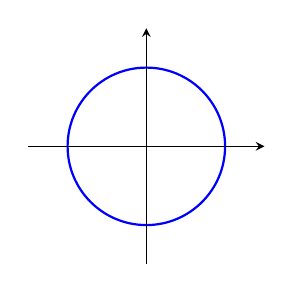
\begin{tikzpicture}
        \draw [blue, thick] (0,0) circle (1);
        \draw [-stealth] (-1.5, 0) -- (1.5, 0);
        \draw [-stealth] (0, -1.5) -- (0, 1.5);
    \end{tikzpicture}
    \end{center}
}
\begin{minipage}{\textwidth}
    \osservazione{
    Si noti come in questo esempio, 

    \vspace{0.5em}
    \begin{multicols}{2}
        \begin{align*}
        \frac{1}{2}&\to \frac{\sqrt{3}}{2}\\
        \frac{1}{2}&\to \frac{-\sqrt{3}}{2}
        \end{align*}
    \begin{center}
        \columnbreak

        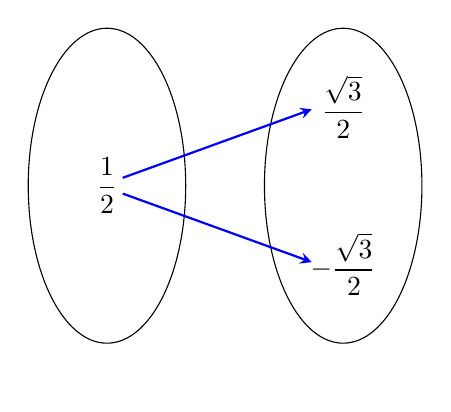
\begin{tikzpicture}
            \draw (-1.5,0) ellipse (1 and 2);
            \draw (1.5,0) ellipse (1 and 2);
            \node at (-1.5, -2.4) {$\R$};
            \node at (1.5, -2.4) {$\R$};
            \node at (-1.5, 0) {$\displaystyle%
            \frac{1}{2}$};
            \node at (1.5, 1) {$\displaystyle%
            \frac{\sqrt{3}}{2}$};
            \node at (1.5, -1) {$\displaystyle%
            -\frac{\sqrt{3}}{2}$};
            \draw [blue, thick, -stealth] (-1.3, 0.1) -- (1.1, 0.97); 
            \draw [blue, thick, -stealth] (-1.3, -0.1) -- (1.1, -0.97); 
        \end{tikzpicture}
    \end{center}
    \end{multicols}
    Mentre in altri casi, come \begin{align*}
    \mathscr{G} :\R & \to \R \\
    x & \mapsto x^{2}
    \end{align*} con \[
        \mathcal{R} =\{(x,y) \in \R^{2}\,|\, y=x^{2}\}
    \] vale \begin{equation}
        \forall\, x \in X=\R\quad \exists!\, y \in Y=\R\,\tc\, y=\mathscr{G} (x)\label{proprieta1}
    \end{equation}
}
\end{minipage}

\esempio{
    Sia $ X $ l'insieme dei fantini e $ Y $ l'insieme dei cavalli. $ Y= \mathscr{L}(x) $ se $ x  $ ha cavalcato almeno una volta $ y $. La corrispondenza può avere una forma simile:
    \begin{center}
        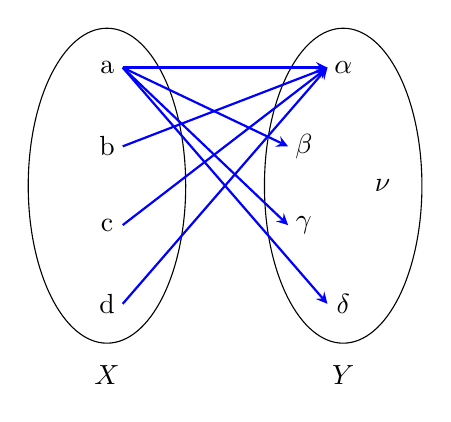
\begin{tikzpicture}
            \draw (-1.5,0) ellipse (1 and 2);
            \draw (1.5,0) ellipse (1 and 2);
            \node at (-1.5, -2.4) {$X$};
            \node at (1.5, -2.4) {$Y$};
            \node at (-1.5, 1.5) {a};
            \node at (-1.5, 0.5) {b};
            \node at (-1.5, -0.5) {c};
            \node at (-1.5, -1.5) {d};
            \node at (1.5, 1.5) {$\alpha$};
            \node at (1, 0.5) {$\beta$};
            \node at (1, -0.5) {$\gamma$};
            \node at (1.5, -1.5) {$\delta$};
            \node at (2, 0) {$\nu$};
            \draw [blue, thick, -stealth] (-1.3, 1.5) -- (1.3, 1.5); 
            \draw [blue, thick, -stealth] (-1.3, 1.5) -- (0.8, 0.5); 
            \draw [blue, thick, -stealth] (-1.3, 1.5) -- (0.8, -0.5); 
            \draw [blue, thick, -stealth] (-1.3, 1.5) -- (1.3, -1.5); 
            \draw [blue, thick, -stealth] (-1.3, 0.5) -- (1.3, 1.5); 
            \draw [blue, thick, -stealth] (-1.3, -0.5) -- (1.3, 1.5); 
            \draw [blue, thick, -stealth] (-1.3, -1.5) -- (1.3, 1.5); 
        \end{tikzpicture}
    \end{center}
    In questo caso la proprietà \eqref{proprieta1} non è soddisfatta.
}

Si nota che vi è una sostanziale differenza tra $ \mathscr{L} $ e $ \mathscr{G} $

\section{Funzioni}
\definizione{}{Una corrispondenza $ \mathscr{G} $:
    \begin{align*}
    \mathscr{G}: X & \to Y \\
     & x \mapsto y=\mathscr{G}(x)
    \end{align*} è una  textit{funzione} se $ \forall\,x \in X $ esiste al più un $ y \in Y $ tale che $ y=\mathscr{G}(x) $.
}

Nel corso si utilizzeranno sempre funzioni \begin{align*}
f:\R^{m} & \to \R^{n} \\
x & \mapsto y=f(x)
\end{align*}

\subsection{Definizioni}

\definizione{}{
    $ D \subseteq \R^{m} $ è detto \textit{dominio} di $ f $ se \[
        \forall\, x \in D\quad \exists\, y \in \R^{n}\,\tc\, y=f(x)
    \]

    Se non meglio specificato, $ D $ è dato da tutti gli $ x \in \R^{m} $ per cui l'espressione $ y =f(x) $ ha significato.
}
%DOMANDA: nella scrittura f:X\to Y, X è il dominio e Y è il codominio, vero? A questo punto, non è sbagliato scrivere log x: R\to R? Non andrebbe scritto log x: D\to R, specificando successivamente il dominio?
\definizione{}{Data una funzione \begin{align*}
f:X & \to Y \\
x & \mapsto y
\end{align*} si definisce \textit{codominio} di $ f $ l'insieme $ Y $.}
\esempio{}{
    $ f(x)=\ln (x-1) $, $ f: \R\to \R $. Deve valere $ x-1>0 $, pertanto \[
        D=(1, +\infty)=\{x \in \R\,|\, x>1\}
    \]
}
\notazione{}{
    Indichiamo \[
        D=\dom f
    \]
}
\esempio{}{
    Sia $ v=v(t) $ la velocità all'istante $ t $ di un corpo in caduta libera con velocità iniziale nulla.
    $ D \subseteq \R $ \begin{align*}
    v:D & \to \R \\
    t & \mapsto v(t)=g\,t
    \end{align*} con $ g $ accelerazione. Si noti che $ D\neq \R $, in quanto $ t $ è un tempo, e pertanto deve essere $ t\ge 0 $, allora \[
        D=[0, +\infty)=\{t \in \R; t\ge 0\}
    \]
}
\attenzione{Il dominio $ D=\dom f $ fa parte integrante della definizione della funzione, e deve essere sempre indicato.}
\esempio{}{\phantomsection\label{esempiofuncin}
        \begin{align*}
        f:\R &\to \R & g:[0; + \infty) &\to \R\\
        x & \mapsto y=x^{2} &  x &\mapsto y=x^{2}\\
        \dom f &= \R & \dom g &= [0; + \infty)
        \end{align*} 
        
        Si noti che \begin{align*}
            \graph (f)&=\{(x,y) \in \R\,|\, y=x^{2}\}\\ \graph (g)&=\{(x,y) \in [0; + \infty)\,|\, y=x^{2}\}
        \end{align*}

        $ f $ e $ g $ sono funzioni diverse.
}

\subsection{Funzioni iniettive, suriettive e biiettive}
\definizione{Data una funzione $ g:D\to Y $, $ f $ è \textit{iniettiva} se \begin{equation}
        \forall\,x_1, x_2 \in \dom g\qquad \begin{aligned}
            g(x_1)=g(x_2) \,&\implies\,x_1=x_2\\
            \big(x_1\neq x_2 \,&\implies\, g(x_1)\neq g(x_2)\big)
        \end{aligned}
    \end{equation}
}
\osservazione{}{
    La funzione $ g $ dell'\hyperref[esempiofuncin]{esempio (\thesection.\theesempi)} è iniettiva.
}
\definizione{}{
    Data $ f:D\to Y $, $ D=\dom f $, diciamo \textit{immagine} di $ f $ \begin{equation}
        f(D)=\im (f)=\bigl\{y \in Y\,\tc\quad \exists\, x \in D\,|\, y =f(x)\bigl\}
    \end{equation}
}
\definizione{}{
    Diciamo che \begin{align*}
    f:D & \to Y \\
    x & \mapsto f(x)
    \end{align*} è \textit{suriettiva} se \begin{equation}
        \forall\, y \in Y\quad \exists\, x \in D\,\tc\, y=f(x)
    \end{equation}
}

Una funzione $ f:D\to f(D) $ è sempre suriettiva.

\definizione{}{Diciamo che $ f: D\to Y $ è \textit{biettiva} (biunivoca) se è sia suriettiva che iniettiva.}

\subsection{Funzione composta}

Siano $ X, Y, W $ insiemi generici, e siano \begin{gather*}
    \begin{aligned}
        f: D &\to Y\\
        x &\mapsto y =f(x)
    \end{aligned}\qquad D=\dom f \subseteq X\\
    \begin{aligned}
        g: D' &\to w\\
        y &\mapsto w =g(x)
    \end{aligned}\qquad D'=\dom g \subseteq Y
\end{gather*}

Assumendo $ f(D) \subseteq D' $, possiamo costrure $ F $:
\begin{center}
    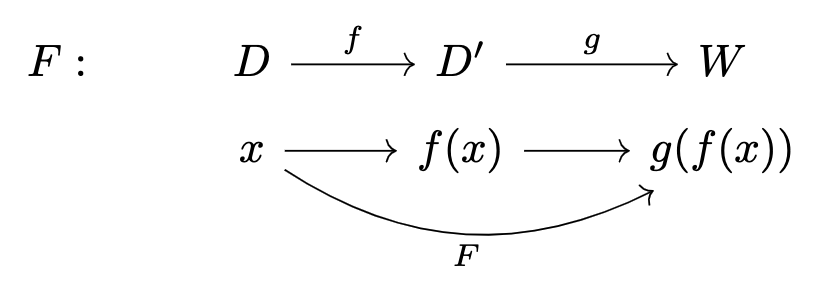
\includegraphics[width=7cm]{1.png}
\end{center}

La funzione \begin{align*}
F:D & \to W \\
x & \mapsto F(x)=g\bigl(f(x)\bigr)
\end{align*} è detta \textit{funzione composta} di $ f $ e $ g $. Si indica \[
    F=g\circ f
\]
\esempio{}{
    Siano $ D, D' \subseteq \R $, \[
        \begin{aligned}
            f: D&\to \R\\
            x &\mapsto x^{2}
        \end{aligned}\hspace{4em}\begin{aligned}
            g: D' &\to \R\\
            x&\mapsto \sqrt{x}
        \end{aligned}
    \]
    \vspace{1em}

    \begin{multicols}{2}
        \begin{center}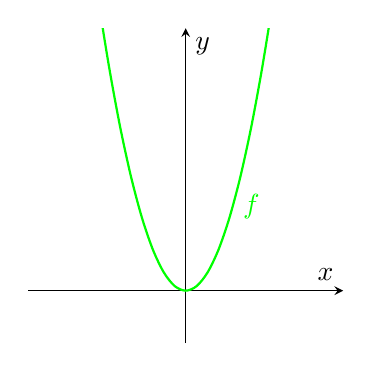
\begin{tikzpicture}\begin{axis}[
                xlabel=$x$,
                ylabel=$y$,
                axis equal,
                axis lines=middle,
                enlargelimits,
                xmax=5,
                xmin=-5,
                ymax=9,
                ymin=-1,
                xtick={0},
                ytick={0},
                scale only axis, 
                height=4cm, 
                width=4cm
                ]
            \addplot [no marks, green, smooth, thick, x=-1:5] {x^2};
            \node at (2.5, 3.2) {\textcolor{green}{$f$}};
        \end{axis}\end{tikzpicture}\end{center}
        \columnbreak

        \begin{center}
        \begin{tikzpicture}
            \begin{axis}[
                xlabel=$x$,
                ylabel=$y$,
                axis equal,
                axis lines=middle,
                enlargelimits,
                xmax=5,
                xmin=-1,
                ymax=5,
                ymin=-1,
                xtick={0},
                ytick={0},
                scale only axis, 
                height=4cm, 
                width=4cm
                ]
                \addplot [no marks, blue, smooth, thick, domain=0:5] {x^0.5};
                \node at (1, 1.6) {\textcolor{blue}{$g$}};
            \end{axis}
        \end{tikzpicture}\end{center}
    \end{multicols}
    

    Sia ha $ D=\dom f=\R $, $ D'=\dom g=[0, + \infty) $. Inoltre \[
        f(D)=[0, + \infty) \subseteq \dom g
    \] \begin{align*}
    g\circ f:\R & \to [0, + \infty) \\
    x & \mapsto \sqrt{x^{2}}=|x|
    \end{align*}

    Vale $ \dom f= \R $, $ \dom g=[0, + \infty) $, $ \dom (g\circ f)= \R $

    \begin{center}
    \begin{tikzpicture}
        \begin{axis}[
            xlabel=$x$,
            ylabel=$y$,
            axis equal,
            axis lines=middle,
            enlargelimits,
            xmax=5,
            xmin=-5,
            ymax=5,
            ymin=-1,
            xtick={0},
            ytick={0},
            scale only axis, 
            height=4cm, 
            width=6cm
            ]
            \addplot [no marks, red, smooth, thick, domain=-5:0] {-x};
            \addplot [no marks, red, smooth, thick, domain=0:5] {x};
            \node at (1, 2.3) {\textcolor{red}{$g\circ f$}};
        \end{axis}
    \end{tikzpicture}\end{center}
}   
\esempio{}{
    \[
        \begin{aligned}
            D& \subseteq \R^{2}\\
            f:D & \to \R^{2} \\
            x=(x_1,x_2) & \mapsto y=(x_1^{2},x_2^{2})
        \end{aligned}\qquad
        \begin{aligned}
            D'& \subseteq \R^{2}\\
            g:D' & \to \R \\
            x=(x_1,x_2) & \mapsto y=\sqrt{x_1+x_2}
        \end{aligned}
    \]
    Vale: $ D=\dom f=\R^{2} $ \[
        \im (f)=[0, + \infty)\times [0, + \infty)
    \]
    \begin{center}
        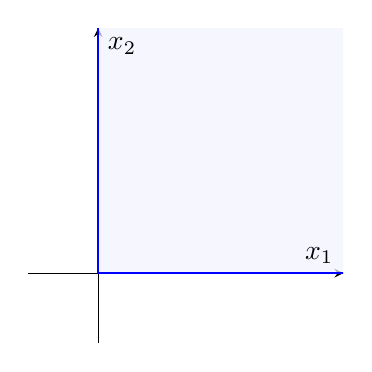
\begin{tikzpicture}
            \begin{axis}[
                xlabel=$x_1$,
                ylabel=$x_2$,
                axis equal,
                axis lines=middle,
                enlargelimits,
                xmax=5,
                xmin=-1,
                ymax=5,
                ymin=-1,
                xtick={0},
                ytick={0},
                scale only axis, 
                height=4cm, 
                width=4cm
                ]
                \addplot [no marks, blue, thick, fill=blue!5, fill opacity=0.7] coordinates {(0,0) (0,7) (7,7) (7, 0) (0,0)};
            \end{axis}
        \end{tikzpicture}\end{center}

        Inoltre \[
            D'=\dom g=\{(x_1, x_2) \in \R^{2}\,|\, x_1+x_2\ge 0\}
        \]
        \begin{center}
            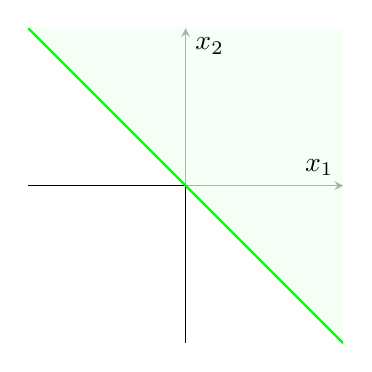
\begin{tikzpicture}
                \begin{axis}[
                    xlabel=$x_1$,
                    ylabel=$x_2$,
                    axis equal,
                    axis lines=middle,
                    enlargelimits,
                    xmax=5,
                    xmin=-5,
                    ymax=5,
                    ymin=-5,
                    xtick={0},
                    ytick={0},
                    scale only axis, 
                    height=4cm, 
                    width=4cm
                    ]
                    \addplot [no marks, green, thick, fill=green!5, fill opacity=0.7] coordinates {(-7,7) (7,-7) (7,7) (-7, 7)};
                \end{axis}
            \end{tikzpicture}\end{center}

            Quindi $ \im(f) \subseteq \dom g $ \begin{align*}
            g\circ f:\R^{2} & \to \R \\
            x=(x_1,x_2) & \mapsto \sqrt{x_1^{2}+x_2^{2}}=|x|
            \end{align*}
            \begin{center}
                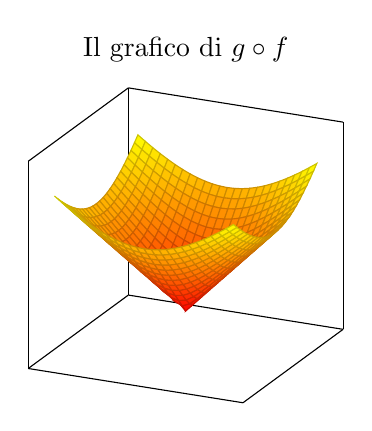
\begin{tikzpicture}
                    \begin{axis}[
                        xlabel=,
                        ylabel=,
                        zlabel=,
                        axis equal,
                        enlargelimits,
                        xmax=5,
                        xmin=-5,
                        ymax=5,
                        ymin=-5,
                        xtick=\empty,
                        ytick=\empty,
                        ztick=\empty,
                        scale only axis, 
                        height=4cm, 
                        width=4cm,
                        view={25}{20},
                        title={Il grafico di $ g\circ f $}
                        ]
                        \addplot3 [no marks, surf,
                        colormap/redyellow] ({x}, {y}, {(x^2 + y^2)^0.5});
                    \end{axis}
                \end{tikzpicture}\end{center}

}
\esempio{}{
    \[
        \begin{aligned}
            D& \subseteq \R\\
            f:D & \to \R \\
            x & \mapsto x^{2}
        \end{aligned}\hspace{3em}
        \begin{aligned}
            D'& \subseteq \R\\
            g:D' & \to \R \\
            x & \mapsto \ln x
        \end{aligned}
    \]
    Si ha $ D=\dom f=\R $, $ D'=\dom g =(0, + \infty) $

    \begin{multicols}{2}
        \begin{center}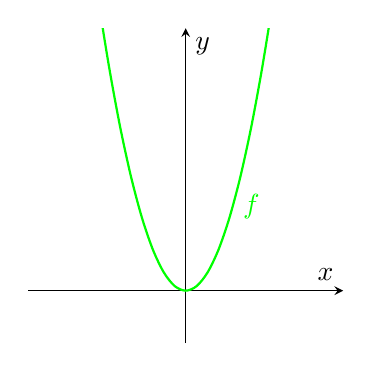
\begin{tikzpicture}\begin{axis}[
                xlabel=$x$,
                ylabel=$y$,
                axis equal,
                axis lines=middle,
                enlargelimits,
                xmax=5,
                xmin=-5,
                ymax=9,
                ymin=-1,
                xtick={0},
                ytick={0},
                scale only axis, 
                height=4cm, 
                width=4cm
                ]
            \addplot [no marks, green, smooth, thick, x=-1:5] {x^2};
            \node at (2.5, 3.2) {\textcolor{green}{$f$}};
        \end{axis}\end{tikzpicture}\end{center}
        \columnbreak

        \begin{center}
        \begin{tikzpicture}
            \begin{axis}[
                xlabel=$x$,
                ylabel=$y$,
                axis equal,
                axis lines=middle,
                enlargelimits,
                xmax=5,
                xmin=-1,
                ymax=5,
                ymin=-1,
                xtick={1},
                ytick={0},
                scale only axis, 
                height=4cm, 
                width=4cm
                ]
                \addplot [no marks, blue, smooth, thick, domain=0:5] {ln(x)};
                \node at (3, 1.7) {\textcolor{blue}{$g$}};
            \end{axis}
        \end{tikzpicture}\end{center}
    \end{multicols}

    Dal momento che $ f(D)=[0, + \infty) \nsubseteq D' $ non possiamo costruire $ g \circ f $. Restringiamo $ f $: \begin{align*}
    \tilde{f}:\R\setminus\{0\} & \to \R \\
    x & \mapsto x^{2}
    \end{align*} $ \tilde{f}(D)=(0,+ \infty) \subseteq\dom g $ \begin{align*}
    g\circ\tilde{f}:\R\setminus\{0\} & \to \R \\
    x & \mapsto \ln(x^{2})
    \end{align*}

    \begin{center}
        \begin{tikzpicture}
            \begin{axis}[
                xlabel=$x$,
                ylabel=$y$,
                axis equal,
                axis lines=middle,
                enlargelimits,
                xmax=5,
                xmin=-5,
                ymax=5,
                ymin=-1,
                xtick={0},
                ytick={0},
                scale only axis, 
                height=4cm, 
                width=6cm
                ]
                \addplot [no marks, red, unbounded coords=jump, thick] {ln(x^2)};
                \node at (1.4, 2.3) {\textcolor{red}{$\ln(x^{2})$}};
            \end{axis}
        \end{tikzpicture}\end{center}
}
\subsection{Funzione inversa}

Siano $ X, Y $ insiemi generici, $ D \subseteq X $. Se $ f:D\to Y $ è iniettiva, allora \[
    f:D\to f(D)
\] è \textit{biunivoca}, ovvero \begin{equation}
    \forall\,y \in f(D)\quad \exists!\, x \in D\quad y=f(x)
\end{equation}

Diciamo che $ f $ tra $ D $ e $ f(D) $ è \textit{invertibile}. Diciamo \textit{funzione inversa} di $ f $ \begin{align*}
\varphi:f(D) & \to D \\
y & \mapsto \varphi(y)=x
\end{align*} dove $ x $ è l'unico elemento di $ D $ tale che $ y=f(x) $. Si ha allora 
\[
    \begin{aligned}
        \varphi\circ f: D&\to D\\
        \dom f&\to \dom f\\
        x &\mapsto \varphi\circ f(x)=x
    \end{aligned}\hspace{4em}\begin{aligned}
        f\circ\varphi: f(D) &\to f(D)\\
        y&\mapsto f\circ\varphi(y)=y
    \end{aligned}
\] ossia \begin{equation}
    \varphi \circ f =\Id_{D} \qquad f\circ\varphi = \Id_{f(D)} 
\end{equation} dove $ \Id_{D}  $ è l'identità in $ D $ e $ \Id_{f(D)}  $ è l'identità in $ f(D) $.

La funzione inversa $ \varphi $ in genere si indica con $ f^{-1} $: \[
    f^{-1} \circ f =\Id_{D} \qquad f\circ f^{-1} = \Id_{f(D)}
\]
\esempio{}{
    \begin{align*}
    f:[0, + \infty) & \to [0, + \infty) \\
    x & \mapsto x^{2}
    \end{align*} $ \dom f =[0, + \infty) $: $ f  $ è biunivoca e dunque invertibile \begin{align*}
    f^{-1}:[0, + \infty) & \to [0, + \infty) \\
    x & \mapsto f^{-1}(x)= \sqrt{x}
    \end{align*}

    \begin{multicols}{2}
        \begin{center}\begin{tikzpicture}\begin{axis}[
                xlabel=$x$,
                ylabel=$y$,
                axis equal,
                axis lines=middle,
                enlargelimits,
                xmax=5,
                xmin=-5,
                ymax=9,
                ymin=-1,
                xtick={0},
                ytick={0},
                scale only axis, 
                height=4cm, 
                width=4cm
                ]
            \addplot [no marks, green, smooth, thick, domain=0:5] {x^2};
            \node at (2.5, 3.2) {\textcolor{green}{$f$}};
        \end{axis}\end{tikzpicture}\end{center}
        \columnbreak

        \begin{center}
        \begin{tikzpicture}
            \begin{axis}[
                xlabel=$x$,
                ylabel=$y$,
                axis equal,
                axis lines=middle,
                enlargelimits,
                xmax=5,
                xmin=-1,
                ymax=5,
                ymin=-1,
                xtick={0},
                ytick={0},
                scale only axis, 
                height=4cm, 
                width=4cm
                ]
                \addplot [no marks, blue, smooth, thick, domain=0:5] {x^0.5};
                \node at (1, 1.6) {\textcolor{blue}{$g$}};
            \end{axis}
        \end{tikzpicture}\end{center}
    \end{multicols}
    \begin{gather*}
        f^{-1}\circ f (x) = \sqrt{x^{2}}= x \qquad x\ge 0\\
        f \circ f^{-1}(x) = (\sqrt{x})^{2} = x\qquad x\ge 0
    \end{gather*}
}
\attenzione{
    Non confondere la funzione \textit{inversa} $ f^{-1} $ (ovvero tale che $f^{-1}\circ f =\id_{D} $) con la funzione \textit{reciproca} 
    \[
        [f(x)]^{-1}=\frac{1}{f(x)}
    \]
}

Nell'esempio precedente, funzione inversa e funzione reciproca sono ben diverse. Infatti, data \begin{align*}
f:[0,+ \infty) & \to [0, + \infty) \\
x & \mapsto x^{2}
\end{align*} vale che \[
    f^{-1}(x)=\sqrt{x}\qquad f(x)^{-1}=\frac{1}{x^{2}}
\] inoltre \[
    f \circ f^{-1}(x)=x\qquad f(x) \cdot f(x)^{-1}=1 \quad\forall\, x \in \R\setminus\{0\}
\]

\subsubsection{Grafico della funzione inversa}

\begin{center}
    \begin{tikzpicture}
        \begin{axis}[
            xlabel=$x$,
            ylabel=$y$,
            axis equal,
            axis lines=middle,
            enlargelimits,
            xmax=5,
            xmin=-1,
            ymax=5,
            ymin=-1,
            xtick={1},
            ytick={1},
            scale only axis, 
            height=7cm, 
            width=7cm,
            title={$f(x)=x^{2}\qquad x\ge 0$}
            ]
            \addplot [no marks, red, smooth, thick, domain=0:5] {x^0.5};
            \node at (4, 1.6) {\textcolor{red}{$f^{-1}(x)$}};
            \addplot [no marks, blue, smooth, thick, domain=0:5] {x^2};
            \node at (1.5, 4) {\textcolor{blue}{$f(x)$}};
            \addplot [no marks, green, dashed, thick] coordinates {(-3,-3) (7,7)};
        \end{axis}
    \end{tikzpicture}\end{center}

Il grafico di $ f^{-1} $ è il simmetrico del grafico di $ f $ rispetto alla bisettrice del primo e del terzo quadrante.

\esercizio{
    Verificare che la funzione $ f(x)=\sin x $ sia invertibile su $ \bigl[-\frac{\pi}{2}, +\frac{\pi}{2}\bigr] $, determinare il dominio dell'inversa e disegnare entrambi i grafici \[
        f^{-1}(x)=\arcsin x
    \]
}{
    Da risolvere %ESERCIZIO risolvere esercizio
}{}
\esercizio{
    Verificare che la funzione $ g(x)=\tan x $ è invertibile su $ \bigl(-\frac{\pi}{2}, +\frac{\pi}{2}\bigr) $, determinare dominio e grafico di $ g^{-1}(x) $ \[
        g^{-1}(x)=\arctan x
    \]
}{
    Da risolvere %ESERCIZIO risolvere esericizio
}{}

\subsection{Funzioni limitate}

Dato $ D \subseteq \R^{n} $,\begin{align*}
f:D & \to \R \\
x & \mapsto f(x)
\end{align*} è detta \textit{limitata} se $ f(D) $ è un insieme limitato, ossia \[
    \exists\, M>0\,\tc\quad \forall\, x \in D\qquad \begin{aligned}
        |f(x)|&<M\\
        -M<f(x)&< M
    \end{aligned}
\]

$ f $ è limitata superiormente (inferiormente) se \[
    \exists\, M>0\,\tc\quad \forall\, x \in D\qquad\begin{aligned}
        f(x)&<M\\
        \bigl(f(x)&>-M\bigr)
    \end{aligned}
\]

\esempio{}{
    \begin{align*}
    f:\R & \to \R \\
    x & \mapsto \sin x
    \end{align*} $ f $ è limitata in quanto $ f(D) \subseteq [-1, 1] $, ovvero \[
        \forall\, x \in \R\qquad -1\le f(x)\le 1
    \]
    \begin{center}
        \begin{tikzpicture}
            \begin{axis}[
                xlabel=$x$,
                ylabel=$y$,
                axis equal,
                axis lines=middle,
                enlargelimits,
                xmax=8,
                xmin=-8,
                ymax=2,
                ymin=-2,
                xtick={0},
                ytick={-1, 1},
                scale only axis, 
                height=4cm, 
                width=10cm]
                \addplot [no marks, blue, thick, samples=1000, domain=-8:8] {sin(x*180/3.1415)};
                \addplot [no marks, red, dashed, thick, domain=-8:8] {1};
                \addplot [no marks, red, dashed, thick, domain=-8:8] {-1};
            \end{axis}
        \end{tikzpicture}\end{center}
}
\definizione{}{
    Data $ f:D\to \R $, con $ D \subseteq \R $, diciamo \textit{estremo superiore} (inferiore) di $ f $ su $ D $ 
    \begin{align}
        \sup_{D} f &:= \sup\bigl(f(D)\bigr)\\
        \Bigl(\inf_{D} f &:= \inf\bigl(f(D)\bigr) \Bigr)
    \end{align} 
}
\esempio{Ecco due funzioni:

\begin{minipage}{\textwidth}
    \begin{multicols}{2}
        \begin{center}\begin{tikzpicture}\begin{axis}[
                xlabel=$x$,
                ylabel=$y$,
                axis equal,
                axis lines=middle,
                enlargelimits,
                xmax=5,
                xmin=-5,
                ymax=5,
                ymin=-5,
                xtick={0},
                ytick={0},
                scale only axis, 
                height=4cm, 
                width=4cm
                ]
            \addplot [no marks, green, smooth, thick, domain=-5:5] {x^3};
        \end{axis}\end{tikzpicture}\end{center} \begin{align*}
        f:\R & \to \R \\
        x & \mapsto x^{3}
        \end{align*}

        $ f $ non è limitata.
        \columnbreak

        \begin{center}
        \begin{tikzpicture}
            \begin{axis}[
                xlabel=$x$,
                ylabel=$y$,
                axis equal,
                axis lines=middle,
                enlargelimits,
                xmax=5,
                xmin=-1,
                ymax=5,
                ymin=-1,
                xtick={0},
                ytick={0},
                scale only axis, 
                height=4cm, 
                width=4cm
                ]
                \addplot [no marks, blue, smooth, thick, domain=0:5] {x^3};
\end{axis}\end{tikzpicture}\end{center}
\begin{align*}
g:[0,+\infty) & \to \R \\
x & \mapsto x^{3}
\end{align*} 

$ g $ è limitata inferiormente, e \[\inf_{[0,+ \infty)}  g =0=\min_{[0,+ \infty)}  g\]
\end{multicols}\end{minipage}}

\definizione{}{
    $ \sup f $ e $ \inf f$, se appartengono all'immagine $ f(D) $ sono detti \textit{valore massimo} e \textit{minimo} di $ f $.
}

\subsection{Massimi, minimi e monotonia}

Data $ f:D\to \R $, $ D \subseteq \R^{n} $, 
\begin{itemize}
\item $ x_0 \in D $ è \textit{punto di massimo} (\textit{minimo}) \textit{assoluto} o globale di $ f $ se \begin{equation}
    \forall\, x \in D\qquad \begin{aligned}
        f(x)&\le f(x_0)\\
        \bigl(f(x)&\ge f(x_0)\bigr)
    \end{aligned}
\end{equation}
\item $ x_0 $ è detto \textit{punto di massimo} (\textit{minimo}) \textit{locale} o relativo di $ f $ se \begin{equation}
    \exists\, U(x_0)\,\tc\quad \forall\, x \in U(x_0)\quad \begin{aligned}
        f(x)&\le f(x_0)\\
        \bigl(f(x)&\ge f(x_0)\bigr)
    \end{aligned}
\end{equation}
\item $ x_0 $ è detto \textit{punto di massimo} (\textit{minimo}) \textit{forte} di $ f $ se \begin{equation}
    \begin{aligned}
        \forall\, x &\in D\\
        \bigl(\exists\, U(x_0)\,\tc\quad \forall\, x &\in U(x_0)\bigr)
    \end{aligned}\qquad
     x\neq x_0\text{ si ha}\quad \begin{aligned}
        f(x)&< f(x_0)\\
        \bigl(f(x)&> f(x_0)\bigr)
    \end{aligned}
\end{equation}
\end{itemize}

\subsubsection{Funzioni monotone}   

Data $ f:D\to \R $, $ D \subseteq \R^{n} $, 
\begin{itemize}
\item $ f $ è \textit{crescente} (\textit{decrescente}) su $D $ se \begin{equation}
    \forall\, x_1, x_2 \in D\qquad x_1<x_2 \,\implies\, \begin{aligned}
        f(x_1)&\le f(x_2)\\
        \bigl(f(x_1)&\ge f(x_2)\bigr)
    \end{aligned}
\end{equation}
\item $ f $ è \textbf{strettamente} \textit{crescente} (\textit{decrescente}) su $D $ se \begin{equation}
    \forall\, x_1, x_2 \in D\qquad x_1<x_2 \,\implies\, \begin{aligned}
        f(x_1)&< f(x_2)\\
        \bigl(f(x_1)&> f(x_2)\bigr)
    \end{aligned}\end{equation}
\end{itemize}
Sia $V$ spazio vettoriale di dimensione finita, $V=W_1+W_2$ con $W_1$, $W_2$ sottospazi vettoriali $\implies$ 
\[\dim V = \dim W_1 + \dim W_2 - \dim (W_1 \cap W_2)\]
In particolare se $ W_1 \cap W_2 = \{\underline{0}\}$ , allora
\[V=W_1 \oplus W_2 \,\implies\, \dim V = \dim W_1 + \dim W_2\]
    
\esercizio{
    Sia $V=R^4$, 
    \begin{align*}
        W_1&=\{(x_1, x_2, x_3, x_4)\,|\,2x_1 - x_2 + x_3 = 0, x_1+x_2-x_4=0\}\\
        W_2&= \mathscr{L}\left((0,0,1,1), (1,1,0,0), (2,2,-2,-2)\right)
    \end{align*}
    \begin{enumerate}
        \item Si trovino una base di $ W_1 $ e una base di $ W_2 $.
        \item Si calcoli $\dim (W_1+W_2)$ e si dica se la somma è diretta.
        \item Si scriva $(2, 1, -1, 1)$ come somma di un vettore in $ W_1 $ con un vettore in $ W_2 $.
    \end{enumerate}
}{
    \begin{enumerate}
        \item $ W_1 $ è formato dai vettori $x=(x_1, x_2, x_3, x_4)$ le cui componenti risolvono questo sistema
        \[
        \begin{cases}
        2x_1-x_2+x_3=0\\
        x_1+x_2-x_4=0
        \end{cases} \,\implies\, 
        \begin{cases}
        x_1=t\\
        x_2=s\\
        x_3=-2+s\\
        x_4=t+s
        \end{cases}
        \]
        \[
            \begin{pmatrix}
                x_1\\ x_2\\ x_3\\ x_4
            \end{pmatrix}= t\,\begin{pmatrix}
                1\\ 0\\ -2\\ 1
            \end{pmatrix}+s\,\begin{pmatrix}
                0\\ 1\\ 1\\ 1
            \end{pmatrix}
        \] 
        
        $\implies$ $W_1= \mathscr{L}\left((1, 0, -2, 1), (0, 1, 1, 1)\right)$, ma i due generatori sono linearmente indipendenti 
        
        $\implies$ $ \mathscr{B}_1=\{(1,0,-2,1),(0,1,1,1)\}$ base di $ W_1 $, con $v_1=(1,0,-2,1)$ e $v_2=(0,1,1,1)$
    
        Per $ W_2 $ si osserva che \[(2, 2, -2, -2)=-2(0,0, 1, 1)+2(1, 1, 0, 0)\] 
        
        $\implies$ $W_2= \mathscr{L}\left((0,0,1,1), (1, 1, 0, 0)\right)$. 
        
        Poiché i due generatori sono linearmente indipendenti 
        
        $\implies$ $ \mathscr{B}_2=\{(0,0,1,1),(1,1,0,0)\}$ base di $ W_2 $, con $w_1=(0,0,1,1)$ e $w_2=(1,1,0,0)$.
        \item $W_1+W_2$ contiene $v_1, v_2, w_1, w_2$, so che $ \mathscr{B}_1=\{v1,v2\}$ è libero. 
        
        Considero $\{v1, v2, w1\}$ e mi chiedo se è libero, quindi studio il sistema $w_1=\lambda\, v_1 + \mu\, v_2$
        \[
            \begin{pmatrix}
                0\\ 0\\ 1\\ 1
            \end{pmatrix} = \lambda \begin{pmatrix}
                1\\ 0\\ -2\\ 1
            \end{pmatrix} + \mu \begin{pmatrix}
                0\\ 1\\ 1\\ 1 
            \end{pmatrix}= \begin{pmatrix}
                \lambda \\ \mu\\ -2\lambda + \mu\\ \lambda+\mu
            \end{pmatrix} \,\implies\, \begin{cases}
                \lambda=0\\
        \mu=0\\
        0=1\\
        0=1
            \end{cases}
        \] 
        
        $\implies$ il sistema non ha soluzione, $\{v_1, v_2, w_1\}$ è libero
        
        Considero $\{v_1, v_2, w_1, w_1\}$ e mi chiedo se è libero, quindi studio il sistema \[
            w_2=\lambda_1\,v_1 + \lambda_2\,v_2 + \lambda_3\,w_1
        \]
        \begin{multline*}
            \begin{pmatrix}
                1\\ 1\\ 0\\ 0
            \end{pmatrix}=\lambda_1 \begin{pmatrix}
                1\\ 0\\ -2\\ 1
            \end{pmatrix}+\lambda_2 \begin{pmatrix}
                0\\1\\1\\1
            \end{pmatrix}+\lambda_3 \begin{pmatrix}
                0\\0\\1\\1
            \end{pmatrix}=\\=\begin{pmatrix}
                \lambda_1\\ \lambda_2\\-2\lambda_1+\lambda_2+\lambda_3\\ \lambda_1+\lambda_2+\lambda_3
            \end{pmatrix} \,\implies\,
            \begin{cases}
                \lambda_1=1\\
                \lambda_2=1\\
                -1+\lambda_3=0 \,\implies\, \lambda_3=1\\
                2+\lambda_3=0 \,\implies\, \lambda_3=-2
            \end{cases}
        \end{multline*}

        Il sistema non ha soluzione e $\{v_1, v_2, w_1, w_2\}$ è libero 
        
        $\implies$ $W_1+W_2=\R^4$, per la formula di Grassmann $W_1 \cap W_2=\{\underline{0}\}$
        
        $\implies$ $R^4=W_1 \oplus W_2$ e $\{v_1, v_2, w_1, w_2\}$ è base di $\R^4$.
        \item Voglio scrivere $v=(2, 1, -1, 1)$ come $v=a+b$ con $a \in W_2$ e $b \in W_2$
        \[
        v=\lambda_1 v_1+ \lambda_2 v_2+ \mu_1 w_1 + \mu_2 w_2\] con $\lambda_1, \lambda_2, \mu_1, \mu_2$ unici, poiché $\{v_1, v_2, w_1, w_2\}$ base di $\R^4$. So che $\lambda_1 v_1 + \lambda_2 v_2 \in W_1$ e $\mu_1 w_1 + \mu_2 w_2 \in W_2$
        \[
            \begin{pmatrix}
                2\\ 1\\ -1 \\ 1
            \end{pmatrix} = \begin{pmatrix}
                \lambda_1\\ 0\\ -2\lambda_1\\ \lambda_1
            \end{pmatrix} + \begin{pmatrix}
                0\\ \lambda_2\\ \lambda_2\\ \lambda_2
            \end{pmatrix} + \begin{pmatrix}
                0\\ 0\\ \mu_1\\ \mu_1
            \end{pmatrix} + \begin{pmatrix}
                \mu_2\\ \mu_2\\ 0\\ 0
            \end{pmatrix}
        \] 
        \[
            \implies\,\begin{cases}
                \lambda_1+\mu_2=2\\
                \lambda_2+\mu_2=1\\
                -2\lambda_1+\lambda_2+\mu_1=-1\\
                \lambda_1+\lambda_2+\mu_1=1
            \end{cases} \,\implies\, \begin{cases}
                \lambda_1=2-\mu_2\\
                \lambda_2=1-\mu_2\\
                -4+2\mu_2+1-\mu_2+\mu_1=-1\\
                2-\mu_2+1-\mu_2+\mu_1=1
            \end{cases}
        \]
        \[
        \begin{cases}
            \lambda_1=2-\mu_2 \,\implies\, \lambda_1=\frac{2}{3}\\
            \lambda_2=1-\mu_2 \,\implies\, \lambda_2 = -\frac{1}{3}\\
            \mu_1+\mu_2=2 \,\implies\, \mu_1=2-\mu_2 \,\implies\, \mu_1=2-\frac{4}{3}=\frac{2}{3}\\
            \mu_1-2\mu_2=-2 \,\implies\, 2-\mu_2-2\mu_2=-2 \,\implies\, \mu_2=\frac{4}{3}
        \end{cases}
        \]
      
        $v=\frac{2}{3} v_1-\frac{1}{3} v_2+\frac{2}{3} w_1+\frac{4}{3} w_2$ 
        
        $\implies$ $a=\frac{2}{3} v_1-\frac{1}{3} v_2 \in W_1$ e $b=\frac{2}{3} w_1+\frac{4}{3} w_2 \in W_2$
    \end{enumerate}
}{}

\esercizio{
    Sia \[W=\{(x_1, x_2, x_3) \in \R^3 \,|\: x_1-x_2+x_3=0\}.\] Si trovino due sottospazi $W_1, W_2 \in \R^3$ con \[W_1 \neq W_2 \,|\: \R^3=W \oplus W_1,\: \R^3=W \oplus W_2\]

    Dal punto di vista geometrico $W$ è un piano nello spazio, mentre $ W_1 $ e $ W_2 $ sono due rette, passanti per l'origine, che non appartengano al piano.
}{
    $\dim W=2$, quindi $\dim W_1 = \dim W_2 = 1$

    Risulta $W_1= \mathscr{L}(w_1), W_2= \mathscr{L}(w_2)$, con $w_2, w_2\neq \underline{0}$, $ w_1 $, $ w_2 $ non paralleli e $w_1, w_2 \notin W$
    \begin{align*}
    w_1=(1, 1, 1) \notin W \,\implies\, W_1= \mathscr{L}(w_1):&\text{ risulta }\R^3=W \oplus W_1\\
    w_2=(3, 1, 1) \notin W \,\implies\, W_2= \mathscr{L}(w_2):&\text{ risulta }\R^3=W \oplus W_2
    \end{align*}
    Inoltre w1 e w2 non sono paralleli implies W1 neq W2
}{}

    
\section{Matrici II}
\subsection{Rango di una matrice e algoritmo di Gauss}
    
Sia $A \in \K^{m,n}$ con $\K$ campo. 
\[A=\begin{pmatrix}
    R_1\\ \vdots\\ R_m
\end{pmatrix}\]
dove $R_1, \cdots, R_m$ sono le righe di $A$.

Ogni riga ha $n$ componenti, e può essere identificata con un elemento in $\K^n$, quindi $R_1, R_2, \cdots, R_m \in \K^n$

$ \mathscr{L}(R_1,\cdots,R_m)$ è sottospazio vettoriale di $\K^n$

Quando modifico la matrice $A$ implementando le tre operazioni dell'algoritmo di Gauss trovo una nuova matrice, 
\[A'=\begin{pmatrix}
    R_1'\\ \vdots\\ R_m'
\end{pmatrix}\] 
ma per la natura delle operazioni \[ \mathscr{L}(R_1',\cdots,R_m')= \mathscr{L}(R_1,\cdots,R_m)\] se $A'$ è ridotta per righe, le righe non nulle di $A'$ sono una base di $ \mathscr{L}(R_1,\cdots,R_m) $.

\proposizione{}{
    Il rango di una matrice è la dimensione del sottospazio vettoriale generato dalle righe. Denoto
    \begin{equation}
        R(A):= \mathscr{L}(R_1,...,R_m)\subseteq \K^n, \dim R(A)=\rank(A)
    \end{equation}
}

Data $A \in \K^{m,n}$, 
\begin{equation*}
    A=\begin{pmatrix}
        R_1\\ \vdots\\ R_m
    \end{pmatrix}
\end{equation*}
dove $R_1, \cdots, R_m \in \K^n$ sono le righe della matrice; \begin{equation*}
    A=\begin{pmatrix}
        C_1 & \cdots & C_n
    \end{pmatrix}
\end{equation*} dove $C_1, \cdots, C_n$ sono le colonne di $A$, $C_1, \cdots,C_n \in \K^m$
\[
    R(A)= \mathscr{L}(R_1,...,R_m), \rank A=\dim R(A)
\]
Sia 
\[C(A):= \mathscr{L}(C_1,\cdots,C_n)\] sottospazio vettoriale di $\K^n$.
$C(A)=R(\null^t\!A)$ poiché per definizione di matrice trasposta le righe di $\null^t\!A$ sono le colonne di $A$.

\teorema[(del rango)]{rankequellleoijdafliygkjygjhgfjhgfjhgfjhgfcjghgffgfgffgfgfgfg}{
    Sia $A \in \K^{m,n}$ allora
    \begin{gather*}
        \rank(A) = \rank(\null^t\!A)\\
        \iff\\ 
        \dim R(A) = \dim C(A)
    \end{gather*}
}
\dimostrazione{rankequellleoijdafliygkjygjhgfjhgfjhgfjhgfcjghgffgfgffgfgfgfg}{
    Data $A \in \K^{m,n}$ e $R(A), C(A)$, siano $l=\dim C(A)$, $h=\dim R(A)$. Si dimostra che $l\le h$ e $h\le l$ 
    
    $\implies$ $l=h$.

    Sia $ \mathscr{B}=\{w_1, \cdots, w_h\}\subseteq \K^n$ una base di $R(A)$. Per ogni $R_i\in \mathscr{L}(w_1, \cdots, w_h)$ possiamo scrivere 
    \[R_i=b_{i1}\,w_1+b_{i2}\,w2+\cdots+b_{ih}\,w_h=\sum_{j=1}^h b_{ij}\,w_j\] per qualche $b_{i1}, \cdots, b_{ih} \in \K$

    Sia $D$ la matrice le cui righe sono i vettori $w_1, \cdots, w_h$, \[
        D=\begin{pmatrix}
            w_1\\ \vdots\\ w_k
        \end{pmatrix} \in \K^{h,n}
    \]
    Sia $B$ la matrice la cui entrata ($ij$)-esima è $b_{ij}$, $B \in \K^{m, h}$.

    Sappiamo che $R_i=\sum_{j=1}^h b_{ij}\,w_j$ 
    
    $\implies$ $A=BD$ $\implies$ $ \null^{t}\!A=\null^{t}\!D\,\null^{t}\!B $

    Le righe di $ \null^{t}\!A $ sono le colonne di $A$ 
    
    $\implies$ ogni colonna di $A$ è combinazione lineare degli stessi $h$-vettori  
    
    $\implies$ $\dim C(A)\le h$ $\implies$ $l\le h$

    Per dimostrare che $h\le l$ si applica lo stesso ragionamento partendo da $ \null^{t}\!A $, e concludendo che ogni riga di $A$ è combinazione lineare degli stessi $l$-vettori da cui segue $h\le l$.\qed
}

Se ne deduce che l'algoritmo di Gauss può essere implementato sulle colonne. Data $A \in \K^{m,n}$, le tre operazioni possono essere operate sulle colonne.
    
\teorema[(di nullità più rango)]{nullitrasoijfdsoirango}{
    Sia $A \in \K^{m,n}$, e si consideri il sistema lineare omogeneo associato $AX=\underline{0}$, con $X \in \K^{n}$.

    Sia $N(A)=\{X \in \K^n\, |\: AX=\underline{0}\}$ (nullspace di $A$), $N(A) \subseteq \K^n$ sottospazio vettoriale.

    Vale
    \begin{equation}
        \dim N(A) = n - \rank(A)
    \end{equation}
}
\dimostrazione{nullitrasoijfdsoirango}{
    $N(A)$ non cambia se sostituisco $A$ con una matrice ridotta per righe tramite l'algoritmo di Gauss. 
    
    Possiamo supporre $A$ ridotta per righe. $\rank(A)$ è il numero di righe di $A$, e sappiamo che le soluzioni del sistema $AX=\underline{0}$ dipendono da $n-r$ parametri.
    
    $\implies$ $\dim N(A)=n-r=n-\rank(A)$\qed
}
\includepdf[pages={1-}, addtotoc={
    1, subsection, 2, Funzioni senza limite, 12pi,
    1, subsection, 2, Proprietà dei limiti, 12pii
}]{PDF/202110120850.pdf} %12 ott
\includepdf[pages={1-}, %
addtotoc={
    1, subsection, 2, Algebra dei limiti, 18pi,
    3, subsection, 2, Algebra estesa dei limiti, 18pii,
    5, subsection, 2, Teoremi sui limiti, 18piii
}%
]{PDF/202110181045.pdf} %18 ott
\includepdf[pages={1-}, addtotoc={
    3, subsection, 2, Potenze ad esponente reale, 19pi,
    4, subsection, 2, Limiti notevoli e forme indeterminate, 19pii
}]{PDF/202110190840.pdf} %19 ott
\includepdf[pages={1-}, addtotoc={
    1, subsection, 2, Infiniti ed infinitesimi, 25pi,
    1, subsubsection, 3, Confronto di infinitesimi, 25pii,
    2, subsubsection, 3, Confronto di infiniti, 25piii,
    4, subsubsection, 3, Proprietà per infiniti e infinitesimi, 25piv
}]{PDF/202110251030.pdf} %25 ott
\includepdf[pages={1-}, addtotoc={
    1, subsection, 2, Altri limiti notevoli, 26pi,
    3, section, 1, Successioni, 26pii
}]{PDF/202110260852.pdf} %26 ott
\marginnote{2 nov 2021}

\section{Limite successione}

Data $ \{a_{n} \}_{n=0}^\infty, \N \to \R, a: n\to a_{n}  $, $l \in \R*$, diciamo che 
\[
    \lim_{n\to\infty}a_{n}=l  
\]
se $\forall V(l) \exists U(+\infty) n \in(\N intersezione D) \implies a_{n \in V(l)}$
Scriviamo $\forall V(l) \exists n_{segnato} \in N | \forall n>n_{segnato} a_{n} \in V(l)$

$l\in \R$, diciamo che $ \{a_{n} \}_{n=0}^\infty $ è \textbf{convergente} a $ l $ se $ \forall \varepsilon \exists n_{segnato} \in \N | \forall n>n_{segnato} |a_{n} -l |<\varepsilon  $

Se $ l=\pm \infty $ $a_{n}$ è divergente a $ \pm\infty $, se $ \lim_{n\to+\infty} a_{n}=\nexists $ allora $ \{a_{n}\}_{n=0 }^\infty$ è irregolare (o oscillante).


\esempio{
\begin{itemize}
    \item $ \{a_{n} \}_{n=0}^\infty=(-1)^n $ con $ n \in \N $ è irregolare e limitata
    \item $ \{b_{n} \}_{n=0}^\infty=(-1)^n\cdot n $ con $ n = 0, -1, 2, -3, 4, \cdots$ è irregolare e non limitata
\end{itemize}
}

Si dice di una successione $\{a_{n} \}_{n=0}^\infty$

\begin{itemize}
    \item $\forall \{a_{n} \}$ è crescente se $ \forall n \in \N $, $ a_{n} \le a_{n+1}  $
    \item $\forall\{a_{n} \}$ è strettamente crescente se $ \forall n \in \N $, $ a_{n} < a_{n+1}  $
    \item $\forall\{a_{n} \}$ è decrescente se $ \forall n \in \N $, $ a_{n} \ge a_{n+1}  $
    \item $\forall \{a_{n} \}$ è strettamente decrescente se $ \forall n \in \N $, $ a_{n} > a_{n+1}  $
\end{itemize}
Una successione crescente o decrescente si dice monotona, se strettamente crescente o decrescente si dice strettamente monotona.

Un predicato $ P(n) $ è verificato definitivamente se $ \exists n_{segnato} \forall n\le n_{segnato}$ $ P(n) $  è vero

Valgono per $ \{a_{n} \}_{n=0}^\infty$ i seguenti teoremi
\begin{itemize}
    \item Teorema di unicità del Limite
    \item Teorema di permanenza del segno 
    \item Teorema di limitatezza:
        \teorema{limitatezza}{
            \[
                \lim_{n\to \infty} a_{n} =l \in \R \,\implies\, \{a_{n} \}_{n=0}^\infty\text{ è convergente e limitata}
            \]
        }
    \item Teorema del confronto
    \item Teorema di esistenza del Limite per successioni definitivamente monotone
        \teorema{esistenzalim}{
            $ \{a_{n} \}_{n=0}^\infty $ è definitivamente crescente 
            
            $\implies$ ammette limite in $ \R* $

            Precisamente se 
            \begin{itemize}
                \item $\{a_{n} \}_{n=0}^\infty$ è definitivamente monotona e limitata 
            
                $\implies$ è convergente
                \item $ \{a_{n} \}_{n=0}^\infty $ è definitivamente monotona e non limitata 
            
                $\implies$ è divergente
            \end{itemize}
        }
\end{itemize}

\teorema[Principio di Archimede]{archi}{
    $ \forall a,b \in \R_{+} , a,b>0 $ 
    
    $\implies$ $ \exists n \in \N $ tale che $ na>b $
}
\dimostrazione{archi}{
    Utilizziamo la funzione parte intera: 
    
    $ x \in \R $ si dice $ [x]=\max_{n \in \Z} \{n\le x\} $

    Si verifica che $ \forall x \in \R $, $ [x]< x\le [x] +1 $ 

    Se $ x\ge 0 $, $[x]\ge 0 $, $ [x] \in \R $

    Considerato $ x=\frac{b}{a} $ \[
        \bigg[\frac{b}{a}\bigg]\le \frac{b}{a}<\bigg[\frac{b}{a}\bigg]+1
    \]

    Posto $ n_{segnato}=\big[\frac{b}{a}\big] +1 \in \N$ \[
        \frac{b}{a}<n_{segnato}\,\implies\, n_{segnato} a > b  
    \]
}
Osserviamo che posto $ a=1 $ si ha che $ \forall b \in \R $, $\exists n \in \N$ t.c. $ n>b $

\subsection{Applicazione del Principio di Archimede}

Verifichiamo che \[
    \lim_{n\to \infty}\frac{1}{n}=0 
\]

Fissiamo $ \varepsilon>0 $, vogliamo verificare che definitivamente $ \bigg|\frac{1}{n}\bigg|<\varepsilon$

$\iff$ $\frac{1}{n}<\varepsilon$

$ \iff $ $ n>\frac{1}{\varepsilon} $

$ \frac{1}{\varepsilon} \in \R $ allora per il principio di archimede \[
    \exists n_{segnato} \in \N, n_{segnato}>\frac{1}{\varepsilon}  
\]

Allora $ \forall n \ge n_{segnato}  $, $ n>\frac{1}{\varepsilon} $ 

$\implies$ $ \frac{1}{n}\le \varepsilon $ dunque $ \frac{1}{n}<\varepsilon $ definitivamente

Dunque \[
    \lim_{n\to \infty} \frac{1}{n}=0
\]

\teorema[Disugualiganza di Bernoulli]{bern}{
    \[
        \forall n \in \N, \forall x \in \R, x>-1
    \] 
    si ha che
    \[
        (1+x)^n \ge 1+nx
    \]
}
\dimostrazione{bern}{
    Dimostrazione per induzione
    \[
        P(n): (1+x)^n\ge 1+nx, x>-1
    \]
    \begin{enumerate}
        \item $ P(0) $ \[
            1+x>0\, (1+x)^0 = 1 =1+n0
        \]
        P(0) è vera 
        \item Assumiamo vera P(n) %TODO manca un pezzo: https://math.i-learn.unito.it/pluginfile.php/160438/mod_resource/content/3/UNO_lezione11_2020_21.pdf
    \end{enumerate}
}

\subsection{Limiti}
Progressione geometrica \[
        q \in \R, \lim_{n \to \infty} q^n=?, n \in \N 
    \]
    \begin{itemize}
        \item $q>1, q=1+p$ con $p>0$
            $ q^n = (1+p)^n \ge 1+np$ per la disuguaglianza di Bernoulli

            $ 1+np \to +\infty$ per $ n \to +\infty $

            Per confronto \[
                \lim_{n\to + \infty} q^n=+ \infty
            \]
        \item $ q=1 $ $ q^n = 1 $ $ \forall n $
        \[
            \lim_{n\to + \infty} q^n=1
        \]
        \item $ -1<q<1 $ $ \iff $ $ |q|<1 $ 
        
        $\implies$ $|q|=\frac{1}{1+p}$ con $ p>0 $ \[
            |q^n|=|q|^n=\frac{1}{(1+p)^n} \le \frac{1}{1+np}
        \]

        $ 1+np \to +\infty$ per $ n \to +\infty $ 
        
        $\implies$ $ \frac{1}{1+np} \to 0$

        Per confronto \[
            \lim_{n\to + \infty} |q^n| = 0 \,\implies\,\lim_{n\to + \infty} q^n = 0
        \]
        \item $ q=-1 $
        
        $ q^n $ è irregolare e limitata
        \item $ q<-1 $ \[
            q^n=(-1)^n|q|^n
        \]
        ma $ |q|>1 $ quindi $ |q|^n\to + \infty $ per $ n\to + \infty $, e quindi $ q^n $ è irregolare non limitata
    \end{itemize}
    Riassumendo \[
    q^n\begin{cases}
        \text{divergente a } + \infty &q>1\\
        \text{convergente a } 1 &q=1\\
        \text{convergente a } 0 &|q|<1\\
        \text{irregolare limitata} &q=-1\\
        \text{irregolare non limitata} &q<-1
    \end{cases}
    \]
    \esercizio{
    Posto $ q \in \R $ e \[
        b_{n}=\sum_{k=0}^n q^k
    \]
    calcolare \[
        \lim_{n\to + \infty} b_{n}    \]
    }{
        Da risolvere %TODO risolvere esercizio
    }

\teorema{rel}{
    Sia $f:D\to \R$: $ x\to f(x) $, $ x_{0} \in D' $ e $ x_{0} \in \R* $, $ l \in \R* $ 
    
    Allora $ \lim_{x\to x_{0} } f(x) = l $ (A) 
    
    $ \iff $ 
    
    per ogni successione $ a: \{a_{n}\}_{n=0}^\infty $ a valori in $ D\setminus \{x_{0} \} $ 
    
    $a_{n} \xrightarrow{n\to + \infty} x_{0}  \displaystyle $ $\implies$ $f(a_{n}) \xrightarrow{n\to + \infty} l \displaystyle $) (B)
}
\dimostrazione{rel}{
    \begin{itemize}
        \item [(A) $\implies$ (B)] Sappiamo che $ \lim_{x\to x_{0} } f(x) =l $ ovvero \[
            \forall V(l) \exists U(x_{0} ) | x \in U \land x \in V land x \neq x_{0} \,\implies\, f(x) \in V(l) (1)
        \]

        Consideriamo $ \{a_{n} \}_{n=0}^\infty $ con $ a_{n} \xrightarrow{n\to + \infty} x_{0}  \displaystyle  $ con $ a_{n} \in D $ e $ a_{n}\neq x_{0} $ ossia \[
            \exists n_{segnato}  \in \N \forall n \ge n_{segnato} a_{n} \in D\land a_{n} \neq x_{0} \land a_{n} \in U(x_{0})
        \]
        allora $ f(a_{n} ) \in V(l) (2)$
        
        Concludendo unendo (1) e (2) \[
            \forall V(l) \exists n_{segnato} \in \N | \forall n > n_{segnato} f(a_{n} ) \in V(l)
        \]
        ossia
        \[
            \lim_{n\to + \infty} f(a_{n} ) =l
        \]
        
        \item [(B) $\implies$ (A)] Procediamo per assurdo: verificando $ \neg A \implies \neg B $
        
        $ \neg B $: esiste una successione $ \{a_{n} \}_{n=0}^\infty$ tale che $ a_{n} \in D\setminus \{x_{0} \} $ per cui $ a_{n} \xrightarrow{\to }  \displaystyle $

        %TODO manca un pezzo: https://math.i-learn.unito.it/pluginfile.php/160438/mod_resource/content/3/UNO_lezione11_2020_21.pdf

        Consideriamo $\delta=1$ $ \exists x_{1}  \, 0<|x-x_{0} |<1 $ $\land$ $ f(x_1) \notin V(l) $
        
        Consideriamo $ \delta=\frac{1}{2} $ $ \exists x_{2}  \, 0<|x_{2} -x_{0} |<1 $ $\land$ $ f(x_2) \notin V(l) $

        Consideriamo $ \delta=\frac{1}{n} $ $ \exists x_{n}  \, 0<|x_{n} -x_{0} |<1 $ $\land$ $ f(x_n) \notin V(l) $

        Allora abbiamo costruito una successione $ \{x_{n} \}_{n=0}^\infty $ tale che $ x_{n} \in D $, $ x_{n}\neq x_0  $ e $ f(x_{n})\notin V(l) $ 

        inoltre $ \forall \varepsilon >0 \exists n_{segnato} | \forall n>n_{segnato} 0<|x_{n}-x_{0}|<\varepsilon $ ($n_{segnato}>\frac{1}{\varepsilon}$)

        ossia $ x_{n} \xrightarrow{n\to + \infty} x_{0}  \displaystyle  $

        Abbiamo costruto una successione $ \{x_{n} \}_{n=0}^\infty $ con $ x_{n}\to x_0  $, $ x_{n} \neq x_0 $ e $ \lim_{n\to + \infty} f(x_{n} ) =l $ 

        ossia abbiamo ottenuto che $ \neg B $ è vera \qedhere
    \end{itemize}
}

\subsection{Confronti tra infiniti}
\begin{enumerate}
    \item Dati $ a>1 $ e $ n \in \N $ osserviamo che 
    \begin{multline*}
        0\le \frac{\sqrt{n}}{a^n}=\frac{\sqrt{n}}{(1+h)^n}\le\\
        \le \frac{\sqrt{n}}{1+hn}\le \frac{\sqrt{n}}{hn}=\\
        =\frac{1}{h}\cdot\frac{1}{\sqrt{n}}
    \end{multline*}
    e $ \frac{1}{\sqrt{n}} \xrightarrow{n\to + \infty} 0 \displaystyle $ allora per confronto \[
        \lim_{n\to +\infty} \frac{\sqrt{n}}{a^n} =0
    \]
    ovvero \[
        \sqrt{n}=o(a^n)_{n\to +\infty}
    \]
    \item Dato $ a>1 $
    \[
        0\le \frac{n}{a^n}=\bigg(\frac{\sqrt{n}}{(\sqrt{a})^n}\bigg)^2
    \]
    ma $ \frac{\sqrt{n}}{(\sqrt{a})^n} \xrightarrow{n\to + \infty} 0 \displaystyle $

    Otteniamo che \[
        \lim_{n\to + \infty} \frac{n}{a^n} =0
    \]
    ovvero \[
        n=o(a^n)_{n\to + \infty}
    \]
    \item Dato $ k \in \N\setminus \{0,1\} $
    \[
        0\le \frac{n^k}{a^n}=\bigg(\frac{n}{(\sqrt[k]{a})^n}\bigg)^k
    \]
    ma $ \frac{n}{(\sqrt[k]{a})^n} \xrightarrow{n\to + \infty} 0 \displaystyle $

    Dato che $ a>1 $ e $ \sqrt[k]{a}>1 $ concludiamo che \[
        \lim_{n\to + \infty} \frac{n^k}{a^n} = 0 
    \]
    ovvero \[
        n^k = o(a^n)_{n\to + \infty}
    \]
    \item %TODO manca un pezzo: https://math.i-learn.unito.it/pluginfile.php/160438/mod_resource/content/3/UNO_lezione11_2020_21.pdf
\end{enumerate}
\subsection{Costante di Nepero}\marginnote{8 nov 2021}

Consideriamo la successione $ a_{n} = \big(1+\frac{1}{n}\big)^n $

\[
  \lim_{n\to +\infty} (1+\frac{1}{n})^n =  1^{+\infty}
\] è una forma indeterminata

Verifichiamo la convergenza:
\begin{enumerate}
    \item $ a_{n}$ è crescente
    \item $ a_{n}$ è superiormente limitata
    \item applichiamo il teorema di esistenza del limite per le succesioni monotone
\end{enumerate}

\begin{enumerate}
    \item $ a_{1} = 2  $, per $ n\ge 2 $ stimiamo il rapporto
    \begin{multline*}
        \frac{a_{n}}{a_{n-1}}=\frac{(1+\frac{1}{n})^n}{(1+\frac{1}{n-1})^{n-1}}=\\
        =\frac{(\frac{1+n}{n})^n}{(\frac{n}{n-1})^{n-1}}=\frac{(\frac{1+n}{n})^n}{(\frac{n}{n-1})^{n}(\frac{n}{n-1})^{-1}}=\\
        =\frac{(\frac{1+n}{n})^n(\frac{n-1}{n})^n}{\frac{n-1}{n}}=\frac{(\frac{n^2-1}{n^2})^n}{\frac{n-1}{n}}=\\
        =\frac{(1-\frac{1}{n^2})^n}{\frac{n-1}{n}}=**
    \end{multline*}
    Applico la disuguaglianza di Bernoulli
    \[
        \frac{1}{n^2}<1, -\frac{1}{n^2}>-1
    \]
    \[
    \implies\,(1-\frac{1}{n^2})\ge 1-n\frac{1}{n^2}=1-\frac{1}{n}
    \] 

    $\implies$ $ **\ge \frac{1-\frac{1}{n}}{1-\frac{1}{n}}=1 $

    Quindi $ \forall n\ge 2 $, $ a_{n} \ge a_{n-1}   $, quindi $ a_{n} $ è crescente definitivamente
    \item Dimostriamo ora che $ a_{n}  $ è limitata superiormente.
    
    Consideriamo $ b_{n} = (1+\frac{1}{n})^{n+1} $ ($a_{n}\le b_{n} \forall n \in \N$ )

    Verifichiamo che $ b_{n} $ è decrescente.
    \[
        \frac{b_{n} }{b_{n-1}}=\frac{(1+\frac{1}{n})^n}{(1+\frac{1}{n-1})^n}=
        \cdots
        =\frac{1+\frac{1}{n}}{(1+\frac{1}{n^2-1})^n}
    \]

    Stimiamo $ (1+\frac{1}{n^2-1})^n $; per qualsiasi $ n\ge 2 $, $ \frac{1}{n^2-1}>0 $, e posso applicare Bernoulli:
    \[
        (1+\frac{1}{n^2-1})^n\ge 1 - \frac{n}{n^2-1}\ge 1+\frac{n}{n^2}=1+\frac{1}{n}
    \]

    Ottengo quindi che
    \[
        \frac{b_{n} }{b_{n-1}}=\frac{1+\frac{1}{n}}{(1+\frac{1}{n^2-1})^n}\le \frac{1+\frac{1}{n}}{1+\frac{1}{n}}=1
    \]

    Quindi $ \forall n\ge 2 $, $ b_{n} <b_{n-1}  $, quindi $ b_{n} $ decrescente definitivamente, ma $ b_{2} = 4 $ $ \,\implies\,$ $ b_{n} \le 4 $ definitivamente

    Poiché $a_{n}\le b_{n} \forall n \in \N$ si ha $ a_{n}  $ crescente e $ a_{n} \le 4 $ definitivamente

    \item Dunque, per il teorema di esistenza del limite per successioni monotone limitate, otteniamo che
    \[
      \lim_{n\to + \infty} \biggl(1+\frac{1}{n}\biggr)^n = \sup\biggl\{\biggl(1+\frac{1}{n}\biggr)^n\biggr\} \in \R
    \]
    (esiste ed è un numero reale), e lo chiamiamo $ e $, detta costante di Nepero\qed
\end{enumerate}

    Quindi \[
        e=\lim_{n\to + \infty} \biggl(1+\frac{1}{n}\biggr)^n
    \]

    Osserviamo che
    \[
      a_{1} = 2 \le \biggl(1+\frac{1}{n}\biggr)^n \le 4
    \]

    Una prima stima di $ e $ risulta essere
    \[
        2\le e \le 4
    \] 

    Con opportuni algoritmi di approssimazione si stima che
    \[
      e=2,7182818284\dots  
    \]

    \osservazione{
        $ e \in \R\setminus \Q$ (dimostrazione sul libro di testo)
    }

    \proposizione{sgrsgfdsgfsd}{
        \[\lim_{x\to \pm\infty} \biggl(1+\frac{1}{n}\biggr)^n = e\]
    }

    \lemma{gagaga}{
        Sia $ x_{n} \xrightarrow{n\to +\infty} \pm\infty \displaystyle  $ allora \[
            \lim_{n\to + \infty} \biggl(1+\frac{1}{x_n}\biggr)^{x_{n}}= e
        \]
    }
    \dimostrazioneprop{sgrsgfdsgfsd}{
        Applicando il teorema di relazione, a partire dal lemma \hyperref[lmm:gagaga]{(\textit{l.}\roman{lmmgagaga})} si ottiene 
        \[\lim_{x\to \pm\infty} \biggl(1+\frac{1}{n}\biggr)^n = e\]
    }
    \dimostrazionelem{gagaga}{
        \begin{enumerate}
            \item $x_{n} \xrightarrow{n\to + \infty} +\infty$, ricordiamo $ [x_{n} ]\le x_{n} \le [x_{n}] +1  $ 
            \begin{gather*}
                \frac{1}{[x_{n} ]+1}<\frac{1}{x_{n} }\le \frac{1}{[x_{n} ]}\\
                1+\frac{1}{[x_{n} ]+1}<1+\frac{1}{x_{n} }\le 1+\frac{1}{[x_{n} ]}\\
                \parentesi{\alpha_{n} }{\biggl(1+\frac{1}{[x_{n} ]+1}\biggr)^{[x_{n} ]}}\le 1+\frac{1}{x_{n} }\le \parentesi{\beta_{n} }{\biggl(1+\frac{1}{[x_{n} ]}\biggr)^{[x_{n} ]+1}}
            \end{gather*}
             
            \[
                \beta_n = \parentesi{ \xrightarrow[n\to + \infty]{} e}{\biggl(1+\frac{1}{[x_{n} ]}\biggr)^{[x_{n} ]}}\:\parentesi{ \xrightarrow[n\to + \infty]{} 1}{\biggl(1+\frac{1}{[x_{n} ]}\biggr)}
            \] notando che $ [x_{n} ] \xrightarrow{n\to +\infty} +\infty \displaystyle $. Ne risulta che $ \beta_{n} \xrightarrow{n\to +\infty} e \displaystyle $.

            \[
                \alpha_{n} = \biggl(1+\frac{1}{[x_{n} ]+1}\biggr)^{[x_{n} ]} =\parentesi{ \xrightarrow[n\to + \infty]{} e}{\biggl(1+\frac{1}{[x_{n} ]+1}\biggr)^{[x_{n}]+1}}\:\parentesi{ \xrightarrow[n\to + \infty]{} 1}{\biggl(1+\frac{1}{[x_{n} ]}\biggr)^{-1}}
            \] Ne risulta che $ \alpha_{n} \xrightarrow{n\to +\infty} e \displaystyle $.

            Dunque, data $x_{n} \xrightarrow{n\to + \infty} +\infty$ \[
                \lim_{n\to +\infty} \biggl(1+\frac{1}{x_{n} }\biggr)^{x_{n} } = e
            \] per il teorema del confronto
            \item $ x_{n} \xrightarrow{n\to + \infty} - \infty \displaystyle $, $ y_{n}=-x_{n } \xrightarrow{n\to + \infty} \infty \displaystyle $ \begin{multline*}
                \biggl(1+\frac{1}{x_{n} }\biggr)^{x_{n} } = \biggl(1-\frac{1}{y_{n} }\biggr)^{-y_{n} } = \\=\biggl(\frac{y_{n} - 1}{y_{n} }\biggr)^{-y_{n} }= \biggl(\frac{y_{n}}{y_{n} -1}\biggr)^{y_{n} }= \biggl(1+ \frac{1}{y_{n} -1}\biggr)^{y_{n} }=\\
                = \parentesi{ \xrightarrow[n\to + \infty]{} e}{\biggl(1+ \frac{1}{y_{n} -1}\biggr)^{y_{n} -1}}\:\parentesi{ \xrightarrow[n\to +\infty]{} 1 \displaystyle}{\biggl(1+ \frac{1}{y_{n} -1}\biggr)}
            \end{multline*} poiché $ (y_{n}-1) \xrightarrow{n\to + \infty} +\infty \displaystyle  $.

            Dunque, data $x_{n} \xrightarrow{n\to + \infty} -\infty$ \[
                \lim_{n\to +\infty} \biggl(1+\frac{1}{x_{n} }\biggr)^{x_{n} } = e.
            \]
            \item La proprietà\[
                \lim_{x_{n} \to \infty} \biggl(1+\frac{1}{x_{n} }\biggr)^{x_{n} } = e
            \] discende direttamente da 1. e 2.
        \end{enumerate}
    } % successioni
% Lezione 13 https://math.i-learn.unito.it/mod/resource/view.php?id=102586

\subsection{Un limite notevole}\marginnote{9 nov 2021}

\[
    \lim_{n\to +\infty} \sqrt[n]{n^{\alpha}}\qquad\text{con }\alpha \in \R
\]
\begin{itemize}
    \item $ \alpha = 0$ $\implies$ il limite vale 1
    \item $ \alpha >0 $; ricordiamo che \[
        \lim_{n\to +\infty} \frac{n^{\alpha}}{(1+ \varepsilon)^{n}} =0
    \]

    Allora $ \forall\, \varepsilon>0 $ \[
        -(1- \varepsilon)^{n}<n^{\alpha}<(1+ \varepsilon)^{n}
    \] definitivamente

    Ma è facile vedere \[
        1<n^{\alpha}<(1+ \varepsilon)^{n}
    \] definitivamente 
    
    $\implies$ $ 1<\sqrt[n]{n^{\alpha}}<1+ \varepsilon $ definitivamente

    Per $ \varepsilon\to 0 $ si ha che
    \[
        \lim_{n\to +\infty} \sqrt[n]{n^{\alpha}} =1
    \]
    \item $ \alpha < 0 $
    \[
        \sqrt[n]{n^{\alpha}}=\frac{1}{\sqrt[n]{n^{-\alpha}}}=\frac{1}{\sqrt[n]{n^{\beta}}}
    \]

    Ma $ \sqrt[n]{n^{\beta}} \xrightarrow{n\to +\infty} 1 \displaystyle$, con $ \beta =-\alpha>0 $
    Quindi \[
        \frac{1}{\sqrt[n]{n^{\beta}}}=1
    \]
\end{itemize}
Ne segue che $ \forall\, \alpha \in \R $
\[
    \lim_{n\to +\infty} \sqrt[n]{n^{\alpha}}=1
\]
%TODO manca un pezzo 


\subsection{Sottosuccessioni}

Si ha l'obiettivo di indagare più a fondo il comportamento delle successioni irregolari

\esempi{
\begin{enumerate}
\item Si consideri \[
    a_{n} = (-1)^{n}=1,-1,1,-1
\]
\begin{itemize}
    \item con gli indici pari \[
        a_{2n} = (-1)^{2n}= 1, 1, 1 \qquad n \in \N
    \]
    si ha che $ a_{2n} \xrightarrow{n\to +\infty} 1 \displaystyle  $
    \item con gli indici dispari \[
        a_{2n+} = (-1)^{2n+1}= -1, -1, .1 \qquad n \in \N
    \]
    si ha che $ a_{2n+1} \xrightarrow{n\to +\infty} -1 \displaystyle  $
\end{itemize}
%TODO manca una successione
\end{enumerate}}

\definizione{}{
    Sia $ a:\{a_{n} \}_{n=0}^\infty $ successione a valori reali. Consideriamo una successione di indici \begin{align*}
    k:\N & \to \N \\
    n & \mapsto k_{n}  
    \end{align*}
    con $ k $ strettamente crescente, ovvero \[
        k_{n} < k_{n+1} \quad \forall\, n \in \N    
    \]

    Diciamo \textit{sottosuccessione di} $ a $ la successione \[
        b_{n}=a_{k_{n} }  
    \]
}

Concretamente per costruire $ \{b_{n} \}_{n=0}^\infty $ cancelliamo ad $ \{a_{n} \}_{n=0}^\infty $ una quantità infinita di termini lasciando gli altri invariati.

Ogni successione è sottosuccessione di se stessa, basta prendere $ k_{n}=n$

\esercizio{
Dati \begin{gather*}a_{n}=\sin \biggl(\frac{ \pi}{2}n \biggr)\\ b_{n}=n\sin \biggl(\frac{ \pi}{2}n \biggr) \end{gather*} estrarre le possibili sottosuccessioni regolari
}{
    DA FARE %ESERCIZIO terminare a casa
}{} % continuo successioni
\esercizio{
    In \marginnote{15 nov 2021} $ \R^{3} $ si consideri la base $ \mathscr{B}={v_1,v_2,v_3} $, \[v_1=(1,0,1), v_2=(0,1,1), v_{3}=(2,1,2).\]

    Si applichi l'algoritmo per ottenere una base ortonormale di $ \R^{3} $ rispetto al prodotto scalare \[
        x \cdot y =\sum_{k=1}^{3}x_{k} y_{k}   
    \]
}{
    $ e_1=\frac{v_1}{||v_1||} $, con $ ||v_1||=\sqrt{2} $: quindi \[
        e_1=\biggl(\frac{1}{\sqrt{2}}, 0, \frac{1}{\sqrt{2}}\biggr)
    \]

    $ e_2=\frac{v_2-(v_2 \cdot e_1)e_1}{||v_2-(v_2 \cdot e_1)e_1||} $; $ v_2 \cdot e_1=\frac{1}{\sqrt{2}} $; \begin{multline*} v_2-(v_2 \cdot e_1)e_1 = \\=(0,1,1)-\frac{1}{\sqrt{2}}\biggl(\frac{1}{\sqrt{2}}, 0, \frac{1}{\sqrt{2}}\biggr)=\\=\biggl(-\frac{1}{2}, 1, \frac{1}{2}\biggr)=\frac{1}{2}(-1, 2, 1)\end{multline*}
    \[
        ||v_2-(v_2 \cdot e_1)e_1||=\frac{1}{2}||(-1,2,1)||=\frac{1}{2}\sqrt{6}
    \] 
    \[
        \,\implies\, e_2=\frac{1}{\sqrt{6}}(-1, 2, 1)
    \]

    $ e_3=\frac{v_3-(v_3 \cdot e_2)e_2 - (v_3 \cdot e_1)e_1}{||v_3-(v_3 \cdot e_2)e_2 - (v_3 \cdot e_1)e_1||} $; $ v_3 \cdot e_1 = 4/\sqrt{2}$; $ v_3 \cdot e_2 = 2/\sqrt{6} $
    \begin{multline*}
        v_3-(v_3 \cdot e_2)e_2 - (v_3 \cdot e_1)e_1 =\\
        =(2,1,2)-\frac{2}{\sqrt{6}}\frac{1}{\sqrt{6}}(1, -2,1)-\frac{4}{\sqrt{2}}\frac{1}{\sqrt{2}}(1,0,1)=\\
        =(2,1,2)-\frac{1}{3}(-1,2,1)-2(1,0,1)=\biggl(\frac{1}{3}, \frac{1}{3}, -\frac{1}{3}\biggr)= \\
        =\frac{1}{3}(1,1,-1)
    \end{multline*}
    \[
        e_3=\frac{1}{\sqrt{3}}(1,1,-1)
    \] 
    
    $\implies$ $ \{e_1,e_2,e_3\} $ base ortonormale.
}{}

\subsection{Matrici ortogonali}

\definizione{}{
    Sia $ A \in \R^{n,n} $, $ A $ si dice ortogonale se $ \null^{t}\!A = A^{-1} $ (ortogonale $ \implies $ invertibile)
}

\proposizione{ortomatrx}{
    Valgono le seguenti proprietà:
    \begin{enumerate}
        \item se $ A $ è ortogonale $ \implies $ $ A^{-1} $ è ortogonale
        \item se $ A $ è ortogonale $ \implies $ $ \null^{t}\!A $ è ortogonale
        \item se $ A, B $ sono ortogonali $ \implies $ $ AB $ è ortogonale
        \item se $ A \in \text{O}(n) $ $\implies$ $ \det(A) \in\{-1,1\} $
    \end{enumerate}
}
Indico con \[ \text{O}(n)=\{A \in \R^{n,n}| A\text{ è ortogonale}\} \in \text{GL}(n, \R)\]

\definizione{}{Sia $ (G, \cdot ) $ un gruppo. Un sottoinsieme $ H $ di $ G $ è un sottogruppo se \[
   h^{-1} \in H \, \forall\, h \in H\quad \text{e}\quad h_1 \cdot h_2 \in H \, \forall\,h_1,h_2 \in H 
\]}

Le prime due proprietà implicano che $ \text{O}(n) $ è un sottogruppo di $ \text{GL}(n,\R) $
\dimostrazioneprop{ortomatrx}{
    \begin{enumerate}
        \item $ A \in \text{O}(n) $ 
        
        $\implies$ $ \null^{t}\!A=A^{-1} $ 
        
        $\implies$ $ A=\null^{t}\!(A^{-1})=(\null^{t}\!A)^{-1} $ 
        
        $\implies$ $ A^{-1} \in \text{O}(n) $
        \item $ A \in \text{O}(n) $ 
        
        $\implies$ $ A\null^{t}\!A = \id $ 
        
        $\implies$ $ \null^{t}\!A $ è invertibile e $ A $ è la sua inversa
        \item $ A, B $ ortogonali 
        
        $\implies$ $ A\null^{t}\!A =\id $ e $ B\null^{t}\!B =\id $ 
        
        $\implies$ $ AB\null^{t}\!(AB) = AB\null^{t}\!B\null^{t}\!A=A\null^{t}\!A=\id$ 
        
        $\implies$ $AB\null^{t}\!(AB)=\id$ 
        
        $\implies$ $ AB \in \text{O}(n) $
        \item Se $ A \in \text{O}(n) $ 
        
        $\implies$ $ A\null^{t}\!A=\id $ 
        
        $\implies$ $ \det(\null^{t}\!AA)=1 $ 
        
        $\overset{\text{Binet}}{\implies}$ $ \det (\null^{t}\!A)\det(A)=1 $ 
        
        $\implies$ $ (\det(A))^{2}=1 $ 
        
        $\implies$ $ \det (A) \in \{-1, 1\} $
    \end{enumerate}
}

Ne risulta che \[
    \text{O}(n)=\{A \in \text{O}(n)\,|\, \det (A)=1\}\amalg \{A \in \text{O}(n)\,|\, \det (A)=-11\}
\]
con $ \amalg $ ``unione disgiunta''

Si indica con $ \text{SO}(n)=\{A \in \text{O}(n)\,|\, \det (A)=1\} $ sottogruppo di $ \text{O}(n) $, detto \textit{delle matrici ortogonali speciali}, infatti se $ A, B \in \text{SO}(n) $ 
\begin{itemize}
    \item $ \det (A^{-1}) = \frac{1}{\det A}=1 $ 

    $\implies$ $ A \in \text{SO}(n) $;
    \item $ \det(AB)=\det A \det B = 1 $ 

    $\implies$ $ A,B \in \text{SO}(n) $
\end{itemize}
\teorema{strutturaaaa}{
    Sia $ A \in \R^{n,n} $. Sono fatti equivalenti:
    \begin{enumerate}
        \item $ A \in \text{O}(n) $
        \item Le righe di $ A $, $ R_1,\cdots,R_{n}  $ formano una base ortonormale di $ \R^{n} $ con il prodotto scalare canonico
        \item Le colonne di $ A $, $ C_1,\cdots,C_{n}  $ formano una base ortonormale di $ \R^{n} $ con il prodotto scalare canonico
    \end{enumerate}
}
\dimostrazione{strutturaaaa}{
    \begin{itemize}
        \item [$2\iff 3$] poiché $ A \in \text{O}(n)\,\iff\,\null^{t}\!A \in \text{O}(n) $
        \item [$2\iff 1$] Infatti $ A \in \text{O}(n) $ $ \iff $ $ A \null^{t}\!A =\id $, $ A=\begin{pmatrix}
            R_1\\\vdots\\R_{n} 
        \end{pmatrix} $, $ \null^{t}\!A=\begin{pmatrix}
            R_1 & \cdots & R_{n} 
        \end{pmatrix} $

        $ (A \null^{t}\!A)_{ij}=R_{i} \cdot R_{j}$ dove $ \cdot  $ è il prodotto scalare canonico in $ \R^{n} $.

        Quindi 
        
        $
            A \null^{t}\!A=\id\,\iff\, R_{i} \cdot R_{j} =\delta_{ij} 
        $

        $\iff\,\{R_1, \cdots,R_{n} \}$ base ortonormale di $(\R^{n}, \cdot )$\qed
    \end{itemize}
}

Descriviamo $ \text{O}(2) $ e $ \text{SO}(2) $

Descrivo tutte le basi ortonormali di $ (\R^{2}, \cdot ) $, una base ortonormale è della forma $ \mathscr{B}=\{e_1,e_2\} $ con $ ||e_1||=||e_2||=1 $, e $ e_1 \cdot e_2 = 0$

Fissiamo $ e_1 $. Sia $ \alpha $ l'angolo tra $ e_1 $ e l'asse $ x $ 

$\implies$ $ e_1=(\cos\alpha, \sin\alpha) $

Per $ e_2 $ ho solo le due possibilità:
\begin{itemize}
    \item $ e_2=(-\sin\alpha, \cos\alpha) $
    \item $ e_2=(\sin\alpha, -\cos\alpha) $
\end{itemize}

Ogni $ A \in \text{O}(2) $ è della forma \[
    A=\begin{pmatrix}
        \cos\alpha & \sin\alpha \\
        \sin\alpha & -\cos\alpha
    \end{pmatrix}
\]
oppure
\[
    A=\begin{pmatrix}
        \cos\alpha & \sin\alpha \\
        -\sin\alpha & \cos\alpha
    \end{pmatrix} \in \text{SO}(2)
\]

\teorema{dkkkdkkdkkkk}{
    Considero $ (V, \cdot ) $ spazio vettoriale Euclideo, e $ \mathscr{B}=\{e_1,\cdots, e_{n} \} $ base ortonormale. Sia $ \mathscr{B}' $ una seconda base

    $ \mathscr{B}'  $ è ortonormale $ \iff $ la matrice del cambiamento di base da $ \mathscr{B} $ a $ \mathscr{B}' $ è ortogonale
}
\dimostrazione{dkkkdkkdkkkk}{
    $ \mathscr{B}=\{e_1, \cdots, e_{n} \} $ ortonormale, $ \mathscr{B}'=\{v_1,\cdots,v_{n} \} $
    \[
        v_{i} =\sum_{j=1}^n a_{ij} e_j \,\forall\, i =1,\cdots,n
    \]
    $ \mathscr{B}' $ è ortonormale se e solo se \[
        v_{i} \cdot v_{j} =\delta_{ij}   \,\forall\, i,j =1,\cdots,n
    \]

    Risulta \begin{multline*}
        v_{i} \cdot v_{j}=\biggl(\sum_{k=1}^{n}a_{ik} e_{k}\biggr) \cdot \biggl(\sum_{s=1}^{n}a_{js} e_{s}\biggr)=\\   
        =\sum_{k=1}^{n}\sum_{s=1}^{n}a_{ik}a_{js}\underset{\delta_{ks} }{\underbrace{e_{k}e_{s}}} = \sum_{k=1}^{n}a_{ik}a_{jk}   
    \end{multline*}

    Quindi $ \mathscr{B}' $ è ortonormale 
    
    $ \iff $ $\sum_{k=1}^{n}a_{ik}a_{jk} =\delta_{ij}$

    $\iff$ le righe della matrice $ A=(a_{ij} ) $ formano una base ortonormale di $ \R^{n} $ con il prodotto scalare canonico

    $ \underset{\text{per il teorema}}{\iff} $ $ A $ è ortogonale

    $ \iff $ la matrice del cambiamento di base da $ \mathscr{B} $ a $ \mathscr{B}' \in \text{O}(n)$\qed
}

\esercizio{
    Si trovi in $ \R^{3}$ con il prodotto scalare canonico una base ortonormale il cui primo vettore sia \[u=\biggl(\frac{\sqrt{2}}{2}, 0,\frac{\sqrt{2}}{2}\biggr)\]
}{
    Approccio risolutivo: trovo $ v $ in $ \R^{3} $ ortogonale a $ u $, con $ ||v||=1 $ e quindi si considera $ z $ come $ z=u\wedge v $ 
    
    $\implies$ $ \{u,v,z\} $ base ortonormale di $ \R^{3} $
}{}

\section{Orientazione di uno spazio vettoriale (reale)}

Sia $ V $ spazio vettoriale su $ \R $ finitamente generato, siano $ \mathscr{B} $ e $ \mathscr{B}' $ due basi e sia $ M^{ \mathscr{B}, \mathscr{B}'} $ la matrice del cambiamento di base $  M^{ \mathscr{B}, \mathscr{B}'} \in \text{GL}(n,\R) $ 

$\implies$ $ \det ( M^{ \mathscr{B}, \mathscr{B}'})\neq 0 $ 

$\implies$ ci sono due possibilità: \begin{enumerate}
    \item $ \det ( M^{ \mathscr{B}, \mathscr{B}'})>0 $: si dice che $ \mathscr{B} $ e $ \mathscr{B}' $ hanno la stessa orientazione
    \item $ \det ( M^{ \mathscr{B}, \mathscr{B}'})<0 $: si dice che $ \mathscr{B} $ e $ \mathscr{B}' $ hanno orientazione opposta
\end{enumerate}

\esempio{}{
    Consideriamo $ \R $ come spazio vettoriale su $ \R $. Le basi di $ \R $ sono del tipo $ \mathscr{B}=\{t_0\} $, con $ t_{0} \neq 0 $ 
    
    $\implies$ $ \mathscr{B}=\{t_{0} \} $ e $ \mathscr{B}' =\{t_{0}' \}$ hanno la stessa orientazione 

    $ \iff $ $ t_0 $ e $ t_0' $ hanno lo stesso segno
}

\rule{7em}{.4pt}

Sia $ V $ spazio vettoriale su $ \R $ finitamente generato. $ \text{Basi}(V)$ insieme di tutte le basi di $ V $.
In $ \text{Basi}(V) $ si considera la relazione $ \sim $ dove due basi $ \mathscr{B} $ e $ \mathscr{B}' $ sono in relazione 

$ \iff $ hanno la stessa orientazione
\[
    \mathscr{B}\sim \mathscr{B}'\,\iff\, \det ( M^{ \mathscr{B}, \mathscr{B}'})>0
\]

\proposizione{classibosldo}{
    $ \sim $ è una relazione di equivalenza e nel quoziente $ \text{Basi}(V)/\sim $ ci sono solo due classi (se $ \dim V\ge 1 $).
}
\esempio{}{
    $ \text{Basi}(\R)=\big\{\{t_0\}\,|\, t_{0}\neq 0 \big\} $, $ \{t_0\}\sim\{t_0'\} $ $ \iff $ $ t_0 $ e $ t_0' $ hanno lo stesso segno.
    
    $ \sim $ è una relazione di equivalenza, e $ \text{Basi}(R)/\sim$ consta di sole due classi, infatti, prendendo le classi \[
        [\{1\}], [\{-1\}],
    \]
    una qualsiasi base $ \{t_0\} $ o è in relazione con $ [\{1\}] $ o con $ [\{-1\}] $
}
\dimostrazioneprop{classibosldo}{
    Idea della dimostrazione: dimostro che $ \sim $ è riflessiva, simmetrica e transitiva.
    \begin{itemize}
        \item $ \sim $ riflessiva, infatti se $ \mathscr{B} \in\text{Basi}(V) $ si ha che $ M^{ \mathscr{B}, \mathscr{B}}=\id $ 
    
        $\implies$ $ \det M^{ \mathscr{B}, \mathscr{B}}=1 $ 
        
        $\implies$ $ \mathscr{B}\sim\mathscr{B} $

        \item $ \sim $ simmetrica, infatti siano $ \mathscr{B} $ e $ \mathscr{B}' \in \text{Basi}(V)$, supponiamo $ \mathscr{B}\sim \mathscr{B}' $, cioè $ \det M^{ \mathscr{B}, \mathscr{B} }> 0 $ 
        
        $\implies$ $ (v)_{ \mathscr{B}}= M^{ \mathscr{B}, \mathscr{B}'} (v)_{ \mathscr{B}'} $ $ \forall\,v \in V $

        $ \iff $ $(v)_{ \mathscr{B}'}= (M^{ \mathscr{B}, \mathscr{B}'})^{-1} (v)_{ \mathscr{B}} $ $ \forall\,v \in V $, cioè $ M^{ \mathscr{B}', \mathscr{B}} = (M^{ \mathscr{B}, \mathscr{B}})^{-1} $ 
        
        $\implies$ $ \det (M^{ \mathscr{B}', \mathscr{B}}) =\frac{1}{\det M^{ \mathscr{B}, \mathscr{B}'}}>0$ 
        
        $\implies$ $ \mathscr{B}'\sim \mathscr{B} $

        \item $ \sim $ transitiva, infatti siano $ \mathscr{B}, \mathscr{B}', \mathscr{B}'' \in \text{Basi}(V) $ con 
        \begin{itemize}
            \item $ \mathscr{B}\sim \mathscr{B}' $ $ \iff $ $ \det (M^{ \mathscr{B}, \mathscr{B}'})>0 $
            \item $ \mathscr{B}'\sim \mathscr{B}'' $ $ \iff $ $ \det (M^{ \mathscr{B}', \mathscr{B}''})>0 $
        \end{itemize}
        \begin{multline*}
            \det (M^{ \mathscr{B}, \mathscr{B}''})=\det (M^{ \mathscr{B}, \mathscr{B}'} \cdot M^{ \mathscr{B}', \mathscr{B}''})=\\
            \overset{\text{Binet}}{=}\det (M^{ \mathscr{B}, \mathscr{B}'}) \cdot \det (M^{ \mathscr{B}', \mathscr{B}''})>0\qed
        \end{multline*}

        Per\marginnote{16 nov 2021} dimostrare il numero di elementi dell'insieme quoziente: 
        \begin{itemize}
            \item [caso 1.] $ \dim  V \ge 2 $; date $ \mathscr{B}=\{v_1, v_2, \cdots, v_{n} \} $ e $ \mathscr{B}'=\{v_2, v_1, \cdots, v_n\} $; si osserva facilmente che $ \mathscr{B}' $ non hja la stessa orientazione di $ \mathscr{B} $.
            
            In $ \text{Basi}(V)/\sim $ ci sono sempre almeno 2 elementi. Dimostriamo che sono esattamente 2.

            Considero $ [ \mathscr{B}] $ e $ []\mathscr{B}'] \in \text{Basi}(V)/\sim $, con $ [ \mathscr{B}]\neq [ \mathscr{B}'] $ e sia $ \mathscr{B}'' \in \text{Basi}(V)/\sim $ tale che $ \mathscr{B}'' \notin [ \mathscr{B}] $ 
            
            $\implies$ $ \det M^{ \mathscr{B}, \mathscr{B}''}<0 $. Dimostro che $ \mathscr{B}'' \in [ \mathscr{B}'] $

            Infatti \begin{multline*}
                M^{ \mathscr{B}, \mathscr{B}''}= M^{ \mathscr{B}, \mathscr{B}'} \cdot M^{ \mathscr{B}', \mathscr{B}''} \\
                \overset{\text{Binet}}{\overbrace{\implies}}\, \underset{<0}{\det M^{ \mathscr{B}, \mathscr{B}''}} = \underset{<0}{\det M ^{ \mathscr{B}, \mathscr{B}'}} \cdot \underset{>0}{\det M^{ \mathscr{B}', \mathscr{B}''}}
            \end{multline*}
            
            $\implies$ deduco che $ \det M^{ \mathscr{B}', \mathscr{B}''}>0 $ 
            
            $\implies$ $ \mathscr{B}' \in [ \mathscr{B}''] $\qed
        \end{itemize}

    \end{itemize}
} % successioni
\lemma{dddddddsdfsdfs}{
    Data\marginnote{16 nov 2021} $ \{a_{k} \}_{k=0}^\infty $ a valori in $ \R^{n} $, 
    
    $ \{a_{k} \}_{k=0}^\infty $ è di Cauchy $ \implies $ $ \{a_{k} \}_{k=0}^\infty $ è limitata
}
\dimostrazionelem{dddddddsdfsdfs}{
    Consideriamo $ \varepsilon=1 $: 
    \[
        \exists \,\varkappa>0:\, \forall\, k>\varkappa
    \] si ha $ |a_{k} - a_{\varkappa}|<1 $, $ \forall\, k\ge \varkappa $
    \[
        |a_{k}-a_{\varkappa}|\ge ||a_{k}|-|a_{\varkappa}||  
    \]
    Allora per $ k>\varkappa $ \[
        ||a_{k}|-|a_{\varkappa}||<1
    \]
    \[
        |a_{\varkappa}|-1<|a_{k}|<|a_{\varkappa}| +1  
    \]

    Consideriamo\begin{align*}
        m&=\min\{|a_0|,|a_1|,\cdots,|a_{\varkappa}|, |a_{\varkappa}|-1  \}\\
        M&=\max\{|a_0|, |a_1|, \cdots, |a_{\varkappa}|, |a_{\varkappa}|+1  \}
    \end{align*}

    Dunque $ \forall\, k \in \N $, \[
        m < |a_{k}| < M 
    \] 
    
    $\implies$ $ \{a_{k} \}_{k=0}^\infty $ è limitata \qed 
}

\teorema[(Criterio di convergenza di Cauchy per le successioni)]{dfgdfgdfgdfgdfg}{
    Data $ \{a_{k} \}_{k=0}^\infty $ a valori in $ \R^{n} $, si ha

    $ a_{k} $ convergente $ \iff $ $ a_{k}  $ è di Cauchy
}
\dimostrazione{dfgdfgdfgdfgdfg}{
    \begin{itemize}
        \item [``$\implies$''] $ \{a_{k} \} $ è convergente, allora \[
            \exists\, l \in \R^{n}
        \] tale che \[
            \forall\, \varepsilon>0\quad \exists\, \overline{k}:\, \forall\,k>\overline{k}:\, |a_{k}-l|< \varepsilon 
        \]
        possiamo scrivere
        \[
            |a_{k}-a_{m}|\le |a_{k}-l|+|a_{m}-l|    
        \]
        \[
            \exists\,\overline{k}\quad\forall\, k\quad m\ge \overline{k}:
        \]
        \begin{align*}
            |a_{k}-l|&< \varepsilon/2\\ 
            |a_{m}-l|&< \varepsilon/2
        \end{align*}
        ossia
        \[
            |a_{k}-a_{m}|\le |a_{k}-l|+|a_{m}-l|<\varepsilon/2+\varepsilon/2= \varepsilon
        \]

        $\implies$ $ \{a_{n}\} $ è di Cauchy
        \item [``$\impliedby$''] $ \{a_{k} \}_{k=0}^\infty $ è di Cauchy
        
        $ \underset{Lemma}{\underbrace{\implies}} $ $ \{a_{k} \}_{k=0}^\infty $ è limitata

        $\underset{B-W}{\underbrace{\implies}}$ ammette una sotosuccessione convergente, ossia esiste $ h_{k} \in \N$, $ \{a_{h_{k} } \} $ è convergente, ossia $ \exists \,l \in \R^{n} $: \[
            \forall\, \varepsilon \quad \exists\,\overline{k}:\, \forall\, k>\overline{k}:\, |a_{h_{k} }-l|< \varepsilon/2 
        \]

        Osserviamo \[
            |a_{k}-l|\le |a_{k}-a_{h_{k} } |+|a_{h_{k} }-l|
        \]

        Poiché la successione è di Cauchy \[
            \exists\,\overline{\overline{k}}:\,\forall\, m, h > \overline{\overline{k}}:\, |a_{m}-a_{h}|< \varepsilon  
        \] \[
            \exists\,\overline{\overline{\overline{k}}}:\,\forall\,k\ge\overline{\overline{\overline{k}}}:\, h_{k}> \overline{\overline{k}}
        \]

        Allora preso \[
            \varkappa =\max\{\overline{k}, \overline{\overline{k}}, \overline{\overline{\overline{k}}}\}
        \]

        Otteniamo $ \forall\,k\ge\varkappa $ \[
            |a_{k}-l|\le \overset{< \varepsilon/2}{\overbrace{|a_{k}-a_{h_{k} }|}}+\overset{< \varepsilon/2}{\overbrace{|a_{h_{k} } -l|}}< \varepsilon\qedd
        \]
    \end{itemize}
}

\osservazione{
    Nella dimostrazione si è usato il Teorema di Bolzano-Weirestrass, ossia la completezza di $ \R $, dunque il criterio di convergenza di Cauchy non vale per successioni a valori in $ \Q $ o in $ \Q^{n} $.
} % successioni
\section{Continuità}

Sia\marginnote{8 nov 2021} $ f:D\to \R $, $ D \subseteq \R $ $ x_{0} \in D'$, $ x_0 \in \R $, $ l \in \R $

Diciamo $ \lim_{x\to x_0} f(x) =l $
\[
  \iff\quad \forall\, \varepsilon>0\quad \exists\, \delta >0 \,\tc\: 0<|x-x_0|<\delta \,\implies\,|f(x)-l|<\varepsilon  
\]

Il valore di $ l $ non è in alcun modo legato ad $ f(x_0) $

Consideriamo $ x_0 \in D $
\esempi{}{
    \begin{itemize}
        \item $ f(x)=x^2 $
        \[
            \lim_{x\to 0} f(x) = 0 =f(0)
        \]
        \item $ f(x)= \begin{cases}
            x^2 & x \neq 0 \\
            1 & x=0
        \end{cases}$

        \[
            \lim_{x\to 0} f(x) =0 \neq f(0)
        \]
        \item $ \text{sgn}(x)= \begin{cases}
            -1 & x < 0 \\
            0 & x=0\\
            1 & x>0
        \end{cases}$

        \begin{align*}
            \lim_{x\to 0} \text{sgn}(x) & = \nexists\\
            \lim_{x\to 0^+} \text{sgn}(x) = 1 &\neq \text{sgn}(0)=0\\
            \lim_{x\to 0^-} \text{sgn}(x) = -1 &\neq \text{sgn}(0)=0
        \end{align*}
        \item $ H(x)=\begin{cases}
            0 & x<0\\
            1 & x\ge 0
        \end{cases} $
        \begin{gather*}
            \lim_{ x\to 0^{+}} H(x) =0=H(0)\\
            \lim_{x\to 0^{-}} H(x) =0\neq H(0)
        \end{gather*}
        \item $ f(x)= \begin{cases}
            x\sin \frac{1}{x} & x \neq 0 \\
            0 & x=0
        \end{cases}$

        \[
            \lim_{x\to 0} f(x) =0=f(0)
        \]
    \end{itemize}
}

\definizione{}{
    Consideriamo $ D \subseteq \R^n $
    \begin{align*}
    f:D & \to \R^m \\
    x & \mapsto f(x)
    \end{align*}
    con $ x=(x_1,\cdots,x_{n}) $, $ f(x)=(f_{1}(x), f_2(x), \cdots, f_{m}(x)  ) $

    Diciamo che $ f $ è continua in $ x_0 \in D $ se 
    \begin{itemize}
        \item [\textit{a}.] $ x_0 $ punto isolato di $ D $
        \item [\textit{b}.] $ x_0 \in D'$ e vale una delle seguenti affermazioni tra di loro equivalenti:
            \begin{itemize}
                \item [(\textit{i})] $ \forall\, V(f(x_0))$ $ \exists\, U(x_0)$ tale che $ x \in U \cap D $ 
                
                $\implies$ $f(x) \in V$
                \item [(\textit{ii})] $ \forall\, \varepsilon>0 $ $ \exists\, \delta > 0 $ tale che $ |x-x_0|<\delta $ 
                
                $\implies$ $ |f(x)-f(x_0)|<\varepsilon $
                \item [(\textit{iii})] $ \lim_{x\to x_0} f(x) =f(x_0) $
                \item [(\textit{iv})] data $ \{x_{n} \}_{n=0}^\infty $ a valori in $ D $ tale che $ x_{n} \xrightarrow{n\to \infty} x_0 \displaystyle  $ allora
                \[
                    \lim_{n\to \infty} f(x_{n} ) = f(x_0)
                \]
            \end{itemize}
    \end{itemize}}

    \lemma{dfgdfgdg}{
        Le quattro affermazioni precedenti sono equivalenti
    }
    \dimostrazionelem{dfgdfgdg}{
        \begin{itemize}
            \item [\textit{i}.$\iff$\textit{ii}.] è ovvio
            \item [\textit{ii}.$\implies$\textit{iii}.] è ovvio
            \item [\textit{iii}.$\iff$\textit{iv}.] per il teorema di relazione
            \item [\textit{iii}.$\implies$\textit{ii}.] $ \displaystyle\lim_{x\to x_0} f(x) =f(x_0) $ vale \[\forall\, \varepsilon >0 \quad\exists\, \delta >0:\, |x-x_0|<\delta \,\land\, x \neq x_0 \,\implies\, |f(x)-f(x_0)|< \varepsilon\]
            
            se $ x=x_0 $ allora  $ |f(x)-f(x_0)|= |f(x_0)-f(x_0)|=0< \varepsilon$ 
            
            $\implies$ $ \forall\, \varepsilon >0 \quad\exists\, \delta >0:\, |x-x_0|<\delta\,\implies\,|f(x)-f(x_0)|< \varepsilon$ ossia $ f $ continua in $ x_0 $ \qed
        \end{itemize}
    }  

    Diciamo che $ f $ è continua in $ E \subseteq D$ se $ \forall x_0 \in E $ $ f $ è continua in $ x_0 $

    \esempi{}{
        Funzioni continue nel loro dominio\begin{itemize}
            \item $ f(x)=x $
            \item $ f(x)=x^{\alpha} $
            \item $ f(x)=a^{x} $, $ a>0 $, $ a\neq 1 $
            \item $ f(x)=\log_a x $, $ a>0 $, $ a\neq 1 $
        \end{itemize}
    }

    In generale dati $ f:D\to \R $ con $ D \subseteq \R $, e $ x_0 \in D $ se si ha 
    \[\begin{cases}
        \displaystyle\lim_{x\to x_0^+} f(x) = f(x_0)\text{ si dice che } f \text{ è continua da destra}\\
        \displaystyle\lim_{x\to x_0^-} f(x) = f(x_0)\text{ si dice che } f \text{ è continua da sinistra}
    \end{cases}\] %inizio continuità
% Lezione 18: https://math.i-learn.unito.it/pluginfile.php/133502/mod_resource/content/1/UNO_lezione18_2020_21.pdf

\marginnote{9 nov 2021}

\begin{multline*}
    \lim_{x\to x_0} f(x) =f(x_0)\\
    \iff\,\lim_{h\to 0} f(x_0+h) =f(x_0)\,\iff\\ 
    \lim_{h\to 0} f(x_0+h) - f(x_0)=0
\end{multline*}

\esempio{
    Verifichiamo che $ \forall x_0 \in \R $, $ \sin x $ è continua in $ x_0 $. Sappiamo che $ \lim_{x\to 0} \sin x = 0 $.

    Per  $ x_0 \in \R $
    \begin{multline*}
        \lim_{h\to 0} \sin (x_0+h)-\sin (x_0) =\\
        = \lim_{h\to 0} \biggl(\sin x_0 \cos h + \sin h \cos x_0 - \sin x_0 \biggr)=\\
        = \lim_{h\to 0} \biggl(\sin x_0 (\cos h -1)+ \sin h \cos x_0 \biggr)= 
    \end{multline*}

    Dato che $ \sin h \xrightarrow{h\to 0} 0 \displaystyle $
    \[
        = \sin x_0 \lim_{h\to 0} \biggl(\cos h - 1\biggr)=0
    \]

    Allora $ \forall x_0 \in \R $ si ha \[
        \lim_{x\to x_0} \sin x =\sin x_0
    \] 
    
    $\implies$ $ \sin x $ continua su $ \R $. Allo stesso modo si verifica che $ \cos x $ è continua su $ \R $
}

\proprieta{(Algebra delle funzioni continue)}{
    Date $ f, g:D\to \R $, con $ x_0 \in D \subseteq \R $, $ f, g $ continue in $ x_0 $, allora $ \forall a \in \R $ si ha che $ af+g $ è continua in $ x_0 $

    Inoltre
    \begin{itemize}
        \item $ fg $ continua in $ x_0 $
        \item se $ g(x_0)\neq 0 $ allora $ \frac{f}{g} $ continua in $ x_0 $
        \item $ f_{+}(x)=\max \{0,f(x)\}$ è continua in $ x_0 $
        % TODO aggiungere grafico di f+
    \end{itemize}
}

\teorema[(Continuità della funzione composta)]{adgfdagf}{
    Sia $ f:D\to \R $, $ x_0 \in D $, $ g:f(D)\to \R $. Se $ f $ è continua in $ x_0 $ e $ g $ continua in $ f(x_0) $ 
    
    $\implies$ $ g\circ f $ è continua in $ x_0 $
}
\dimostrazione{adgfdagf}{
    % TODO aggiungere grafico
    \[ \forall\, V(g(f(x_0)))\,\exists\, W(f(x_0))\text{ tale che } \forall y \in W \cap f(D) \] 
    
    $\implies$ $ g(y) \in V$
    
    $ \exists U(x_0) $ tale che $ \forall x \in U\cap D $ $\implies$ $f(x) \in W$

    Allora $ \exists U(x_0) $ tale che $ \forall x \in U\cap D $ $ g(f(x)) \in V $ 
    
    $\implies$ $ g \circ f $ è continua in $ x_0 $
    % riguardare questa dimostrazione con gli appunti
}

\proprieta{}{
    Date $ f:D \to \R $, $ x_0 $ di accumulazione per $ D $, $ g:E\to \R$, con $ f(D) \subseteq E $, assumiamo
    \begin{itemize}
    \item [(\textit{i})] \[
        \lim_{ x\to x_0} f(x) =l \in E
    \]
    \item [(\textit{ii})] $ g $ continua in $ l $, $ l \in \R $ 
    \end{itemize}

    $\implies$ $ \lim_{x\to x_0} g(f(x)) =g(l) $

    Allora, date \textit{i}. e \textit{ii}., si ha
    \[
        \lim_{x\to x_0} g(f(x)) =g \biggl( \lim_{x\to x_0} f(x) \biggr)
    \]
}

Si dimostra che sono continue nel loro dominio 
\begin{itemize}
    \item i polinomi
    \item le frazioni algebriche
    \item le funzioni esponenziali
    \item le funzioni logaritmiche
    \item le funzioni goniometriche e le loro inverse
\end{itemize}
Tutte queste funzioni sono dette "funzioni elementari"

\attenzione{
    Data $ f:D\to \R $, $ f $ invertibile su $ D $, e $ f $ continua su $ D $

    $\nRightarrow $ $ f^{-1} $ sia continua du $ f(D) $
}

\esempio{}{
    %TODO grafico 1
    La funzione è analiticamente definita come
    \[
        f(x)= \begin{cases}
            x & 0 \le x\le 1 \\
            x-1 & 2 < x \le 3
        \end{cases}
    \]

    Notiamo che $ D=[0,1]\cup (2,3] $, e che $ f $ sia continua nel suo dominio.
    \[
        f(D)=[0,2]
    \]

    Invertendola:
    \[
        f^{-1}(x)= \begin{cases}
            x & 0 \le x \le 1 \\
            x+1 & 1 < x \le 2
        \end{cases}
    \]
    %TODO grafico finv
    Quindi $ f^{-1} $ non è continua su $ f(D) $, in particolare non è continua in $ x_0=1 $
}

\proprieta{}{
    Data $ f:I\to \R $, con $ I $ intervallo,

    se $f$ è invertibile e continua su $ I $ 
    
    $\implies$ $ f^{-1} $ è continua su $ J=f(I) $
}

\subsection{Discontinuità}

Consideriamo $ f:D\to \R $, $ x_0 \in D $ e $ f $ continua in $ D\setminus \{x_0\} $

Diciamo che:
\begin{enumerate}
    \item $ x_0 $ è una \textit{discontinuità eliminabile} se \[
        \lim_{x\to x_0} f(x) = l \in \R \,\land\, l\neq f(x_0)
    \]
    \esempio{}{
        \[
            f(x) = \begin{cases}
                \frac{\sin x}{x} & x \neq 0 \\
                0 & x=0
            \end{cases}
        \]
        $ f $ è continua in $ \R\setminus \{0\} $, vale \[
            \lim_{x\to 0} f(x) = 1 \in \R\neq 0
        \]

        Quindi $ x_0=0 $ è discontinuità eliminabile
    }
    \item $ x_0 $ è detto \textit{salto} o \textit{punto di salto} se \begin{gather*}
        \lim_{x\to x_0^{+}} f(x) = l \in \R\\
        \lim_{x\to x_0^{-}} f(x) = n \in \R\\
        l\neq n
    \end{gather*}

    Si definisce \textit{ampiezza del salto} la grandezza
    \[
        s = l-n
    \]
    \esempio{}{
        Data \[
            H(x)= \begin{cases}
                0 & x<0 \\
                1 & x\ge 0
            \end{cases}
        \] si ha che $ x_0 = 0 $ è salto. $ s=1 $
    }
    \esempio{}{
        Data \[
            \text{sgn}(x)= \begin{cases}
                1 & x>0 \\
                0 & x=0\\
                -1 & x<0
            \end{cases} 
        \]
        si ha che $ x_0 = 0 $ è salto. $ s=2 $
    }
    \notazione{}{Nel \textsc{Pagani Salsa} i punti di salto sono detti discontinuità di prima specie}
    \notazione{}{
        Nella terminologia a lezione, si intendono sia i salti che le discontinuità eliminabili come discontnuità di prima specie
    }
    \item $ x_0 $ è \textit{discontinuità di seconda specie} se si verifica una delle seguenti condizioni
    \begin{align*}\displaystyle\lim_{x\to x_0^{\pm}} f(x) = & \pm\infty\\
        & \mp\infty\\
    &+\infty\\
&-\infty\end{align*}
\[\lim_{x\to x_0^{+}} f(x) = \nexists\]
\[\lim_{x\to x_0^{-}} f(x) = \nexists\]

    % TODO manca esempio
\end{enumerate}

\subsection{Prolungamento per continuità di una funzione}

Sia $ f:D\to \R$ e $ x_0 \in D'$. 

Assumiamo che \[
    \lim_{x\to x_0} f(x) =l \in \R
\]

Diciamo \textit{prolungamento per continuità} di $ f $ in $x_0$ la funzione \[
    \tilde{f}(x)= \begin{cases}
        f(x) & x \in D\setminus \{x_0\} \\
        l & x=x_0
    \end{cases}
\] 
$\tilde{f}$ è continua in $x_0$

Ovviamente se $ x_0 \in D $ e $ f $ continua in $ x_0 $ allora \[
    \tilde{f}(x)=f(x)
\]

\esempi{}{
    \begin{itemize}
        \item Consideriamo \[
            f(x)= \begin{cases}
                x^{2} & x\neq 0 \\
                1 & x=0
            \end{cases}
        \]
        $ f $ non è continua in 0, con una discontinuità elimiinabile

        \[
            \tilde{f}(x)\begin{cases}
                x^{2} & x\neq 0 \\
                0 & x=0
            \end{cases}=x^{2}
        \]
        Questo è il prolungamento per continuità di $ f $
        \item Consideriamo \[
            f(x)=x\sin\frac{1}{x}
        \]

        Si ha che $ \text{dom} f = \R\setminus\{0\} $. $ f $ è continua nel suo dominio.
        \[
            \lim_{x\to 0} f(x) = \lim_{x\to 0} x\sin\frac{1}{x} =0
        \]

        Allora \[
            \tilde{f}(x)\begin{cases}
                x\sin\frac{1}{x} & x\neq 0 \\
                0 & x=0
            \end{cases}
        \]
        è il prolungamento per continuità di $ f $ in 0; $ \tilde{f} $ è continua su $ \R $
        \item Consideriamo $ f(x)=x^{x} $. Si ha che $ D=\text{dom}f=(0;+\infty) $.

        Osserivamo che \[
            \lim_{x\to 0^+} x^{x} = e^{l} = 1
        \] dove \[
            l= \lim_{x\to 0^+} x\ln x = \cdots = 0
        \]

        La funzione $ \tilde{f} $
        \[
            \tilde{f}(x)\begin{cases}
                x^{x} & x\neq 0 \\
                1 & x=0
            \end{cases}
        \] è l'estensione per continuità di $ f(x) $  in $ x_0=0 $. $ \tilde{f} $ è continua su $ [0;+\infty) $
    \end{itemize}
} % continuità 2
\section{Teoremi per le funzioni continue}

\notazione{
    Un\marginnote{16 nov 2021} punto $ x_0 $ tale che $ f(x_0)=0 $ è detto \textit{zero} di $ f $
}

\teorema[(Teorema di esistenza degli zeri)]{teoexzeri}{
    Consideriamo $ f:[a,b] \to \R $, e assumiamo $ f $ continua su $ [a,b] $, e assumiamo che $ f(a)f(b)<0 $ 

    $\implies$ $ \exists\, c \in (a,b) \,|\, f(c)=0$
}
\dimostrazione{teoexzeri}{
    Assumiamo $ f(a)>0 $ e $ f(b)<0 $.

    %TODO aggiungere grafico 

    Poniamo $ a_0=a $ e $ b_0=b $; consideriamo il punto medio $ c_0=\frac{a_0+b_0}{2} $. 
    
    Abbiamo tre possibilità sul segno di $ f(c_0) $: 
    \begin{enumerate}
        \item $ f(c_0)>0 $: poniamo $ a_1=c_0 $ e $ b_1=b_0 $;
        \item $ f(c_0)<0 $: poniamo $ a_1=a_0 $ e $ b_1=c_0 $;
        \item $ f(c_0)=0 $: la dimostrazione è terminata ponendo $ c=c_0 $: $ f(c)=0 $.
    \end{enumerate}

    Consideriamo $ c_1=\frac{a_1+b_1}{2} $
    
    Abbiamo tre possibilità sul segno di $ f(c_1) $: 
    \begin{enumerate}
        \item $ f(c_1)>0 $: poniamo $ a_2=c_1 $ e $ b_2=b_1 $;
        \item $ f(c_1)<0 $: poniamo $ a_2=a_1 $ e $ b_2=c_1 $;
        \item $ f(c_1)=0 $: la dimostrazione è terminata ponendo $ c=c_1 $: $ f(c)=0 $.
    \end{enumerate}

    Procedendo in questo modo, vi sono due possibilità
    \begin{itemize}
        \item $ \exists\, n $ tale che $ f(c_{n} )=0 $: $ c=c_n $ e $ f(c)=0 $;
        \item si ottengono due successioni a valori reali in $ [a,b] $, che chiamiamo $ \{a_{n} \}_{n=0}^\infty $ e $ \{b_{n} \}_{n=0}^\infty $ tali che: \begin{itemize}
            \item $ \{a_{n} \}_{n=0}^\infty $ crescente e $ \forall\, n $, $ a_{n}\le b_0=b  $;
            \item $ \{b_{n} \}_{n=0}^\infty $ decrescente e $ \forall\, n $, $ b_{n}\ge a_0=a  $;
            \item $ \forall\,n $, $ a_{n}\le b_{n}   $
        \end{itemize}

        Otteniamo inoltre una sequenza di intervalli $ [a_{n}, b_{n}]  $ tali che \[
            [a_0, b_0]\supset [a_1, b_1] \supset \cdots \supset [a_{n-1}, b_{n-1}  ]\supset [a_{n}, b_{n}  ]\cdots
        \]

        Inoltre \[
            b_{n}-a_{n}=\frac{b_{n-1}-a_{n-1}}{2}\, \forall\,n
        \] allora \[
            b_{n}-a_{n}= \frac{b_0-a_0}{2^{n}}.
        \]

        Si verifica che $ a_{n} \longrightarrow l $, in quanto $ a_{n} $ crescente e limitata superiormente, e $ b_{n} \longrightarrow m $, in quanto $ b_{n} $ è decrescente e limitata inferiormente: allora \[
            \forall\,n:\, a_{n}\le l,\,b_{n}\ge m  
        \] allora \[
            \forall\, n:\, 0\le m-l\le b_{n}-a_{n}=\frac{b_0-a_0}{2^{n}} \xrightarrow{n\to +\infty} 0 \displaystyle  
        \] 
        
        $\implies$ $ m-l=0 $ 
        
        $\implies$ $ m=l $.

        Poniamo $ c=m=l $, e consideriamo $ c $ candidato zero della funzione. Verifichiamo che vale $ f(c)=0 $.

        Infatti,\[
            \forall\,n\quad f(a_{n}) >0\quad f(b_{n} )<0
        \]
        inoltre \[
            \lim_{n\to +\infty} f(a_{n} ) = f(c)
        \]
        perché $ f $ continua e vale il teorema di relazione, e \[
            \lim_{n\to +\infty} f(b_{n} ) = f(c).
        \]
        
        Inoltre \[
            \lim_{n\to +\infty} f(a_{n} ) \ge 0
        \]
        per il teorema di permanenza del segno, e 
        \[
            \lim_{n\to +\infty} f(b_{n} ) \le 0.
        \]

        Risulta quindi che $ \begin{cases}
            f(c)\ge 0 \\
            f(c)\le 0
        \end{cases} $ 
        
        $\implies$ $ f(c)=0 $\qed
    \end{itemize}
}

\osservazione{
    Sotto l'ipotesi $ f $ continua su un intervallo $ [a,b] $, $ c $, lo zero $ c $ non è unico.
}
\osservazione{
    Il teorema vale solo su intervalli
}

\esempio{
    Preso \[
      f(x)=\begin{cases}
        1 & x \in [a,b]  \\
        -1 & x \in [c, d]
      \end{cases}  
    \]
    con $ b\lneqq c $, vale che $ f(a)>0 $, $ f(d)<0 $, $ f $ è continua su $ [a,b]\cup[c,d]=D $, $ \nexists\, c \in D $ tale che $ f(c)=0 $
}

\osservazione{
    Data $ f: [a,b]\to \R $, l'ipotesi di $ f $ continua non è eliminabile
}

\teorema[(dei valori intermedi)]{valinter}{
    Sia $ f:(a,b)\to \R $, $ a,b \in \R^{*} $, continua su $ (a,b) $; indichiamo \[
        i=\inf_{x \in (a,b)}  f(x)\qquad s=\sup_{x \in (a,b)} f(x) 
    \] con $ i, s \in \R^{*} $

    $ \implies $ $ \forall\, \lambda \in (i, s) $, $ \exists\, c \in (a,b) $ tale che $ f(c)= \lambda $
}
\dimostrazione{valinter}{
    Prendiamo $ \lambda \in (i,s) $. \[
        \exists\, x_1,x_2 \in (a,b)\,\tc\, i<\underset{m}{\underbrace{f(x_1)}}<\lambda<\underset{M}{\underbrace{f(x_2)}}<s.
    \]

    Consideriamo $ g(x)= f(x)-\lambda $: $ g $ continua su $ (a,b) $, e $ g(x_1)<0 $ e $ g(x_2)>0 $; inoltre $ x_1, x_2 \in (a,b) $, quindi $ g $ contiua su $ [x_1, x_2] $ oppure $ [x_2, x_1] $. 

    Allora, per il teorema di esistenza degli zeri, si ha che \[
        \exists\, c\text{ tra }x_1, x_2\,\tc\, g(c)=0
    \] ossia \[
        f(c)-\lambda=0 \,\implies\, f(c)=\lambda\qedhere
    \]
}

\corollario{ciaociao}{Sia $ f: (a,b)\to \R $ continua su $ (a,b) $, $ a,b \in \R^{*} $; si indica con \[
    i=\inf_{x \in (a,b)}  f(x)\qquad s=\sup_{x \in (a,b)} f(x) 
\]con $ i, s \in \R^{*} $, si ha che \[
    f\bigl((a,b)\bigr)=(i,s)
\]}

Possiamo dire che $ f $ continua mappa intervalli in intervalli, ovvero \[
    f(I)=J
\] con $ J=(i,s) $, e 
\[
    i=\inf_{x \in I}  f(x)\qquad s=\sup_{x \in I} f(x) 
\]
 % continuità
\todo{Aggiungere da qualche parte cosa significa bilineare (lineare in ogni variabile)}

\todo{Trovare il luogo in cui sistemare la seguente affermazione:
    
In ogni spazio vettoriale (di dimensione >=1) esistono infiniti prodotti scalari}


\section{Spazi vettoriali Hermitiani}
\marginnote{22 nov 2021}

\[
    \C =\{a+ib\,|\, a, b \in \R\}\qquad i \notin \R\text{ soddisfa }i^{2}=-1
\]

Su $ \C $ sono definite una somma e un prodotto \begin{align*}
    (a+ib)+(c+id)&=(a+c)+i(b+d)\\
    (a+ib)(c+id)&=(ac-bd)+i(ad+bc)
\end{align*}

In questo modo $ \C $ è un campo. Possiamo considerare spazi vettoriali complessi, cioè su $ \C $.

\esempio{}{
    $ \C^{n}=\underset{n-\text{volte}}{\underbrace{\C \times \cdots\times \C}} $, gli elementi di $ \C^{n} $ sono della forma $ (x_1, \cdots, x_{n} ) $ con $ x_1, \cdots, x_{n} \in \C $, \begin{align*}
        (x_1, \cdots, x_{n}) + (y_1, \cdots, y_{n}) &= (x_1+y_1, \cdots, x_{n}+y_{n}  )\\
        \lambda (x_1, \cdots, x_{n}) &= (\lambda x_1, \cdots, \lambda x_{n})
    \end{align*}
    $ \C^{n} $ spazio vettoriale $ n $-dimensionale su $ \C $.
}

$ V $ spazio vettoriale su $ \C $, $ \R \subseteq \C $ 

$\implies$ $ \forall\, \lambda \in \R $, $ x \in V $ è definitivo $ \lambda v $ 

$\implies$ $ V $ è anche uno spazio vettoriale su $ R $. 

La dimensione di $ V $ come spazio vettoriale su $ \R $ è il doppio della dimensione di $ V $ come spazio vettoriale su $ \C $. Si indica $ \dim_{\R} V $ la dimensione dello spazio vettoriale rispetto ad $ \R $ e si indica $ \dim_{\C} V $ la dimensione dello spazio vettoriale rispetto ad $ \C $. 

$\implies$ $ \dim_{\C} V = \frac{1}{2}\dim_{\R} V $

\rule{7em}{.4pt}

$ \C $ è sia spazio vettoriale su $ \C $ che spazio vettoriale su $ \R $: $ \dim_{\C} \C = 1 $ e $ \dim_{\R} \C = 2 $

$ \mathscr{B}=\{1\} $ base di $ \C $ come spazio vettoriale su $ \C $, $ \mathscr{B}=\{1, i\} $ base di $ \C $ come spazio vettoriale su $ \R $

La funzione \begin{align*}
F:\C & \to \R^{2} \\
a+ib & \mapsto (a,b)
\end{align*} è un isomorfismo tra $ \C $ visto come spazio vettoriale su $ \R $ e $ \R^{2} $

\rule{7em}{.4pt}

Su $ \C $ è definito il coniugato tramite la relazione \[
    \overline{(a+ib)}=(a-ib)
\]
La funzione definita da $ \C\to \C $, tale che $ z\mapsto \overline{z} $, è lineare su $ \C  $ visto come spazio vettoriale su $ \R $, ma non su $ \C $ visto come spazio vettoriale su $ \C $. La funzione quindi è $ \R $-lineare, ma non $ \C $-lineare.

Si noti che \[
    (a+ib)(a-ib)=a^{2}+b^{2}
\]
Si definisce il modulo di un numero complesso come \[
    |(a+ib)|=\sqrt{a^{2}+b^{2}}=||(a,b)||
\] 

$\implies$ $ z \cdot \overline{z}=|z|^{2} $

È naturale in $ \C $ considerare la funzione \begin{align*}
\cdot : \C\times\C & \to \C \\
(z,w) & \mapsto z\overline{w}
\end{align*}
\proprieta{di $ \cdot $}{
    \todo{Riguardare dagli appunti le proprietà}
    \begin{enumerate}
        \item $ z \cdot w =\overline{w \cdot z} $ in quanto
        \[
            z \cdot w = z\overline{w}=\overline{w}z=\overline{w\overline{z}}=\overline{w \cdot z}
        \]
        \item $ (z_1+z_2) \cdot w = z_1 \cdot w + z_2 \cdot w $, $ z (w_1+w_2)=z \cdot w_1 + z \cdot w_2$
        \item $ (\lambda z) \cdot w = \lambda z \cdot w $, $ z \cdot (\lambda w) = \overline{\lambda} z \cdot w $
        \item $ z \cdot \overline{z}\ge0 $ e $ z \cdot \overline{z}=0 $ $ \iff $ $ z=0 $
    \end{enumerate}
}

\definizione{}{
    Sia $ V $ uno spazio vettoriale complesso. Un \textit{prodotto Hermitiano} su $ V $ è una funzione $ \cdot: V\times V \to \C$ tale che 
    \begin{enumerate}
        \item $ v \cdot w =\overline{w \cdot v} $
        \item $ (v_1+v_2) \cdot w = v_1 \cdot w + v_2 \cdot w $
        \item $ (\lambda v) \cdot w = \lambda (v \cdot w $)
        \item $ v \cdot v \ge0 $ e $ v \cdot v=0 $ $ \iff $ $ v=0 $
    \end{enumerate}
    \todo{Riguardare dagli appunti la definizione di prodotto Hermitiano}
}

\osservazione{
    Se $ \cdot $ è un prodotto Hermitiano 
    
    $\implies$ $ v \cdot (w_1+w_2)=v \cdot w_1 + v \cdot w_2$ % 
    \todo{Manca un pezzo}
}

\osservazione{
    Se $ \cdot  $ prodotto Hermitiano, e $ v \in V $ 
    
    $\implies$ $ v \cdot v \in \R $, infatti per la proprietà 1. vale \[
        v \cdot v =\overline{v \cdot v}
    \]
    e un numero complesso coincide con il suo coniugato $ \iff $ è reale
}

\definizione{}{Uno spazio vettoriale Hermitiano è una coppia $ (V, \cdot ) $ con $ V $ spazio vettoriale complesso, finitamente generato, e $ \cdot  $ prodotto Hermitiano su $ V $}

\esempio{}{
    $ \C^{n} $ con il prodotto Hermitiano canonico, \[ (z_1, \cdots, z_{n} ) \cdot  (w_1, \cdots, w_{n} )=\sum_{k=1}^{n} z_{k} \overline{w_{k} } \]

\esercizio{Si dimostri che $ \cdot  $ è un prodotto Hermitiano su $ \C^{n} $}{Da fare %ESERCIZIO risolvere esercizio
}{}

}

Se $ V $ è uno spazio vettoriale complesso finitamente generato, posso sempre definire un prodotto Hermitiano su $ V $. Fisso $ \mathscr{B} $ una base e definisco $ v \cdot w $ come il prodotto Hermitiano canonico in $ \C^{n} $ tra $ (v)_{ \mathscr{B}} $ e $ (w)_{ \mathscr{B}} $ 

$\implies$ Ogni spazio vettoriale complesso ($\dim \ge 1$) ha un prodotto Hermitiano.

Se $ \cdot $ è un prodotto Hermitiano su $ V $, e $ \lambda \in \R_{+}  $ 

$\implies$ $ v\star w:= \lambda\, v \cdot w $ definisce un prodotto Hermitiano su $ V $. 

$\implies$ Ogni spazio vettoriale complesso ($\dim \ge 1$) ha sempre infiniti prodotti Hermitiani.

\definizione{}{Sia $ (V, \cdot ) $ uno spazio vettoriale Hermitiano.
\begin{enumerate}
    \item Se $ v, w \in V$ soddisfano $ v \cdot w=0 $ si dicono ortogonali.
    \item Se $ v \in V $ si definisce la \textit{norma} di $ v $ come $ ||v||:=\sqrt{v \cdot v} $, $
        ||\,||:V\to \R_{+} 
    $ e soddisfa
    \begin{enumerate}
        \item $ ||\lambda v||=|\lambda| ||v|| $, infatti
        \[
            ||\lambda v|| =\sqrt{(\lambda v) \cdot (\lambda v)}= \sqrt{\lambda \overline{\lambda} v \cdot v}
        \]
        \item $ ||v||=0 $ $ \iff $ $ v=\underline{0} $
    \end{enumerate}
\end{enumerate}
}

\teorema{herm1}{
    Sia $ (V, \cdot ) $ uno spazio vettoriale Hermitiano. Valgono le seguenti proprietà: \begin{enumerate}
        \item (Teorema di Pitagora) \hspace{1em} se $ v \cdot w = 0 $ 
        
        $\implies$ $ ||v+w||^{2}=||v||^{2}+||w||^{2} $
        \item (Disuguaglianza di Cauchy-Schwartz)\hspace{1em} $ |v \cdot w| \le ||v||\, ||w|| $
        \item (Disuguaglianza triangolare)\hspace{1em} $ ||v+w|| \le ||v||+||w||$
    \end{enumerate}
    $ \forall\, v, w \in V $
}
\dimostrazione{herm1}{
    Data per esercizio %ESERCIZIO svolgere la dimostrazione
}

\osservazione{
    Nel Teorema di Pitagora non vale ``$ \impliedby $''. Per esempio consideriamo $ \C^{2} $ con il prodotto Hermitiano canonico, $ v=(1, -i) $, $ w=(i, 1) $. 
    \begin{align*}
        &v \cdot w = -2i\qquad\text{non sono ortogonali}\\
        &v+w = (1+i, 1-i)\\
        &||v+w||^{2} = \cdots = 4\\
        &||v||^{2}=||w||^{2}=2
    \end{align*} 
    
    $\implies$ $ ||v+w||^{2} =  ||v||^{2}+||w||^{2}$ ma $ v \cdot w \neq 0 $
}

\osservazione{
    La disuguagliana di Cauchy-Schwartz non permette di definire l'angolo tra i due vettori
    \[
        \frac{|v \cdot w|}{||v||\,||w||}\le 1 \nRightarrow -1\le\frac{v \cdot w}{||v||\,||w||}\le 1
    \]
    poiché $ v \cdot w $ potrebbe non essere reale.
}

\definizione{}{
    Una base $ \mathscr{B}=\{e_1, \cdots, e_{n} \} $ di uno spazio vettoriale Hermitiano si dice \textit{Unitaria} se soddisfa \[
        e_{i} \cdot e_{j} = \delta_{ij}   
    \]
}

\esempio{
    La base canonica di $ \C^{n} $ %ESERCIZIO qual è la base canonica di $ \C^n $?
    è unitaria rispetto al prodotto Hermitiano canonico.
}

Sia $ (V, \cdot ) $ uno spazio vettoriale Hermitiano, siano $ \mathscr{B} $ e $ \mathscr{B}' $ due basi unitarie, sia $ A=M^{ \mathscr{B}, \mathscr{B}'} $ la matrice del cambiamento di base. La matrice del cambiamento di base soddisfa \[
    \null^{t}\overline{A} A =\Id
\]

\definizione{}{
    Una matrice $ A \in \C^{n,n}$ che soddisfa $ \null^{t}\overline{A} A =\Id $ si dice unitaria. \[
        U(n)=\{A \in \C^{n,n} \,|\, \null^{t}\overline{A} A =\Id\} \subseteq
        \text{GL}(n, \C)
    \]

    $ U(n) $ è un sottogruppo di $ \text{GL}(n, \C) $
}

\osservazione{
    Se $ A \in U(n) $ 
    
    $\implies$ $ \null^{t}\overline{A} A =\Id $ 
    
    $\implies$ $ \det (\null^{t}\overline{A})\det( A )=1 $ 
    
    $\implies$ $ \det (\overline{A})\det( A )=1 $ 

    Per $ A \in \C^{n,n} $ vale\footnote{evidente con gli sviluppi di Laplace}  $ \det(\overline{A})=\overline{\det(A)} $\,
    
    $\implies$ $ \overline{\det(A)}\det(A)=1 $ 
    
    $\implies$ $ |\underset{\in \C}{\det (A)}|=1 $

    \[
        SU(n)=\{A \in U(n)\,|\, \det A =1\}
    \]

    $ SU(n) $ è un sottogruppo di $ U(n) $
}
%ATOD creare pdf singolo e pagina obsidian
\proposizione{lkmlkmlkml}{\marginnote{23 nov 2021}
    \begin{enumerate}
        \item Se $ A \in U(n)$ $\implies$ $ \null^{t}\!A \in U(n) $.
        \item Data $ A \in \C^{n,n} $, $ A \in U(n) $ 
        
        $ \iff $ le colonne di $ A $ formano una base unitario di $ C^{n} $ con il prodotto Hermitiano canonico.
    \end{enumerate}
}

\definizione{}{
Dato $ (V, \cdot ) $ spazio vettoriale Hermitiano, $ W \subseteq V $ sottospazio vettoriale, si definisce \[
    W^{\bot}=\{v \in V\,|\, v \cdot w =0\, \forall\, w \in W\}
\] chiamato complemento ortogonale di $ W $}

\proposizione{ddddd}{
    \[
        V=W \oplus W^{\bot}
    \]
}

\definizione{}{
$ F:V\to V $ funzione lineare su $ (V, \cdot) $ è una \textit{isometria} se \[
    F(v) \cdot F(w) = v \cdot w\, v,w \in V
\]
}

$ F $ isometria $ \implies $ $ F \in \text{Aut}(V) $, definendo \[
    \text{Iso}(V, \cdot)=\{F:V \to V\,|\, F\text{ isometria}\}
\] si ha che $ \text{Iso}(V, \cdot) $ è sottogruppo di $ \text{Aut}(V) $ con l'operazione di composizione tra funzioni.

Se si fissa $ \mathscr{B} $ base unitario di $ (V, \cdot ) $, $ M^{ \mathscr{B}, \mathscr{B}}(F) $, 

$ F $ isometria $ \iff $ $ M^{ \mathscr{B}, \mathscr{B}}(F) \in U(n) $

Si definisce quindi un isomorfismo \begin{align*}
\Phi: \text{Iso}(V, \cdot) & \to  U(n)\\
F & \mapsto M^{ \mathscr{B}, \mathscr{B}}(F)
\end{align*}

\rule{7em}{.4pt}

Siano $ (V, \cdot ) $ e $ (W, \cdot ) $ spazi vettoriale Hermitiani, $ F: V \to W $ lineare, allora esiste un'unica funzione lineare $ F^{*}: W \to V$ lineare, tale che \[
    F(v) \cdot w = v \cdot F^{*}(w)\quad \forall\,v \in V, w \in W
\] 
$ F^{*} $ si dice l'aggiunta di $ F $.

Se $ \mathscr{B} $ base unitaria di $ (V, \cdot ) $ e $ \mathscr{C} $ base unitaria di $ (W, \cdot ) $ 

$\implies$ $ F^{*} $ soddisfa $ M^{ \mathscr{C}}(F^{*})=\overline{\null^{t}\!M^{ \mathscr{B}, \mathscr{C}}(F)} $

\definizione{}{
    $ F \in \text{End}(V) $ è \textit{autoaggiunta} se $ F=F^{*} $
}

Se $ \mathscr{B} $ è una base unitaria di $ (V, \cdot ) $, $ F \in \text{End}(V) $ è autoaggiunta 
    
    $ \iff $ $\overline{\null^{t}\!M^{ \mathscr{B}, \mathscr{B}}(F)}=M^{ \mathscr{B}, \mathscr{B}}(F)$

\definizione{}{Una matrice $ A \in \C^{n,n} $ è \textit{Hermitiana} se \[
    \null^{t}\!\overline{A}=A
\]
\[
    \text{Herm}(n)=\{A \in \C^{n,n}\,|\, \null^{t}\!\overline{A}=A\}
\]
$ \text{Herm}(n) $ è un sottospazio vettoriale di $ \C^{n,n} $ su campo $ \R $. %TODO capire se è sottospazio vettoriale di $ \C^{n,n} $ o di $ \C^{n} $
}

\esercizio{
    Calcolare $ \dim \text{Herm}(n) $
}{
    Da fare %TODO fare esercizio
}{}

\section{Autovalori e autovettori}

Sia $ V $ uno spazio vettoriale su un campo $ \K $, $ F \in \text{End}(V) $ i.e. $ F:V\to V $ lineare.

\definizione{}{
    $ v \in V $ è un autovettore di $ F $ se $ v \neq \underline{0} $ e \[
        \exists\, \lambda \in \K\,\tc\, F(v)= \lambda v
    \]
}

\osservazione{
    Se $ F(v)=\lambda v $ e $ F(v)= \mu v $ 
    
    $\implies$ $ \lambda  v= \mu v $ 
    
    $\implies$ $ (\lambda - \mu)v = \underline{0} $, quindi se $ v\neq \underline{0} $ 
    
    $\implies$ $ \lambda=\mu $.

    Quindi $ v \in V $ con $ v \neq 0 $ può essere autovettore di $ F $ per al più un $ \lambda $.
}

\definizione{}{
Se $ v $ autovettore di $ F $ e $ F(v)= \lambda v $, $ \lambda $ si dice un autovalore di $ F $. \[
    \text{Spettro}(F)=\{\text{autovalori di }F\} \subseteq \K
\]
e si dice spettro di $ F $.

Se $ \lambda \in \text{Spettro}(F) $, \[
    V_{\lambda}=\{v \in V\,|\, F(v)=\lambda v\} 
\]
e $ V_{\lambda}  $ si dice l'autospazio di $ F $ relativo a $ \lambda $}

\proposizione{diiidokjlikjlkjladkskks}{
    $ V_{\lambda}  $ è sempre un sottospazio vettoriale di $ V $
}
\dimostrazioneprop{diiidokjlikjlkjladkskks}{
    Siano $ v_1 $ e $ v_2 \in V_{\lambda} $, e $\mu_1$ e $ \mu_2 \in \K $ e dimostriamo che $ \mu_1v_1+\mu_2v_2 \in V_{\lambda}  $
    \begin{multline*}
        F(\mu_1v_1+\mu_2v_2)\underset{F\text{ lin.}}{=} \mu_1 F(v_1)+ \mu_2 F(v_2)=\\
        \underset{\footnotemark}{=} \mu_1 \lambda v_1+\mu_2 \lambda v_2= \lambda(\mu_1v_1+\mu_2v_2)
    \end{multline*} 
    
    $\implies$ $ \mu_1v_1+\mu_2v_2 \in V_{\lambda}  $ \qed
}
\footnotetext{$v_1, v_2 \in V_{\lambda} $}

\proposizione{vlambd}{
    $ F(V_{\lambda}) \subseteq V_{\lambda}  $
}
\dimostrazioneprop{vlambd}{
    Sia $ v \in F(V_{\lambda} ) $ 
    
    $\implies$ $ v=F(v_1) $ con $ v_1 \in V_{\lambda}  $ \[
        F(v)=F(F(v_1))=F(\lambda v_1) = \lambda F(v_1)=\lambda v
    \] 
    
    $\implies$ $ v \in V_{\lambda}  $ 
    
    $\implies$ $ F(V_{\lambda} ) \subseteq V_{\lambda} $\qed
}

\esempi{}{
    \begin{enumerate}
        \item $ \I:V\to V $, $ \I (v)=v $ $ \forall\,v \in V $ \[
            \text{Spettro}(I)=\{1\}\qquad V_{1}=V.
        \]
        \item $ F:V\to V $, $ F (v)=\lambda_0 v $ $ \forall\,v \in V, \lambda_0 \in \K $ fissato \[
            \text{Spettro}(F)=\{\lambda_0\}\qquad V_{1}=V.
        \]
        \item $ F:V\to V $ non iniettiva, ovvero $ \ker (F)\neq \{\underline{0}\} $, $ \underline{0} \in \text{Spettro}(F) $ e $ \ker(F)=V_{0}  $.
        \item Sia $ F:\R^{2}\to \R^{2} $ tale che $ F(x,y)=(x, x+y) $. Per trovare lo spettro di $ F $ si imposta il sistema $ F(x,y)=\lambda(x,y) $ 
        \[
            \,\implies\,\begin{cases}
                x=\lambda x \\
                x+ y=\lambda y
            \end{cases}
        \]
        \begin{itemize}
            \item Se $ x \neq 0 $ $ \,\implies\, $ l'equazione $ x=\lambda x $ implica $ \lambda=1 $, e la seconda equazione $(x+y)=y$ è soddisfatta se $ x=0 $, quindi mai.
            \item Se $ x =0 $ $ \,\implies\, $ l'equazione $ x=\lambda x $ è soddisfatta per ogni $\lambda$, mentre la seconda si riduce a $ y=\lambda y $, e se $ y \neq 0 $ 
            
            $\implies$ $ \lambda=1 $
        \end{itemize}
        
        \[
            \text{Spettro}(F)=\{1\}\qquad \R^{2}_1 = \mathscr{L}((0,1))
        \]
        L'insieme degli autovettori rispetto a $ 1 $ è dato da \[
            \{(0,y)\,|\, y \neq 0\}
        \]
        e non è un sottospazio vettoriale.
    \end{enumerate}
}

\osservazione{
    $ F \in \text{End}(V) $, $ \lambda, \mu \in \text{Spettro}(F) $, $ \lambda\neq \mu $ 
    
    $\implies$ $ V_{\lambda}\cap V_{\mu} =\{\underline{0}\}  $

    Infatti se $ v \in V_{\lambda}\cap V_{\mu} $ 
    
    $\implies$ $ F(v)= \lambda v  $ e $ F(v)= \mu v $ 
    
    $\implies$ $ (\lambda-\mu)v=\underline{0} $ 
    
    $\implies$ $ v=\underline{0}. $
}

\teorema{jjijjlkjdkdkslkjd}{
    $ V $ spazio vettoriale su $ \K $, $ F \in \text{End}(V) $, \[ \lambda_1, \cdots, \lambda_{l} \in \text{Spettro}(F)  \] con $ \lambda_i \neq \lambda_j $ se $ i \neq j $

    Sia $ v_{i} \in V_{\lambda_{i} }   $ con $ v_{i} \neq \underline{0} $ 
    
    $\implies$ $ \{v_1, \cdots, v_{l} \} $ è libero.
}
\dimostrazione{jjijjlkjdkdkslkjd}{
    Per induzione su $ l $.
    
    Se $ l =1 $ allora $ \lambda_1 \in \text{Spettro}(F) $ 
    
    $\implies$ $ v_1 \in V_{\lambda_1}  $ con $ v_1 \neq 0 $ 
    
    $\implies$ $ \{v_1\} $ è libero.

    Supponiamo l'enunciato vero per $ l-1 $ autovalori, e dimostriamolo per $ l $ autovalori.

    Dati $ \lambda_1, \cdots, \lambda_{l} \in \K  $, $ v_1, \cdots, v_{l}  $ consideriamo $ \mu_1, \cdots, \mu_{l} \in \K $ tali che \[
        \mu_1v_{1}+\mu_2v_2+\cdots+\mu_{l}v_{l}=\underline{0}.  
    \]

    Devo verificare che necessariamente risulta $ \mu_1=\cdots=\mu_{l}=0  $

        \[F(\mu_1v_{1}+\mu_2v_2+\cdots+\mu_{l}v_{l})=F(\underline{0})=\underline{0}\]
    \begin{multline*}
        F(\mu_1v_{1}+\mu_2v_2+\cdots+\mu_{l}v_{l})=\\
        = \mu_1 F(v_1)+\cdots+\mu_{l}F(v_{l} ) = \lambda_1 \mu_1v_1 + \cdots + \lambda_{l} \mu_{l} v_{l}    
    \end{multline*} 
    
    $\implies$ $ \lambda_1 \mu_1v_1 + \cdots + \lambda_{l} \mu_{l} v_{l}  =\underline{0}\referenze{(1)}{\label{xv:1}} $

    Si considera la relazione $ \mu_1v_{1}+\mu_2v_2+\cdots+\mu_{l}v_{l} = \underline{0}$ e la si moltiplica per $ \lambda_1 $ (qui senza perdere di generalità si può supporre $\lambda_1\neq 0$)

    \[
        \lambda_1 \mu_1v_1 + \cdots + \lambda_{1} \mu_{l} v_{l}  \referenze{(2)}{\label{xv:2}}
    \]

    Facendo ora \hyperref[xv:2]{(2)}-\hyperref[xv:1]{(1)} \[
        \mu_2 (\lambda_1-\lambda_2)v_2 + \mu_3(\lambda_1-\lambda_3)v_3+\cdots+\mu_l(\lambda_1-\lambda_l)v_l=\underline{0}
    \]

    Per ipotesi induttiva $ \{v_2, \cdots, v_{l} \} $ è libero 
    
    $\implies$ $
        \mu_2 (\lambda_1-\lambda_2) = \mu_3 (\lambda_1-\lambda_3) = \cdots = \mu_l(\lambda_1-\lambda_l)=\underline{0}
    $

    Per ipotesi $ \lambda_{i}-\lambda_{j} \neq 0  $ se $ i\neq j$ 
    
    $\implies$ $ \mu_2=\mu_3=\cdots=\mu_{l}=0  $ 
    
    $\implies$ la relazione $ \mu_1v_{1}+\mu_2v_2+\cdots+\mu_{l}v_{l} = \underline{0}$ si riduce a $ \mu_1 v_1=\underline{0} $, $ v_1 \neq 0$ 
    
    $\implies$ $\mu_1=0$ 
    
    $\implies$ $ \mu_1=\mu_2=\cdots=\mu_{l}=\underline{0}  $ 
    
    $\implies$ $ \{v_1, \cdots, v_{l} \} $ è libero.\qed

}

\conseguenza{
    Se $ \text{Spettro}(F) = \{\lambda_1,\cdots, \lambda_{l} \}$ 
    
    $\implies$ $ V_{\lambda_1} \oplus \cdots \oplus V_{\lambda_{l} } \subseteq V $, e in particolare se $ V $ ha dimensione finita lo spettro è finito e $ \dim  V=n $ 
    
    $\implies$ lo spettro di $ F $ ha al più $ n $ elementi.
}

Sia $ V $ a dimensione finita, $ V=V_{\lambda_1}\oplus\cdots\oplus V_{\lambda_{l} }   $, dove \[\text{Spettro}(F)=\{\lambda_1, \cdots, \lambda_{l} \}\] sia $ \mathscr{B}_i$ una base di $ V_{\lambda_{i} }  $, sia $ \mathscr{B}=\bigcup_{i} \mathscr{B}_i  $ base di $ V $, $ \mathscr{B}=\{v_1, \cdots, v_{n} \} $

\[
    M^{ \mathscr{B}, \mathscr{B}}(F)=\begin{pmatrix}
        \lambda_1 & 0 & 0 & 0 & 0\\
        0 & \star & 0 & \vdots & \vdots\\
        \vdots & 0 & \star & 0 & \vdots\\
        \vdots & \vdots & 0 & \ddots & 0\\
        \vdots & \vdots & \vdots & 0 & \ddots\\
        0 & 0 & 0 & 0 & 0
    \end{pmatrix}
\]

In questa situazione $ M^{ \mathscr{B}, \mathscr{B}}(F) $ è una matrice diagonale.

\subsection{Calcolo degli autovalori}

Sia $ V $ uno spazio vettoriale su un campo $ \K $, con $ V $ finitamente generato, $ F \in \text{End}(V) $ e cerco gli autovalori di $ F $.

Fisso $ \mathscr{B} $ base di $ V  $ e sia $ A = M^{ \mathscr{B}, \mathscr{B}}(F)$, $\lambda \in \K$. 

$\lambda$ autovattore di $ F $ 

$ \iff $ $ \exists\, v \in V $ con $ v \neq 0 $ tale che $ F(v)=\lambda v $ 

$ \iff $ $ \exists\, v \in V $, $ v \neq 0 $ tale che $ A(v)_{ \mathscr{B}}= \lambda (v)_{ \mathscr{B}} $

$ \iff $ $ (A- \lambda \Id)(v)_{ \mathscr{B}}=\underline{0} $

$ \lambda $ autovalore di $ F $ $ \iff $ $ \exists\,X \in \K^{n} $ tale che \[
    (A-\lambda\id)X=\underline{0}
\]

$ \iff $ $ \det(A-\lambda\id)=0 $

Quindi gli autovalori di $ F $ sono gli elementi $\lambda$ di $ \K  $ che soddisfano l'equazione \[
    \det(A-\lambda\id)=0.
\]

Si definisce $ p(\lambda):=\det(A-\lambda\id) $, un polinomio in $ \lambda $ di grado $ n $. ($p \in \K[\lambda]$)

\definizione{}{ 
    $ p(\lambda):=\det(A-\lambda\id) $ si dice il polinomio caratteristico di $ F $.
    \[
        \text{Spettro}(F)=\{\text{radici di }p\}
    \]
}

% TODO creare pdf individuale e pagina obsidian
\dimostrazione{oodoikjfkkekodino}{
    \begin{itemize}
        \item [``$1. \,\implies\,4.$''] Per ipotesi $ F $\marginnote{29 nov 2021} diagonalizzabile 
        
        $\implies$ $ \exists\, \mathscr{B} $ base di $ B $ rispetto a cui $ A=M^{ \mathscr{B}, \mathscr{B}}(F) $ è diagonale. \[
            A=\begin{pmatrix}
                a_1 & & & &\\
                & \ddots \\
                & & \ddots\\
                & & & \ddots\\
                & & & & a_{n} 
            \end{pmatrix}\qquad \begin{gathered}
                p(\lambda)=\det (A-\lambda\Id)=(a_1-\lambda)\\
                (a_{n}-\lambda )=\prod_{i=1}^{n}(a_{i}- \lambda )
            \end{gathered}
        \]
        
        $\implies$ $ p(\lambda) $ ha tutte le radici in $ \K $.

        Siano $ \{\lambda_1, \cdots, \lambda_{l}\}  $ le radici di $ p $. A meno di riordinare i vettori di $ B  $ posso supporre \[
            \mathscr{B}=\{\underset{\footnotemarkk{e1}}{\underbrace{v_1, \cdots, v_{k_1}}}, \underset{\footnotemarkk{e2}}{\underbrace{v_{k_1+1} , \cdots, v_{k_2+k_1}}}, \cdots, \underset{\footnotemark}{\underbrace{v_{k_{l-1}+kl }}}\}
        \]
        \consecfoottext{2}{e1}{autovettori rispetto a $ \lambda_1 $}
        \consecfoottext{1}{e2}{autovettori rispetto a $ \lambda_2 $}
        \footnotetext{autovettore rispetto a $ \lambda_{l}  $}
        \todo{Manca matrice}
        
        $\implies$ $ p(\lambda)=\det (A-\lambda\Id)=(\lambda_1-\lambda)^{k_1}(\lambda_2-\lambda)^{k_2} \cdot \cdots \cdot (\lambda_{l}-\lambda )^{k_{l} } $ con $ \lambda_{i}\neq \lambda_{j} $ per $ i\neq j $ 
        
        $\implies$ $ m_{a}(\lambda_{i} )=k_1   $

        $ \{v_1, \cdots, v_{k}\}  $ è una basee di $ V_{\lambda_1}  $ 
        
        $\implies$ $ \dim V_{\lambda_1} =k_1 $ 
        
        $\implies$ $ m_{g}(\lambda_1)=k_1  $

        $ \{v_{k_1+1}, \cdots, v_{k_1+k_2}\}  $ è una basee di $ V_{\lambda_1}  $ 
        
        $\implies$ $ \dim V_{\lambda_2} =k_2 $ 
        
        $\implies$ $ m_{g}(\lambda_2)=k_2 $

        Si itera il processo per ogni $ \lambda_{i}  $. 
        
        $\implies$ $ m_{a}(\lambda_{i} )= m_{g}(\lambda_{i} )   $ $ \forall\, i =1, \cdots, l $
        \item [``$4. \,\implies\,3.$''] Per ipotesi $ p $ ha tutte le radici in $ \K $ e $ m_{g}(\lambda_i)=m_{a}(\lambda_i)$ per ogni $ \lambda_{i}  $ radice di $ p $.
        
        Per ipotesi $ \{\lambda_1, \cdots, \lambda_{l} \} $ sono le radici di $ p $ e soddisfano \[m_{a}(\lambda_1)+\cdots+m_{a}(\lambda_{l} ) =n  \] con $ n= \dim V=\deg p $.

        $ m_{g}(\lambda_i)\le m_{a}(\lambda_i) \, \forall\, \lambda_i  $ 
        
        $\implies$ $ m_{g}(\lambda_1)+\cdots+ m_{g}(\lambda_{l} )=n=\dim V   $
        \item [``$3. \,\implies\,2.$''] Per ipotesi \[\dim V=n= m_{g}(\lambda_1)+\cdots+ m_{g}(\lambda_{l} )\] sappiamo che $ m_{g}(\lambda_{i})= \dim V_{\lambda_{i} }   $ \[
            V_{\lambda_{i} }\cap V_{\lambda_{j} }=\{\underline{0}\}\quad\text{se } \lambda_{i}\neq \lambda_j      
        \] 
        
        $\implies$ $ V=V_{\lambda_1}\oplus V_{\lambda_2}\oplus \cdots\oplus V_{\lambda_{l} }     $
        \item [``$2. \,\implies\,1.$''] Per ipotesi $ V=V_{\lambda_1}\oplus V_{\lambda_2}\oplus \cdots\oplus V_{\lambda_{l} } $. Considero una base $ \mathscr{B}_i $ di $ V_{\lambda_{i} }$ 
        
        $\implies$ $ \displaystyle\mathscr{B}=\bigcup_{i=1}^{l} \mathscr{B}_i  $ è una base di $ V $ fatta di autovettori di $ F $ 
        
        $\implies$ $ F $ è diagonalizzabile.\qed
    \end{itemize}
}
\todo{Manca definizione}

Una matrice $ A \in \K^{n,n}$ è diagonalizzabile se l'endomorfismo $ F_{A}: \K^{n}\to \K^{n}  $, $ x \mapsto Ax$ è diagonalizzabile.

$ \iff $ esiste $ P \in \gl (n, \K) $ tale che $ P^{-1}AP $ è diagonale.

\esercizio{
    Dire se la matrice $ A \in \R^{3,3} $, \[
        A=\begin{pmatrix}
            -1 & 0 & 0 \\
            0 & 1 & 1\\
            0 & 0 & 1
        \end{pmatrix}
    \] è diagonalizzabile.
}{
Si trova lo spettro di $ A $. \[
    p(\lambda)=\det(A-\lambda\id)= \det\begin{pmatrix}
        -1-\lambda & 0 & 0 \\
        0 & 1-\lambda & 1\\
        0 & 0 & 1-\lambda
    \end{pmatrix}=(-1-\lambda)(1-\lambda)^{2}
\] 

$\implies$
gli autovalori di $ A $ sono $ \pm 1 $, $ m_{a}(-1)=1  $, $ m_{a}(+1)=2  $.

\[m_{a}(-1)=1 \,\implies\, m_{g}(-1)=1  \,\implies\, m_{a}(-1)=m_{g}(-1)\]

Ci sono due possibilità:\begin{itemize}
    \item $ m_{g}(1)=1  $, $ A $ non è diagonalizzabile
    \item $ m_{g}(1)=2  $, $ A $ è diagonalizzabile
\end{itemize}


Si calcola $ m_{g}(1)  $, \[
    m_{g}(1)= \dim V_{1}=\dim \nulls (A-\I)  
\] \[
    A-I=\begin{pmatrix}
        -2 & 0 & 0\\
        0 & 0 & 1\\
        0 & 0 & 0
    \end{pmatrix}
\]
Imposto \[
    (A-I)\begin{pmatrix}
        x_1\\x_2\\x_3
    \end{pmatrix}=\underline{0} \,\implies\, \begin{pmatrix}
        -2 & 0 & 0\\
        0 & 0 & 1\\
        0 & 0 & 0
    \end{pmatrix}\begin{pmatrix}
        x_1\\x_2\\x_3
    \end{pmatrix}=\underline{0}
\] \[
    \,\implies\, \begin{cases}
        -2x_1=0\\x_3=0
    \end{cases} \,\implies\, \begin{cases}
        x_1=0\\ x_2=x_2\\ x_3=0
    \end{cases}
\] 

$\implies$ $ V_1= \mathscr{L}((0,1,0)) $ 

$\implies$ $ \dim V_1=1 $ 

$\implies$ $ m_{g} (1) =1$ 

$\implies$ $ A $ non è diagonalizzabile.}{}

\osservazione{
    Se $ \dim V =n$, e $ F \in\End(V) $ ha $ n $-autovalori (distinti) 
    
    $\implies$ $ F $ è diagonalizzabile. 
    
    Infatti la molteplicità algebrica di ogni autovalore è necessariamente $ 1 $ 
    
    $\implies$ la molteplicità geometrica di ogni autovalore è $ 1 $ 
    
    $\implies$ $ m_{g}(\lambda_i)=m_{a}(\lambda_i)  $ per ogni $ \lambda_i \in \spettro(F) $ 
    
    $\implies$ $ F $ è diagonalizzabile.
}

\osservazione{
    Sia $ V $ di dimensione finita, $ F \in \End(V)$, supponiamo che il polinomio $ p $ di $ F $ abbia tutte le radici in $ K $. Fisso $ \mathscr{B} $ base di $ V $, e sia $ A=M^{ \mathscr{B}, \mathscr{B}}(F) $, \begin{align*}
        p(\lambda)&=(\lambda_1-\lambda) \cdot \cdots \cdot (\lambda_{n}-\lambda )\\
        p(\lambda)&=(-1)^{n}\lambda^{n}-\tr(A)\lambda^{n-1}+\cdots+ (-1)^{n}\det A 
    \end{align*} con $\lambda_1, \cdots, \lambda_{n}$ non necessariamente distinti.
    
    Uguagliando le due scritture si ottiene \[
        \det A = \lambda_1 \cdot \lambda_2 \cdot \cdots \cdot \lambda_{n}\qquad \tr (A) =\lambda_1 + \lambda_2+ \cdots+ \lambda_{n}  
    \]
}
\subsection{Teorema di Caley-Hamilton}

Sia $ \K $ un campo e consideriamo $ \K^{n,n} $, $ \K[x] $. Se $ p \in \K[x] $, \[
        p(x)=a_{n}x^{n}+a_{n-1}x^{n-1}+\cdots+ a_1x+a_0\qquad p: \K\to \K  
    \]
    $ p $ induce una funzione $ p: \K^{n,n}\to \K^{n,n} $ \[
        p(A)=a_{n}A^{n}+a_{n-1}A^{n-1}+\cdots+ a_1A+a_0\id \in \K^{n,n}\, \forall\, A \in \K^{n,n}.
    \]

\teorema[(di Caley-Hamilton)]{dnondoinodin}{
    Se $ p $ è il polinomio caratteristico di $ A $, allora $ p(A)=\underline{0} $
}

Si definisce \[
        I=\{1 \in \K[x]\,|\, q(A)=\underline{0}\}, p \in I
    \] e da qui si arriva al polinomio minimo di $ A $.

\subsection{Teorema Spettrale}

\teorema[(reale, versione geometrica)]{spettreucl}{
    Sia $ (V, \cdot ) $ uno spazio vettoriale Euclideo ($V$ spazio vettoriale su $ \R $, $ \dim V< + \infty $ e $ \cdot  $ è un prodotto scalare di $ V $). 
    \begin{enumerate}
        \item Sia $ F \in \End(V) $ simmetrico (cioè $ F(v) \cdot w=v \cdot F(w) $ $ \forall\, v, w \in V $) 
    
        $\implies$ $ F $ è diagonalizzabile e i relativi autospazi sono 2 a 2 ortogonali.
        \item Se $ F \in \End(V) $ diagonalizzabile, e i suoi autospazi sono 2 a 2 ortogonali 
        
        $\implies$ $ F $ è simmetrico.
    \end{enumerate}
}

\teorema[(reale, versione algebrica)]{dijoijoisdfs}{
    Sia $ A \in \R^{n,n} $\begin{enumerate}
        \item Se $ A $ è simmetrica ($\null^{t}\!A=a$) 
        
        $\implies$ $ \exists\, P \in O(n) $ ($\null^{t}\!P=P^{-1}$) tale che $ P^{-1}AP = \null^{t}\!PAP $ è diagonale.
        \item Se esiste $ P \in O(n) $ tale che $ P^{-1}AP $ è diagonale 
        
        $\implies$ $ A $ è simmetrica.
    \end{enumerate}
}

\nota{$ F \in \End(V) $ è simmetrico $ \iff $ la matrice che rappresenta $ F $ rispetto ad una base ortonormale è simmetrica}

\lemma{diiidiiididididoij}{
    Sia $ (V, \cdot )$ uno spazio vettoriale Hermitiano ($V$ spazio vettoriale su $\C$ con $ \dim V< +\infty $, $ \cdot  $ prodotto Hermitiano), $ F \in \End(V) $ un endomorfismo Hermitiano (i.e. $ F(v) \cdot w = v \cdot F(w)$ $ \forall\, v, w \in V $) 
    
    $\implies$ tutti gli autovalori di $ F $ sono reali. 
}
\dimostrazionelem{diiidiiididididoij}{
    Sia $ \lambda \in \C $ un autovalore di $ F $ 
    
    $\implies$ $ \exists\, v\neq \underline{0} \in V  $ tale che $ F(v)= \lambda v $ \[
        \lambda ||v||^{2} = F(v) \cdot v = v \cdot F(v) = v (\lambda v)=\overline{\lambda} ||v||^{2}.
    \]
    Poiché $ ||v||\neq \underline{0} $ ottengo $ \lambda=\overline{\lambda} $, cioè $ \lambda \in \R $\qed
}

\corollario{maiochenesoscusi}{
    Se $ A \in \C^{n,n} $ è una matrice Hermitiana (i.e. $ A=\null^{t}\!\overline{A} $) 
    
    $\implies$ gli autovalori di $ A $ sono reali.
}{}

\dimostrazionecrl{maiochenesoscusi}{
    Ogni endomorfismo Hermitiano rispetto ad una base unitaria è rappresentato da una matrice Hermitiana, quindi si applica il lemma precedente.\qed
}

\conseguenza{Se $ A \in \R^{n,n} $ è una matrice simmetrica 

$\implies$ $ A $ ha almeno un autovalore. 

Infatti, $ A \in \C^{n,n} $ ed è Hermitiana, quindi $ A $ ha un autovalore $\lambda \in \C$ per il teorema fondamentale dell'algebra, e $ \lambda \in \R $ per il corollario precedente}

\conseguenza{
    Se $ (V, \cdot ) $ è uno spazio vettoriale Euclideo, $ F \in \End(V) $ è simmetrico 
    
    $\implies$ $ F $ ha almeno un autovalore.
}

\lemma{diiidiioijoooijoajkfjlkjdf}{
    Sia $ (V, \cdot ) $ uno spazio vettoriale Euclideo, sia $ F \in \End(V) $ simmetrico e $ \lambda_1, \lambda_2 \in \spettro(F) $ con $ \lambda_1\neq \lambda_2 $. 
    
    $\implies$ $ V_{\lambda_1}  $ e $ V_{\lambda_2}  $ sono ortogonali. ($v \cdot w =0$ $ \forall\, v \in V_{\lambda_1}, w \in V_{\lambda_2}   $)
}

\dimostrazionelem{diiidiioijoooijoajkfjlkjdf}{
    Siano $ v \in V_{\lambda_1}  $ e $ w \in V_{\lambda_2}  $. $ F(v) \cdot w =v \cdot F(w) $ poiché $ F $ è simmetrico.
    \[
        \lambda_1 v \cdot w = F(v) \cdot  = v \cdot (F(w)) = v \cdot (\lambda_2 w) = \lambda_2 v \cdot w
    \] 
    
    $\implies$ $ (\lambda_1-\lambda_2)v \cdot w = 0 $ con $ \lambda_1-\lambda_2\neq 0 $ 
    
    $\implies$ $ v \cdot w =0$.\qed
}

% ATOD creare pdf singolo + pagina obsidian

\subsection{Derivate di funzioni elementari}

\begin{itemize}
    \item Sia $ f(x)=x^{\alpha} $\marginnote{30 nov 2021}, $ x \in (0,+ \infty) $, $ \alpha \in \R $. \begin{multline*}
        \lim_{h\to 0} \frac{f(x+h)-f(x)}{h} = \lim_{h\to 0} \frac{(x+h)^{\alpha}-x^{\alpha}}{h} =\\
        = \lim_{h\to 0} \frac{x^{\alpha}(1+h/x)^{\alpha}-x^{\alpha}}{h} = x^{\alpha}\lim_{h\to 0} \frac{(1+h/x)^{\alpha}-1}{(h/x) \cdot x} = \\
        x^{\alpha-1} \lim_{h\to 0} \frac{(1+t)^{\alpha}-1}{t} = \alpha x^{\alpha-1}
    \end{multline*}
    
    Abbiamo effettuato una sostituzione: $ t=h/x $, mentre l'ultimo è un limite notevole % TODO aggiungere nella formula
    \item Sia $ f(x)=e^{x} $, $ x \in \R $\begin{multline*}
        \lim_{h\to 0} \frac{f(x+h)-f(x)}{h} = \\
        \lim_{h\to 0} \frac{e^{x+h}-e^{x}}{h} = e^{x} \lim_{h\to 0} \frac{e^{h}-1}{h} = \\
        = e^{x}
    \end{multline*}

    Vale quindi $ \forall\, x \in \R $, \begin{equation}
        D(e^{x})=e^{x}
    \end{equation}

    Di verifica inoltre che \begin{equation}
        a>0\qquad D(a^{x})=a^{x}\ln x
    \end{equation}
    \item Sia $ f(x)=\ln x $, $ x>0 $ \begin{multline*}
        \lim_{h\to 0} \frac{f(x+h)-f(x)}{h} = \lim_{h\to 0} \frac{\ln (x+h)-\ln x}{h} =\\
        \lim_{h\to 0} \frac{\ln [x(1+h/x)]-\ln x}{h}=\lim_{h\to 0} \frac{\cancel{\ln x} + \ln(1+h/x)]-\cancel{\ln x}}{x(h/x)} =\\
        \frac{1}{x} \lim_{h\to 0} \frac{\ln (1+t)}{t} = \frac{1}{x}
    \end{multline*}

    Sostituendo $ t=h/x $, e ricordando che $ \lim_{h\to 0} \frac{\ln (1+t)}{t}=1 $ % TODO aggiungere queste cose in display
    \item Sia $ f(x)=\sin x $, $ x \in \R $.\begin{multline}
        \lim_{h\to 0} \frac{\sin(h+x)-\sin(x)}{h} = \lim_{h\to 0} \frac{\sin x \,\cos h + \sin h\,\cos x-\sin(x)}{h} =\\
        = \lim_{h\to 0} \biggl( \sin x \frac{\cos h -1}{h} + \cos x \frac{\sin h}{h} \biggr)=\\
        = \cos x
    \end{multline}

    % TODO manca scrivere i limiti notevoli

    %TODO sistemare in numeri equazione
\end{itemize}

\subsection{Prima formula dell'incremento finito}

\osservazione{
    Sia $ f:I\to \R $, $ x \in I  $, assumiamo $ f $ derivabile in $ x $.
    \begin{align*}
        \iff &\lim_{ h\to 0} \frac{f(x+h)-f(x)}{h} = f'(x)\\
        \iff &\lim_{ h\to 0} \frac{f(x+h)-f(x)}{h} - f'(x) = 0
    \end{align*}

    Poniamo \begin{equation}
        \varepsilon(h) =\frac{f(x+h)-f(x)}{h} - f'(x)
    \end{equation}
    Vale $ \dom \varepsilon(h)=\dom f \setminus \{0\} $. Notiamo che $ \lim_{h\to 0} \varepsilon(h) = 0$, quindi $ \varepsilon(h)  $ è estendibile per continuità in $ h=0 $.

    Possiamo scrivere che $ f $ è derivabile in $ x $

    $ \iff $ $ \exists\, \varepsilon(h) $ continua in $ I(0) $, con \[
        \lim_{h\to 0} \varepsilon(h) =0
    \] tale che \begin{equation}
        f(x+h)-f(x)=f'(x)\,h + h\, \varepsilon(h)
    \end{equation}

    Questa è la prima formula dell'\textit{incremento finito}.

    Equivalentemente, poiché $ \lim_{h\to 0} \bigl(h\, \varepsilon(h)\bigr)/h = 0 $ si ha \begin{equation}
        f(x+h)-f(x)=f'(x)\,h+o(h)
    \end{equation}
}

\teorema[(di derivazione delle funzioni composte)]{diderfunccomi}{
    Consideriamo $ f:D\to \R $, $ D \subseteq \R $, e consideriamo $ g:E\to \R $, con $ f(D) \subseteq E $.
    Assumiamo $ f $ derivabile in $ x \in D $, e $ g $ derivabile in $ y=f(x) \in E $.

    Allora $ w=g\circ f $ è derivabile in $ x $ e vale \begin{equation}
        w'(x)=g'(f(x))\, f'(x)\label{chain rule}
    \end{equation}

    La \eqref{chain rule} prende il nome di \textit{chain rule}.
}
\dimostrazione{diderfunccomi}{
    $ f $ derivabile in $ x $, poniamo $ y = f(x) $, e assumiamo $ g $ derivabile in $ y $. \begin{equation}
        \exists\, \varepsilon(k) \xrightarrow{k\to 0} 0 \displaystyle\,|\, g(y+k)-g(y)=g'(y)\,k+k\,\varepsilon(k) \label{cicio}
    \end{equation}

    Poniamo $ k =f(x+h) - f(x) \xrightarrow{h\to 0} 0 \displaystyle $, si ha allora \[
        k=f(x+h)-y 
    \] e, poiché $ f $ continua in $ x $ \[
        y+k=f(x+h)
    \]

    Sostituiamo in \eqref{cicio} \[
        g  \bigl(f(x+h) \bigr)-g \bigl(f(x) \bigr) = g'(y)\,k+k\,\varepsilon_{k} 
    \] dunque, sostituendo e dividendo per $ h$
    \begin{multline*}
        \frac{g \bigl(f(x+h) \bigr)-g \bigl(f(x)\bigr)}{h}=\\= g'\bigl(f(x)\bigr)\,\parentesi{ \xrightarrow[h\to 0]{} f'(x) }{\frac{\bigl(f(x+h)-f(x)\bigr)}{h}}+ \parentesi{ \xrightarrow[h\to 0]{} f'(x) \in \R }{\frac{\bigl(f(x+h)-f(x)\bigr)}{h}}\, \parentesi{ \xrightarrow[h\to 0]{} 0 }{\varepsilon(k) }
    \end{multline*} allora \begin{equation*}
        \lim_{h\to 0} \frac{g \bigl(f(x+h)\bigr)-g\bigl(f(x)\bigr)}{h} = g'(f(x))\, f'(x)\qedhere
    \end{equation*}
}

%TODO manca l'iterazione del processo

\esempio{}{
    Consideriamo $ f(x)= \ln(\sin x) $, con $ x \in (0,\pi) $ \[
        f'(x)=\frac{1}{\sin x} \cos x =\frac{\cos x}{\sin x}
    \]

    In generale, se $ f(x)=\ln g(x) $, $ x \in \dom f$, $g(x)>0 $, vale \[
        f'(x)=\frac{1}{g(x)}\,g'(x)=\frac{g'(x)}{g(x)}
    \]
}

\esercizio{
    Calcolare \[
        D(\ln |x|)
    \]
}{
   Da svolgere % TODO risolvere 
}{}

\teorema[(di derivazione della funzione inversa)]{dderfuncinv}{
    Sia \[f:I\to \R\] $ I $ intervallo, $ f $ invertibile su $ I $ (strettamente monotona su $ I $), indichiamo $ J=f(I) $, e assumiamo $ f $ derivabile in $ x_0 \in I $, e $ f'(x_0)\neq 0 $, allora posto $ y_0=f(x_0) $, si ha che la funzinoe inversa \[
        f^{-1}:J\to I   
    \] è derivabile in $ y_0 $ e vale \begin{equation}
        (f^{-1})'\,(y_0)=\frac{1}{f'(x_0)}.
    \end{equation}
}

\esempio{}{Sia $ f(x)=x^{3} $, $ f'(0)=0 $ \begin{align*}
    f^{-1}(0)& =0\\
    f^{-1}(y) &=\sqrt[3]{y}
\end{align*} $ f^{-1}(y) $ è derivabile per qualsiasi $ y \neq 0 $. Osserivamo che in $ y=0 $ la tangente a $ y=\sqrt[3]{x} $ è verticale, dunque $ \sqrt[3]{x} $ non è derivabile in $ 0 $.
%TODO aggiugnere grafico di f e f^{-1}
}

\paragraph{Applicazione} Sia $ f(x)=\tan x $, $ x \in \bigl(-\frac{ \pi}{2}, \frac{ \pi}{2}\bigr) $, e $ f^{-1}=\arctan x $ \begin{multline*}
    f'(x)=D(\tan x)=D \biggl(\frac{\sin x}{\cos x}\biggr)=\\=\frac{\cos^{2}x+\sin^{2}x}{\cos^{2}x}=\\= 1+\tan^{2}x>0
\end{multline*}

Poniamo $ y=\tan x $, $ f^{-1} $ derivabile in $ y $ \[
    \bigl(f^{-1}\bigr)'(y)=\frac{1}{f'(x)}=\frac{1}{1+\tan^{2}x}=\frac{1}{1+y^{2}}
\]
Dunque \begin{equation}
    D(\arctan x) = \frac{1}{1+x^{2}}
\end{equation}% TODO aggiungere grafici tan e arctan


\paragraph{Applicazione} Sia $ f(x) = \sin x $, $ x \in \bigl[-\frac{ \pi}{2}, \frac{ \pi}{2}\bigr]$. Consideriamo $ f^{-1} = \arcsin x$

%TODO aggiungere grafici sin e arcsin

\[
    f'(x)=D(\sin x)=\cos x \neq 0 \text{ per } x \neq \pm\frac{ \pi}{2}
\]
Posto $ y=f(x)=\sin x $, $ \arcsin y $ è derivabile per $ y\neq \pm 1 = f\bigl(\pm\frac{ \pi}{2}\bigr)$ \[
    \bigl(f^{-1}\bigr)'(y)=\frac{1}{f'(x)}=\frac{1}{\cos x}
\]

Osserviamo che \begin{gather*}
    \cos^{2}x + \sin^{2}x )=1\\
    \cos^{2}x =1- \sin^{2}x )\\
    \cos x =\pm \sqrt{1- \sin^{2}x )}\\
    x \in \biggl[-\frac{\pi}{2},\frac{\pi}{2}\biggr]\quad \cos x =+\sqrt{1- \sin^{2}x )}
\end{gather*}

Quindi
\[
    \bigl(f^{-1}\bigr)'(y)=\frac{1}{\cos x}=\frac{1}{\sqrt{1- \sin^{2}x )}}=\frac{1}{\sqrt[]{1-y^{2}}}.
\] 

Allora \begin{equation}
    \forall\,x \in (-1, 1)\quad D(\arcsin x)=\frac{1}{\sqrt[]{1-x^{2}}}
\end{equation}

Inoltre \begin{equation}
    \forall\,x \in (-1, 1)\quad D(\arccos x)=\frac{1}{-\:\sqrt[]{1-x^{2}}}
\end{equation}

\subsection{Studio dei punti di dubbia derivabilità}

Sia $ f:I\to \R $, assumiamo $ f $ derivabile in $ I\setminus \{x_0\} $

L'obiettivo è studiare la derivabilità in $ x_0 $

\teorema[(di Darboux)]{darbouxdi}{
    Sia $ f: I\to \R $, , assumiamo $ f $ derivabile in $ I\setminus \{x_0\} $, $ f $ continua in $ x_0 $ e esistano \begin{align*}
        \lim_{x\to x_0^{+}} f'(x) &= l \in \R^{*}\\
        \lim_{x\to x_0^{-}} f'(x) &= m \in \R^{*}
    \end{align*}

    Allora \begin{enumerate}
        \item se $ l=m \in \R $ 
        
        $\implies$ $ f $ è derivabile in $ x_0 $ e $ f'(x_0)=l=m $;
        \item se $ l, m \in \R $, $ l\neq m $ 
        
        $\implies$ $ f $ è derivabile da destra e sinistra in $ x_0 $ e si ha \[
            f_{+}'(x)=l \qquad f_{-}'(x)=m;
        \]

        \item se anche solo uno tra $ m $ e $ l $ è $ \pm \infty $;
        
        $\implies$ $ f $ non è derivabile in $ x_0 $.
    \end{enumerate}
}
Se \[
    \lim_{x\to x_0} f'(x_0) = \nexists
\] (al di fuori dei casi precedenti) l'esistenza di $ f'(x_0) $ varia da caso a caso.

\esempi{}{
    \begin{enumerate}
    \item Sia $ f(x)=\begin{cases}
        x \,\sin\frac{1}{x} & x\neq 0\\
        0 & x =0
    \end{cases} $, $ f $ continua in $ 0 $
    \[
        x\neq 0\qquad f'(x)=\sin \frac{1}{x}+x\,\cos x\,\frac{1}{x^{2}}=\parentesi{\footnotemark}{\sin \frac{1}{x}}+\parentesi{\footnotemark}{\cos x\,\frac{1}{x}}
    \]
    \addtocounter{footnote}{-1}
    \footnotetext{oscilla tra $ \pm 1 $ per $ x\to 0 $}
    \stepcounter{footnote}
    \footnotetext{oscilla tra $ \pm \infty $ per $ x\to 0 $}

    % TODO aggiungere limite rapporto incrementale
    \item Sia $ g(x)=\begin{cases}
        x^{2}\,\sin \frac{1}{x} & x \neq 0\\
        0 & x=0
    \end{cases} $, $ g $ continua in $ 0 $.
    \[
        x\neq 0\qquad g'(x)=\parentesi{\xrightarrow[x\to 0]{} 0}{2x \sin \frac{1}{x}}-\parentesi{\footnotemark}{\frac{\cancel{x^{2}}}{\cancel{x^{2}}}}
    \]
    \footnotetext{oscilla tra $ \pm 1 $ per $ x\to 0 $}

    % TODO manca il limite del rapporto incrementale
    % TODO manca la fine dell'esercizio
\end{enumerate}
}

\esercizio{
    Studiare la derivabilità in $ x_0=0 $ di \[
        f(x)=\begin{cases}
            \sin x & x\ge 0\\
            \alpha x & x<0
        \end{cases}
    \] al variare di $ \alpha \in \R $
}{
    Da risolvere % TODO risolvere esercizio
}{}
\definizione{
Data $ f: I\to \R $, $ f $\marginnote{1 dic 2021} derivabile in $ I\setminus \{x_0\} $, $ f $ continua in $ x_0 $, se \[
    \lim_{x\to x_0} f'(x) = \pm \infty
\]
allora $ x_0 $ è un \textit{flesso a tangente verticale}.

In $ x_0 $ la tangente al grafico è verticale}
\esempio{}{
    $ f(x)=\sqrt[3]{x} $, derivabile in $ \R\setminus\{0\} $ \[
        f'(x)_{x\neq 0}=\frac{1}{3\sqrt[3]{x}} \xrightarrow[x\to 0]{} +\infty \displaystyle
    \]
}

\definizione{
    Data $ f: I\to \R $, $ f $ derivabile in $ I\setminus \{x_0\} $, $ f $ continua in $ x_0 $, se \[
    \lim_{x\to x_0^{+}} f'(x) = + \infty\:\land\: \lim_{x\to x_0^{-}} f'(x) = - \infty
\]
oppure
\[
    \lim_{x\to x_0^{+}} f'(x) = - \infty\:\land\: \lim_{x\to x_0^{-}} f'(x) = + \infty
\]
allora $ x_0 $ è detto \textit{cuspide}.
}{}

% FOTO 2

\section{Teoremi per le funzioni derivabili}

\subsection{Teorema di Fermat}

\esempi{}{
    \begin{enumerate}
        \item La funzione 
        
        \begin{center}
            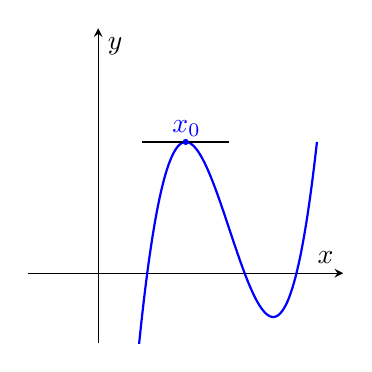
\begin{tikzpicture}
                \begin{axis}[
                xlabel=$x$,
                ylabel=$y$,
                axis equal,
                axis lines=middle,
                enlargelimits,
                xmax=5,
                xmin=-1,
                ymax=5,
                ymin=-1,
                xtick={0},
                ytick={0},
                scale only axis, 
                height=4cm, 
                width=4cm
                ]
            \addplot [blue, no marks, thick, domain=0:5, samples=1000] {(x-3)^3-3*x+10};
            \node at (2.02, 3.3) {\textcolor{blue}{$x_0$}};
            \addplot [thin] coordinates {(1, 3) (3,3)};
            \fill [blue] (2, 3) circle (0.07);
            \end{axis}
            \end{tikzpicture}
        \end{center}
        presenta in $ x_0 $ un punto di massimo locale; $ f $ è derivabile in $ x_0 $, e in questo punto la tangente è orizzontale.
        \item Per la funzione 
        \begin{center}
            \begin{tikzpicture}
                \begin{axis}[
                xlabel=$x$,
                ylabel=$y$,
                axis equal,
                axis lines=middle,
                enlargelimits,
                xmax=5,
                xmin=-1,
                ymax=5,
                ymin=-1,
                xtick={0},
                ytick={0},
                scale only axis, 
                height=4cm, 
                width=4cm
                ]
            \addplot [blue, no marks, thick, domain=0:5, samples=1000] {-sqrt(abs(x-1))+2};
            \node at (1.02, 2.3) {\textcolor{blue}{$x_0$}};
            \addplot [thin] coordinates {(0, 2) (2,2)};
            \fill [blue] (1, 2) circle (0.07);
            \end{axis}
            \end{tikzpicture}
        \end{center}
        $ x_0 $ è punto di massimo locale, ma la tangente in $ x_0 $ non è orizzontale perché non esiste.
    \end{enumerate}
}

\teorema[(di Fermat)]{difermatalleluia}{Se
    \begin{enumerate}
        \item $ f:I\to \R $, $ I $ intervallo;
        \item $ x_0 \in \mathring{I} $;
        \item $ x_0 $ punto di massimo o minimo locale;
        \item $ f $ derivabile in $ x_0 $;
    \end{enumerate}
    allora $ f'(x_0)=0 $, ovvero $ f $ ammette in $ x_0 $ tangente orizzontale.
}
\definizione{}{
    $ x_0 $ tale che $ f$ è derivabile in $ x_0 $ e $ f'(x_0)=0$ è detto \textit{punto critico} o \textit{stazionario} per $ f $.
}
\dimostrazione{difermatalleluia}{
    Studiamo il caso in cui $ x_0 $ punto di \textit{massimo} locale: \begin{equation}
        \exists\, U(x_0)\,\tc\quad \forall\,x \in U(x_0)\quad f(x)\le f(x_0)\: \bigl(\iff\, f(x)-f(x_0)\le 0\bigr)\label{eccociqui}
    \end{equation}
    Calcoliamo il limite: $\displaystyle
        \lim_{x\to x_0} \frac{f(x)-f(x_0)}{x-x_0}$: ci sono due casi.
    \begin{itemize}
        \item [(+)] Se $ x>x_0 $ \[
            \lim_{x\to x_0} \frac{f(x)-f(x_0)}{x-x_0} \underset{\footnotemark}{=}f'(x_0)\footnotetext{poiché $ f $ è derivabile in $ x_0 $}
        \]
        Vale inoltre $ f'(x_0)\le 0 $, per il teorema di permanenza del segno: infatti, nota \eqref{eccociqui}, si ha $ x-x_0>0 $.
        \item [(-)] Se $ x<x_0 $ \[
            \lim_{x\to x_0} \frac{f(x)-f(x_0)}{x-x_0} =f'(x_0)
        \]
        Inoltre $ f'(x_0)\ge 0 $ per il teorema di permanenza del segno: infatti, nota \eqref{eccociqui}, si ha $ x-x_0<0 $.
    \end{itemize}
    Allora deve essere \[
        f'(x_0)\le 0\:\land\: f'(x_0)\ge 0 \,\implies\, f'(x_0)=0
    \] %DOMANDA non mi piace questa dimostrazione, usare anche quella della piovano
}

\attenzione{
    Non vale il viceversa: un punto stazionario non implica un massimo (o un minimo).
}
\esempio{}{
    Sia $ f(x)=x^{3} $, $ \dom f=\R $: $ \forall\, x $, $ x \in \mathring{\R}$

    $ f'(x)=3x^{2} $, e $ f'(x)=0 $ $ \iff $ $ x=0 $, ma $ x_0=0 $ non è punto di massimo o minimo locale per $ f $. 

    $ x_0=0 $ è un flesso a tangente orizzontale\footnote{\hyperref[flesso]{definizione successiva}}.
}

\attenzione{Se $ x_0 $ è stazionario per $ f $, non è detto che sia massimo, minimo, o flesso a tangente orizzontale.}
\esempio{}{\label{esempiosinxquadrp}
    Data $ f(x)=\begin{cases}
        x^{2}\,\sin \frac{1}{x} & x\neq 0\\
        0 & x=0
    \end{cases} $ abbiamo verificato che $ f $ è derivabile in $ x_0=0 $, e $ f'(0)=0 $. $ x_0=0 $ è stazionario per $ f $, ma $ x_0=0 $ non è massimo, minimo o flesso. 
}
\begin{figure}
    \centering
        \begin{tikzpicture}
            \begin{axis}[
                xlabel=$x$,
                ylabel=$y$,
                axis equal,
                axis lines=middle,
                enlargelimits,
                xmax=0.05,
                xmin=-0.05,
                ymax=0.1,
                ymin=-0.1,
                xtick={0},
                ytick={0},
                scale only axis, 
                height=6cm, 
                width=6cm
                ]
            \addplot [blue, no marks, thick] file {xsin1x.csv};
            \end{axis}
        \end{tikzpicture}
    \caption{\hyperref[esempiosinxquadrp]{Esempio (\thesection.\theesempi)}}
    \label{figes:33}
\end{figure}

%TODO mancano tutte le cose successive, non si capiva assolutamente niente
% appunti di Simone Pacini
\subsection{Forme quadratiche reali ($ \K=\R$)}
Sia\marginnote{7 dic 2021} $ V $ spazio vettoriale su $ \R $, e $ \xi \in B_{S}(V, \R)  $. $ \xi $ si dice\begin{enumerate}
    \item \textit{definita positiva} se $ \xi(v,v)>0 $ $ \forall\, v \in V, v\neq \underline{0} $;
    \item \textit{definita negativa} se $ \xi(v,v)<0 $ $ \forall\, v \in V, v\neq \underline{0} $;
    \item \textit{semidefinita positiva} se $ \xi(v,v)\ge 0 $ $ \forall\, v \in V $;
    \item \textit{semidefinita negativa} se $ \xi(v,v)\le 0 $ $ \forall\, v \in V $;
    \item \textit{indefinita} se non rientra nei casi precedenti.
\end{enumerate}
\esempi{}{
    \begin{enumerate}
        \item Se $ \xi $ è un prodotto scalare, $ \xi $ è definita positiva, e $ -\xi  $ è definita negativa;
        \item considero $ \xi \in B_{S}(\R^{3}, \R)  $, tale che $ Q_{\xi}(x)=x_1^{2}+x_2^{2} $, semidefinita positiva, non definita positiva;
        \item considero $ \xi \in B_{S}(\R^{3}, \R)  $, tale che $ Q_{\xi}(x)=-x_1^{2}-x_2^{2} $, semidefinita negativa, non definita negativa;
        \item considero $ \xi \in B_{S}(\R^{3}, \R)  $, tale che $ Q_{\xi}(x)=x_1^{2}-x_2^{2} $, indefinita.
    \end{enumerate}
}

\osservazione{
    Se $ \xi  $ è definita (positiva o negativa), allora $ \xi $ è non degenere. Infatti $ \xi(v,v)\neq 0 $ se $ v\neq \underline{0} $, quindi $ \ker\xi=\{\underline{0}\} $. 
    
    Ma esistono forme bilineari indefinite non degeneri, come $ \xi \in B_{S}(\R^{3}, \R )  $, $ Q_{\xi}(x)=x_1^{2}+x_2^{2}-x_3^{2}  $
}

\teorema{eleferelicuresaij}{
    Sia $ \xi \in B_{S}(V, \R)  $, semidefinita positiva. Allora vale la disuguaglianza (di Cauchy-Schwartz) \begin{equation}
        |\xi(v,w)|^{2}\le Q_{\xi}(v) \cdot Q_{\xi}(w)\qquad \forall\, v, w \in V  
    \end{equation}
}
\dimostrazione{eleferelicuresaij}{
    \begin{itemize}
        \item Se $ Q_{\xi}(v)=0 $ $ \forall\, v \in V $ 
    
    $\implies$ $ \xi(v, w)=0 $ $ \forall\, v, w \in V $, vale il teorema.
    \item Se $ Q_{\xi}  $ non è identicamente nulla: si considerano tre casi\begin{enumerate}
        \item $ Q_{\xi}(v)\neq 0  $, $ Q_{\xi}(w)=0  $;
        \item $ Q_{\xi}(v)= 0  $, $ Q_{\xi}(w)\neq 0  $;
        \item $ Q_{\xi}(v)\neq 0 \neq Q_{\xi}(w) $;
    \end{enumerate}

    \textit{Caso 1.} $ \forall\, \lambda \in \R $, $ Q_{\xi}(v+ \lambda w)\ge 0 $ poiché $ \xi $ semidefinita positiva \[
        Q_{\xi}(v+\lambda\, w)=\xi(v+\lambda\, w, v+\lambda\, w) =\xi (v,v)+2 \lambda\xi(v, w)\ge 0
    \]
    Quindi $ Q_{\xi}(v)+2 \lambda \xi(v,w)  $ $ \forall\, \lambda \in \R $ 
    
    $\implies$ $ \xi(v,w)=0 $ e vale l'uguaglianza.

    Il \textit{caso 2.} si ricava dal caso 1. invertendo $ v $ e $ w $.

    \textit{Caso 3.} $ Q_{\xi}(v)\neq 0 \neq Q_{\xi}(w) $. So che $ \forall\, \lambda \in \R $, $ Q_{\xi}(v+\lambda\,w)\ge 0  $ \begin{multline*}
        0\le Q_{\xi}(v+\lambda\,w)=\xi(v+\lambda\,w, v+\lambda\,w)=\\=Q_{\xi}(v)+\lambda^{2}Q_{\xi}(w)+2 \lambda \xi(v,w)   
    \end{multline*} Sia \[
        p:= \lambda^{2} Q_{\xi}(w)+ 2 \lambda \xi (v,w) + Q_{\xi}(v)  
    \] $ p $ polinomio di secondo grado in $ \R_{2}[\lambda]  $.
    Poiché $ p\ge 0 $, il $ \Delta\le 0 $ 
    
$\implies$ $ \xi(v,w)^{2}- Q_{\xi}(v) \cdot Q_{\xi}(w)\le 0  $ 

$\implies$ $ |\xi(v,w)| \le Q_{\xi}(v) \cdot Q_{\xi}(w)   $\qed
    \end{itemize}
}

\proposizione{elefanterosacandido}{
    Nelle ipotesi del teorema precedente vale la disuguaglianza triangolare:\begin{equation}
        \sqrt{Q_{\xi}(v+w)}\le \sqrt{Q_{\xi}(v) }+\sqrt{Q_{\xi}(w) }\quad \forall\, v, w \in V
    \end{equation}
}
\dimostrazioneprop{elefanterosacandido}{
    Usiamo $ Q_{\xi}(v+w)=Q_{\xi}(v)+Q_{\xi}(w)+2\xi(v,w)$.
    \begin{align*}
        \left|Q_{\xi}(v+w) \right|&\le \left|Q_{\xi}(v)\right|+\left|Q_{\xi}(w) \right|+2\,\left|\xi(v,w)\right|\\
        &\le \left|Q_{\xi}(v)\right|+\left|Q_{\xi}(w) \right|+2\,\sqrt{Q_{\xi}(v) }\,\sqrt{Q_{\xi}(w) }\\
        &= \left(\sqrt{Q_{\xi}(v) }+\sqrt{Q_{\xi}(w)}\right)^{2}
    \end{align*} segue la tesi.\qed
}

\rule{7em}{.4pt}

Dato $ V $ spazio vettoriale su $ \R$, finitamente generato, e $ \xi \in B_{S}(V, \R)  $. Fisso $ \mathscr{B}=\{v_1, \cdots,v_{n}\} $ base di $ V $. Il teorema di Lagrange afferma che $ \exists\, \mathscr{B}' $ base di $ V $ ortogonale rispetto a $ \xi $, cioè tale che $ M^{ \mathscr{B}'}(\xi) $ diagonale, e quindi se $ (v)_{ \mathscr{B}'}=(x_1, \cdots, x_{n} ) $, vale $ Q_{\xi}(v)=x_1^{2}a_{11}+\cdots+ x_{n}^{2}a_{nn}    $.

Si può utilizzare il \textit{teorema spettrale}. $ \mathscr{B} $ da origine a $ M^{ \mathscr{B}}(\xi) $, se $ \mathscr{B}' $ è un'altra base $\implies$ $ M^{ \mathscr{B}'}(\xi)=\null^{t}\!P\,M^{ \mathscr{B}}(\xi)\, P $ con $ P \in \gl(n, \R) $ matrice del cambiamento di base. 

Qui si può utilizzare il teorema spettrale, $ M^{ \mathscr{B}}(\xi) $ è diagonalizzabile, ed esiste $ P \in O(n) $ tale che \[P^{-1}\, M^{ \mathscr{B}}(\xi)\,P=\begin{pmatrix}
    \lambda_1 & & \\
    & \ddots &\\
    & & \lambda_{n} 
\end{pmatrix}\] dove $ \lambda_1, \cdots, \lambda_{n}  $ sono gli autovalori di $ M^{ \mathscr{B}}(\xi) $. 

Poiché $ P \in O(n) $, $ \null^{t}\!P=P^{-1} $ 

$\implies$ $ \null^{t}\!P\,M^{ \mathscr{B}}(\xi) P = \biggl(\begin{smallmatrix}
    \lambda_1 & & \\
    & \ddots &\\
    & & \lambda_{n} 
\end{smallmatrix}\biggr) $, quindi si trova sempre una forma canonica di $ Q_{\xi}  $ in cui i coefficenti sono gli autovalori di $ M^{ \mathscr{B}}(\xi) $.

\todo{Manca un esercizio (chiesto a Simone Pacini)}

\osservazione{
    Sia $ \xi \in B_S(V, \R) $, esiste una base ortogonale di $ \xi $, $\mathscr{B}=\{v_1, \cdots, v_{n}\}$, $ \xi(v_i, v_j)=0$ $\forall\, i\neq j $ \[
        \xi(v_{i}, v_{i}  )\begin{cases}
            >0\\
            =0\\
            <0
        \end{cases}
    \] sia $ a_i:=\xi(v_i, v_i) $; si definisce $\mathscr{B}=\{v_1',\cdots, v_{n}'\}  $ dove 
    \begin{align*}
        v_i'&=v_i&\text{se }a_i=0\\
        v_i'&=\frac{v_i}{\sqrt{a_i}} &\text{se } a_i>0\\
        v_i'&=\frac{v_i}{\sqrt{-a_i}} &\text{se }a_i<0
    \end{align*}
        Risulta \[
        \xi(v_{i}', v_{i}'  )=\begin{cases}
            1 &\text{se }\xi(v_{i}, v_{i}  )>0\\
            0 &\text{se }\xi(v_{i}, v_{i}  )=0\\
            -1 &\text{se }\xi(v_{i}, v_{i}  )<0
        \end{cases}
        \]
        Si trova una base $\mathscr{B}'=\{v_1', \cdots, v_{n}'\}  $ ortogonale tale che $ \xi(v_i', v_i') \in \{-1, 0, 1\} $. Rispetto a questa base, $ Q_\xi $: \[
            Q_{\xi}(x)=x_1^{2}+ \cdots + x_{r}^{2}- x_{r+1}^{2}-\cdots-x_{r+s}^{2}\qquad r+s\le n = \dim V    
        \]

        In questo caso si dice che $ Q_{\xi} $ è in \textit{forma normale}.
} 

\esempio{}{
    Nell'esempio precedente la forma normale di $ Q_{\xi}(x)=-x_1^{2}+x_2^{2}+x_3^{2}  $
}

\teorema[(di Sylvester)]{silversdffsdf}{
    Sia $ V $ uno spazio vettoriale su $ \R $, finitamente generato. Sia $ \xi \in B_{S}(V, \R) $.
    
    Allora tutte le forme canoniche associate a $ Q_{\xi}  $ hanno lo stesso numero di coefficienti positivi ($p$) e lo stesso numero di coefficienti negativi ($q$).

    $ p+q=\rank (\xi) $ e la coppia $ (p,q) $ si dice la segnatura di $ \xi $.
}
\dimostrazione{silversdffsdf}{
    Sia $ \mathscr{C}=\{v_1, \cdots, v_{n}\}  $ una base ortogonale di $ V $ rispetto a $ \xi $, tale che $ Q_{\xi}  $ si scriva in forma normale, \[
        Q_{\xi}(v)= y_1^{2}+\cdots+ y_{p}^{2}- y_{p+1}^{2}- \cdots- y_{r}^{2}    
    \] dove $ (v)_{ \mathscr{C}}=(y_1, \cdots, y_{n} ) $, $ r=\rank \xi $.

    Quindi $ \xi(v_{i}, v_{i}  )=1 $ per $ i=1, \cdots, p $, $ \xi(v_{j}, v_{j})=-1 $ se $ j=p+1, \cdots, r $, $ \xi(v_{k}, v_{k}  )=0 $ se $ k=r+1, \cdots, n $.

    Sia $ \mathscr{C}'=\{v_1', \cdots, v_{n}'\}  $ un'altra base di $ V $ rispetto a cui $ Q_{\xi}  $ si scrive in forma normale \[
        Q_{\xi}(w) =z_1^{2}+\cdots+z_{t}^{2}-z_{t+1}^{2}-\cdots-z_{r}^{2}   
    \] dove $ (v)_{ \mathscr{C}'}=(z_1, \cdots, z_{n} ) $.

    Devo dimostrare che $ t=p $. Supponiamo per assurdo $ t<p $. Si considerino \[
        W_1= \mathscr{L}(v_1, \cdots, v_{p} )\qquad W_2= \mathscr{L}(v_{t+1}', \cdots, v_{n}'  )
    \] Vale che $ \dim W_1=p $, $ \dim W_{2}=n-t  $, \[\dim W_1+\dim W_2 = p+n-t>0\] 
    
    $\implies$ $ W_1\cap W_2 \neq \{\underline{0}\}$ 
    
    $\implies$ $ \exists v \in W_1\cap W_2 $, $ v\neq 0 $.
    
    Si ha quindi $ Q_{\xi}(v)>0  $ poiché $ \restriction{\xi}{W_1\times W_1}$ è definita positiva, ma inoltre $ Q_{\xi}(v)\le 0  $, poiché $ \restriction{\xi}{W_2\times W_2} $ è semidefinita negativa. Assurdo.
    
    $\implies$ $ t\ge p $. 
    
    In modo analogo si dimostra che $ t>p $ porta ad un assurdo (esercizio%ESERCIZIO fare per esercizio
    ) 
    
    $\implies$ $ t=p $\qed
}

Si definisce \textit{segnatura} di una $ \xi \in B_{S}(V, \R)$ la coppia di numeri $ (p,q) $, con $p $ il numero di coefficienti positivi di una forma canonica di $ \xi $ e $ q $ il numero di coefficienti negativi di una forma canonica di $ \xi $.

Per calcolare la forma canonica si fissa $ \mathscr{B} $ base di $ V $ e si trovano gli autovalori di $ M^{ \mathscr{B}}(\xi) \in \R^{n,n}$ simmetrica.

\definizione{}{
    Sia $ A \in \R^{n,n} $ una matrice simmetrica. Si definisce la \textit{segnatura} di $ A $ come la coppia di numeri $ (p,q) $, dove $ p $ è il numero di autovalori positivi di $ A $, mentre $ q $ è il numero degli autovalori negativi si $ A $, entrambi contati con la loro molteplicità.
}

\corollario{lklkmlkmlsdfjoijoijoijsdf}{
    Siano $ A, B \in \R^{n,n}$ due matrici simmetriche. Se $ A $ e $ B $ sono congruenti $\implies$ $ A $ e $ B $ hanno la stessa segnatura.
}{}

Il viceversa non è vero, controesempio: $ A=\bigl(\begin{smallmatrix}
    1 & 0 \\ 0 & 2
\end{smallmatrix}\bigr) $, $ B=\bigl(\begin{smallmatrix}
    1 & 0 \\ 0 & 1
\end{smallmatrix}\bigr) $ hanno la stessa segnatura $ (2, 0)$ ma non sono congruenti poiché $ \det A \neq \det B $

\rule{7em}{.4pt}

Data $ \xi \in B_{S}(V, \R)$ voglio trovare la forma normale di $ Q_{\xi}  $ ``a occhio'' (senza dover implementare il calcolo degli autovalori).

Fisso $ \mathscr{B} $ base di $ V $, considero $ M^{ \mathscr{B}}(\xi)=A $ e $ r(\lambda)=\det (A-\lambda\id) $.

La segnatura di $ \xi $ è $ (p, q) $, dove $ p $ è il numero di radici positive di $ r(\lambda) $, mentre $ q $ è il numero di radici negative di $ r(\lambda) $.

\paragraph{Regola di Cartesio} Sia $ r \in \R[x] $ un polinomio di grado $ n $, \[
        r(x)=a_0+a_1\,x+\cdots+a_{n}\, x^{2} 
    \] 
    
    $\implies$ il numero di radici positive di $ r(x) $ è il numero di variazione di segno dei coefficienti $ a_0, a_1, \cdots, a_{n}$, consecutivi tralasciando i coefficienti nulli.

\esempio{
    Sia $ \xi \in B_{S}(\R^{3}, \R)  $ definita da $ Q_{\xi}(x)=2x_1^{2}+4x_1x_3+x_2^{2}-x_3^{2}   $. Calcolo la forma normale di $ Q_{\xi}$.
    \[
        M^{ \mathscr{B}}(\xi)=\begin{pmatrix}
            2 & 0 & 2\\
            0 & 1 & 0\\
            2 & 0 & -1
        \end{pmatrix}\qquad p(\lambda)=-\lambda^{3}+2 \lambda^{2}+5 \lambda-6
    \]

    Si deduce che $ p $ ha due radici positive. $ p(0)=-6\neq 0 $, quindi $ p $ non ha radici nulle, allora $ p $ ha una radice negativa.

    La forma normale di $ Q_{\xi}  $ è \[
        Q_{\xi}(y)=y_1^{2}+y_2^{2}-y_3^{2}
    \]
}
\end{document}